\documentclass[12pt,openany]{book}

\usepackage[utf8]{inputenc}
\usepackage[T1]{fontenc}
\usepackage{microtype}
\usepackage{amsmath,amssymb}
\usepackage{geometry}
\usepackage[colorlinks=true, linkcolor=black, citecolor=black, urlcolor=blue]{hyperref}
\usepackage{setspace}
\usepackage{tikz}
\usetikzlibrary{shapes,positioning,calc,decorations.pathreplacing}
\usepackage{titlesec}
\usepackage{fancyhdr}
\usepackage[most]{tcolorbox}
\usepackage{graphicx}

\geometry{inner=1.2in, outer=1in, top=1in, bottom=1in}
\onehalfspacing
\emergencystretch=1em

% --- Custom chapter heading style ---
\titleformat{\chapter}[display]
  {\normalfont\huge\bfseries}
  {\titlerule[1pt]\vspace{4pt}\Large\chaptertitlename\ \thechapter}
  {0pt}
  {\titlerule[1pt]\vspace{8pt}\Huge}
\titlespacing*{\chapter}{0pt}{-20pt}{30pt}

% --- Running headers/footers ---
\pagestyle{fancy}
\setlength{\headheight}{27.11469pt}
\addtolength{\topmargin}{-15.11469pt}
\fancyhf{}
\fancyhead[LE]{\slshape\leftmark}
\fancyhead[RO]{\slshape\rightmark}
\fancyfoot[C]{\thepage}

\renewcommand{\headrulewidth}{0.4pt}
\fancypagestyle{plain}{%
  \fancyhf{}%
  \fancyfoot[C]{\thepage}% 
  \renewcommand{\headrulewidth}{0pt}%
}

% --- Boxed environments ---
\newtcolorbox{definition}[1][]{%
  colback=blue!5, colframe=blue!60!black,
  fonttitle=\bfseries, title={#1},
  breakable, enhanced,
  before upper={\parindent15pt},
  boxrule=1pt, arc=3pt
}

\newtcolorbox{keyinsight}[1][]{%
  colback=green!5, colframe=green!50!black,
  fonttitle=\bfseries, title={#1},
  breakable, enhanced,
  before upper={\parindent15pt},
  boxrule=1pt, arc=3pt
}

\newtcolorbox{historicalsource}[1][]{%
  colback=orange!5, colframe=orange!70!black,
  fonttitle=\bfseries, title={#1},
  breakable, enhanced,
  before upper={\parindent15pt},
  boxrule=1pt, arc=3pt
}

\title{The Mathematics of Oppression:\\A Set-Theoretic Framework for Analyzing Systems of Domination}
\author{Emmanuel Theodore}
\date{}

\begin{document}

% --- Half-title page ---
\thispagestyle{empty}
\vspace*{\fill}
\begin{center}
{\Huge\bfseries The Mathematics of Oppression}
\end{center}
\vspace*{\fill}
\cleardoublepage

% --- Full title page ---
\maketitle

% --- Front matter ---
\frontmatter
\tableofcontents
\listoffigures

\chapter*{Preface}
\addcontentsline{toc}{chapter}{Preface}

This book develops a formal mathematical framework for analyzing systems of oppression using set theory, discrete mathematics, and historical analysis. The framework identifies four architectural components common to all oppressive systems: (1) asymmetric autonomy restriction between In-groups and Out-groups, (2) selective empathy that validates In-group suffering while dismissing Out-group harm, (3) ideological justification through spurious claims, and (4) resistance to structural critique.

Rather than presenting the full mathematical architecture in the abstract, this book introduces each formal variable at the exact historical moment the Elite were forced to invent it. The reader watches the system being built, tier by tier, as the Elite iteratively patched their security vulnerabilities: the Out-group ($O_{\text{racialized}}$) created in 15th-century Portugal; the Buffer Class ($I_{\text{buffer}}$) invented after Bacon's Rebellion; the Puppet Class ($P_{\text{uppet}}$) prototyped at the Constitutional Convention and scaled through Gilded Age Tweedism; and the Enforcement Class ($F_{\text{enforce}}$) evolved from slave patrols to modern policing. Only after all five tiers have been historically constructed does the complete 5-Tier Set-Theoretic Hierarchy---governed by the Predatory Min-Max Function---appear in full.

Through this iterative analysis of American racism---tracing the algorithm of Elite extraction from Portuguese racialization through the invention of whiteness, the 13th Amendment loophole, redlining, the War on Drugs, and the present-day cannibalization of the In-group---I demonstrate that the Out-group targeted by systemic oppression \textit{expands} over time, progressively encompassing groups once part of the In-group. This expansion reveals that oppressive systems serve not the nominal In-group but an Elite class ($E \subset I$) that uses division to prevent solidarity. The architecture of this system operates through recognizable, formalizable patterns that can be identified and resisted.

% --- Main matter ---
\mainmatter
\chapter{Redefining Racism}

This paper proposes a mathematical framework for understanding systems of oppression---social arrangements that systematically disadvantage a racialized Out-group ($O_{\text{racialized}}$) while advantaging an In-group ($I$), though the true beneficiaries are a small Elite class ($E \subset I$) that architects the system. The framework reveals a five-tier operational hierarchy: the Elite ($E$) extracts value, the Puppet Class ($P_{\text{uppet}}$) writes the laws, the Enforcement Class ($F_{\text{enforce}}$) physically actuates the extraction, the Buffer Class ($I_{\text{buffer}}$) receives psychological wages in lieu of material benefit, and $O_{\text{racialized}}$ bears the compounding burden of policy after policy. Traditional analyses of oppression often focus on individual prejudice or specific policy outcomes. However, such approaches fail to capture the \textit{structural} dimensions of oppression: the recurring patterns, the self-reinforcing mechanisms, and the remarkable consistency of design across different systems and scales.

The central thesis of this paper is that systems of oppression share a common \textbf{architecture of control}---a formal structure that can be identified mathematically regardless of the specific groups involved or the historical context. This architecture consists of:
\begin{enumerate}
    \item \textbf{Asymmetric autonomy restriction}: Policies and norms that constrain the Out-group's freedom while preserving the In-group's
    \item \textbf{Selective empathy}: Validation of In-group suffering while dismissing or pathologizing Out-group harm
    \item \textbf{Ideological justification}: Narratives that naturalize the asymmetry through spurious claims
    \item \textbf{Resistance to structural critique}: Mechanisms that deflect analysis from the system to individual behavior
\end{enumerate}

To develop and validate this framework, I examine \textbf{racism} as the primary case study---specifically, the American system of racial oppression from its colonial origins to the present. Racism provides an ideal test case because of its extensive historical documentation, its clear policy mechanisms, and its ongoing relevance. Through set-theoretic analysis, I demonstrate that racism exhibits all four architectural components and, crucially, that $O_{\text{racialized}}$ has \textit{expanded} over time rather than contracted.

This expansion reveals a deeper truth: the system does not ultimately serve the racial In-group but rather the Elite class ($E \subset I$) that uses racial division to prevent cross-group solidarity. The ``wages of whiteness'' \cite{roediger, dubois}---psychological compensation offered to the buffer class $I \setminus E$---substitute for material advancement while $E$ extracts value from both groups.

The architecture of this system---which I formalize as a Predatory Min-Max Function optimizing Elite extraction against class resistance---operates through recognizable patterns that can be formalized, identified, and resisted across contexts.

\textbf{A critical methodological note}: Comparing the \textit{architecture} of different oppressive systems does not equate their \textit{phenomenology}. This paper analyzes design principles---how asymmetry is created, justified, and maintained---not magnitudes of suffering. Recognizing shared structure illuminates how systems of domination reproduce themselves; it does not diminish the unique gravity of any particular manifestation.

\section{Racism as Primary Example}

\textbf{The Problem with Traditional Definitions}

Traditional definitions of racism reveal a troubling pattern: they relegate the systemic dimension to secondary or tertiary status, often buried as the third or fourth definition in dictionaries---the ``cliff notes'' version that few people encounter or use. Consider typical definitional hierarchies:

\begin{enumerate}
    \item \textbf{Primary definition}: Individual prejudice or discrimination based on race
    \item \textbf{Secondary definition}: Belief in racial superiority
    \item \textbf{Tertiary definition} (if present at all): Systemic or institutional discrimination
\end{enumerate}

This ordering is not merely unfortunate---it is \textbf{fundamentally backwards}. By centering individual prejudice, these definitions obscure the cardinal reality: \textit{the systemic element is the primary operation}. The interpersonal manifestations---individual prejudice, discriminatory actions, racial animus---are \textit{downstream products} created to maintain the systemic structure, not the cause of it.

\textbf{Reversing the Causal Arrow}

The conventional framing suggests this causal relationship:
\[
\text{Individual Prejudice} \rightarrow \text{Discriminatory Actions} \rightarrow \text{Systemic Outcomes}
\]

This implies that if we eliminate individual prejudice, systemic racism will disappear. But history reveals the opposite causal structure:
\[
\text{Elite Economic Interests} \rightarrow \text{Systemic Racialization} \rightarrow \text{Interpersonal Prejudice}
\]

As demonstrated in Chapter 2, interpersonal racism---the attitudes, beliefs, and prejudices held by individuals---\textit{was deliberately created to justify and maintain the systemic structure}. Zurara's racialization of Africans as subhuman was not a spontaneous expression of Portuguese prejudice; it was commissioned work designed to justify a system of unlimited exploitation \cite{zurara, biewen}. The interpersonal followed the systemic, not vice versa (see Figure~\ref{fig:causal_reversal}).

\begin{figure}[htbp]
\centering
\begin{tikzpicture}[
    box/.style={draw, thick, rounded corners=3pt, minimum height=0.9cm, minimum width=2.6cm, align=center, font=\small},
    arr/.style={->, thick, >=stealth},
    scale=0.95
]
    % --- Conventional (incorrect) row ---
    \node[font=\small\bfseries, red!60] at (-5.8,1.5) {Conventional};
    \node[font=\small\bfseries, red!60] at (-5.8,1.0) {(incorrect)};
    \node[box, fill=red!10, draw=red!40] (a1) at (-2.5,1.25) {Individual\\Prejudice};
    \node[box, fill=red!10, draw=red!40] (a2) at (2,1.25) {Discriminatory\\Actions};
    \node[box, fill=red!10, draw=red!40] (a3) at (6.5,1.25) {Systemic\\Outcomes};
    \draw[arr, red!40] (a1) -- (a2);
    \draw[arr, red!40] (a2) -- (a3);
    % Strike-through
    \draw[very thick, red!50] (-4.5,1.25) -- (8.5,1.25);

    % --- Reversal arrow ---
    \draw[arr, very thick, black!70, double] (1.5,0.3) -- (1.5,-0.5);
    \node[font=\footnotesize\bfseries, black!70] at (3.2,-0.1) {Causal reversal};

    % --- Correct row ---
    \node[font=\small\bfseries, green!50!black] at (-5.8,-1.25) {Actual};
    \node[font=\small\bfseries, green!50!black] at (-5.8,-1.75) {(historical)};
    \node[box, fill=green!15, draw=green!50!black] (b1) at (-2.5,-1.5) {Elite Economic\\Interests};
    \node[box, fill=green!15, draw=green!50!black] (b2) at (2,-1.5) {Systemic\\Racialization};
    \node[box, fill=green!15, draw=green!50!black] (b3) at (6.5,-1.5) {Interpersonal\\Prejudice};
    \draw[arr, green!50!black, very thick] (b1) -- (b2);
    \draw[arr, green!50!black, very thick] (b2) -- (b3);
\end{tikzpicture}
\caption{\textbf{The Causal Reversal.} The conventional framing (top, struck through) assumes individual prejudice produces systemic outcomes. The historical evidence (bottom) reveals the opposite: Elite economic interests created systemic racialization, which then cultivated interpersonal prejudice to maintain the structure.}
\label{fig:causal_reversal}
\end{figure}

\textbf{The Linguistic Evidence}

Moreover, traditional definitions overlook a fundamental linguistic aspect: the suffix ``-ism'' in ``racism'' already denotes a \textit{system}. We recognize this in other contexts:
\begin{itemize}
    \item \textbf{Capitalism}: A \textit{system} of economic organization, not just individual acts of trade
    \item \textbf{Feudalism}: A \textit{system} of social hierarchy, not just individual lord-serf relationships
    \item \textbf{Colonialism}: A \textit{system} of territorial exploitation, not just individual acts of conquest
\end{itemize}

Yet with racism, we persistently treat it as a collection of individual attitudes rather than recognizing the systemic nature embedded in the very structure of the word. This is not accidental---it serves to deflect attention from the structural mechanisms that create and perpetuate racial inequality.

\textbf{The Critical Distinction: Racism is Not Prejudice}

This analysis reveals a fundamental conceptual error in conflating racism with prejudice or bias. The distinction is not one of degree but of \textit{kind}:

\begin{quote}
\textbf{Prejudice or bias}: Individual attitudes, stereotypes, or discriminatory behaviors based on group membership. These are interpersonal phenomena that can exist in any direction and between any groups.

\textbf{Racism}: A \textit{system of oppression} that weaponizes prejudice and bias into structural mechanisms of exploitation and control. Racism takes individual prejudice and transforms it through institutionalization into a self-perpetuating apparatus that serves Elite economic interests.
\end{quote}

\textbf{Without the systemic element, there is no racism---there is only prejudice.} The system is not an optional feature or a more severe manifestation; it is the \textit{defining characteristic} that distinguishes racism from generic bias. Consider:

\begin{itemize}
    \item A person holding negative stereotypes about another group = \textbf{prejudice}
    \item A system that codifies those stereotypes into law, policy, and institutional practice to extract labor and prevent solidarity = \textbf{racism}
\end{itemize}

Racism is the process of taking interpersonal prejudice and bias---which exist across all human societies---and \textbf{weaponizing them} into a system that:
\begin{enumerate}
    \item \textbf{Institutionalizes} prejudice through policy ($P$)
    \item \textbf{Concentrates} harm at the intersection $O_{\text{racialized}} \cap P$
    \item \textbf{Naturalizes} the resulting disparities through ideology
    \item \textbf{Compounds} disadvantage over time through the mechanisms described in Chapter~4
    \item \textbf{Serves} Elite economic interests by preventing working-class solidarity
\end{enumerate}

This distinction has profound implications. An individual can hold prejudices without participating in racism if those prejudices are not institutionalized into systems of power. Conversely, an individual can participate in and benefit from racist systems even while holding no conscious prejudice---because racism operates \textit{systemically}, through policies and structures, not merely through individual attitudes.

The conflation of racism with prejudice is not merely imprecise---it is \textbf{functionally useful to the system}. By treating them as synonymous, we:
\begin{itemize}
    \item Suggest that eliminating individual prejudice eliminates racism
    \item Enable individuals to disavow racism by disavowing prejudice
    \item Obscure the structural mechanisms that create and maintain racial hierarchy
    \item Deflect attention from the Elite class that benefits from racial division
    \item Make structural analysis seem like an overreaction to individual attitudes
\end{itemize}

The system is \textit{the point}. Racism is fundamentally and irreducibly systemic. Without the system, we're discussing prejudice, bias, or discrimination---real phenomena, but categorically different from racism as a system of oppression.

\textbf{Why the Misdirection Matters}

Centering individual prejudice as the primary definition of racism accomplishes several functions that protect the systemic structure:

\begin{enumerate}
    \item \textbf{Individualizes responsibility}: If racism is primarily individual prejudice, then solutions focus on changing hearts and minds rather than dismantling structures.
    
    \item \textbf{Obscures Elite benefits}: Individual-focused definitions hide the fact that racism serves Elite economic interests by preventing working-class solidarity.
    
    \item \textbf{Enables plausible deniability}: Individuals can claim ``I'm not racist'' (meaning ``I don't hold personal prejudice'') while participating in and benefiting from racist systems.
    
    \item \textbf{Makes structural critique seem extreme}: If racism is ``just'' individual prejudice, then analyzing systemic structures appears to be overreach or ``seeing racism everywhere.''
    
    \item \textbf{Perpetuates the system}: By misidentifying the disease (treating symptoms rather than cause), individual-focused definitions ensure the system persists.
\end{enumerate}

\textbf{The Correct Hierarchy}

A proper definition must reverse the conventional ordering, placing systemic policies at the center (see Figure~\ref{fig:hierarchy_inversion}):

\begin{enumerate}
    \item \textbf{Primary}: Racism is a \textit{system} of policies and structures that create and maintain racial hierarchies for Elite economic benefit
    \item \textbf{Secondary}: This system is justified through ideological narratives that naturalize racial categories and hierarchies
    \item \textbf{Tertiary}: These narratives manifest in interpersonal prejudices and discriminatory actions that reinforce the system
\end{enumerate}

This ordering reflects the historical reality established in Chapter 2: systemic racialization came first, ideological justification followed, and interpersonal prejudice was cultivated to maintain the structure. The interpersonal is real and harmful, but it is \textit{epiphenomenal}---a surface manifestation of the deeper systemic operation.

\begin{figure}[htbp]
\centering
\begin{tikzpicture}[
    layer/.style={draw, thick, minimum width=4.8cm, minimum height=0.85cm, align=center, font=\small},
    scale=0.95
]
    % --- Conventional (left) ---
    \node[font=\small\bfseries] at (-3.5,3.2) {Conventional Hierarchy};
    % Primary (largest, top)
    \node[layer, fill=red!25, minimum width=5.2cm] (c1) at (-3.5,2.2) {\textbf{1. Individual Prejudice}};
    \node[layer, fill=red!15, minimum width=4.2cm] (c2) at (-3.5,1.15) {\textbf{2. Belief in Superiority}};
    \node[layer, fill=red!8, minimum width=3.2cm] (c3) at (-3.5,0.1) {\textbf{3. Systemic} (if present)};
    \node[font=\scriptsize, red!60] at (-3.5,-0.5) {$\uparrow$ buried, rarely referenced};

    % --- Arrow between ---
    \draw[->, very thick, black!60, double] (0.2,1.15) -- (1.6,1.15);
    \node[font=\footnotesize\bfseries, black!60, align=center] at (0.9,0.5) {Must\\invert};

    % --- Correct (right) ---
    \node[font=\small\bfseries] at (5.3,3.2) {Correct Hierarchy};
    % Primary (largest, top)
    \node[layer, fill=green!25, minimum width=5.2cm] (r1) at (5.3,2.2) {\textbf{1. Systemic Policies}};
    \node[layer, fill=green!15, minimum width=4.2cm] (r2) at (5.3,1.15) {\textbf{2. Ideological Narratives}};
    \node[layer, fill=green!8, minimum width=3.2cm] (r3) at (5.3,0.1) {\textbf{3. Interpersonal Prejudice}};
    \node[font=\scriptsize, green!50!black] at (5.3,-0.5) {$\uparrow$ epiphenomenal, downstream};
\end{tikzpicture}
\caption{\textbf{Inverting the Definitional Hierarchy.} Conventional definitions (left) bury the systemic dimension as a tertiary afterthought. The correct hierarchy (right) places systemic policies at the top, recognizing that ideological narratives and interpersonal prejudice are downstream products of the system, not its cause.}
\label{fig:hierarchy_inversion}
\end{figure}

To address this fundamental gap in conventional definitions, I propose a new definition that places the systemic element where it belongs: at the center of analysis. This definition emphasizes racism as a system of oppression, deeply rooted in historical practices and policies that categorize individuals based on perceived racial differences---a system deliberately created by Elites to break class solidarity and maintain exploitable labor.


\chapter{Version 1.0: Initializing the Vector (15th-Century Portugal)}
\label{ch:portugal}

\begin{tcolorbox}[colback=black!5, colframe=black!70, fonttitle=\bfseries\ttfamily, title=RUNTIME LOG: 1486 (LISBON{,} PORTUGAL)]
\ttfamily\small
\textbf{System Stress} ($\min$: class resistance): HIGH --- Domestic labor shortage threatening agricultural capital. Existing moral framework constrains exploitation of Christians.\\
\textbf{Capital} ($\max$: extraction output): STAGNANT --- Sugar trade demands labor the current moral economy cannot supply.\\
\textbf{Active Patch}: Compiling Version 1.0\ldots\\
\textbf{Variables Deployed}: The Elite Class ($E$), The Out-group ($O_{\text{racialized}}$), The In-group ($I$).\\
\textbf{Executing Function}: The Implicit Contract (Issuing the Psychological Wage).\\
\textbf{Result}: Extraction Algorithm initialized. \textbf{[POLICY]} \textit{Dum Diversas} (1452) and \textit{Romanus Pontifex} (1455) authorize unlimited exploitation. \textbf{[POLICY]} \textit{Casa dos Escravos} (1486) institutionalizes state-managed extraction. Vector established.
\end{tcolorbox}

\medskip

If we are to understand the modern mathematics of oppression, we must first examine the original source code. Systemic racism was not an accident of human nature, nor was it a spontaneous cultural prejudice that slowly calcified into law. It was a calculated, mathematical technology engineered by an Elite class to solve a specific economic problem.

To find the compilation date of this algorithm, we must look to 15th-century Portugal. The Portuguese Crown---the Elite---was expanding its global empire, driven by the highly lucrative sugar trade. However, the Elite faced a critical system stressor: a severe shortage of cheap, domestic labor to work the plantations. To scale their capital, they needed an entirely new class of labor that could be extracted indefinitely, without the pesky overhead of wages, rights, or the threat of peasant revolts.

They did not just need workers; they needed to \textbf{bifurcate the human population}. They needed to simultaneously mint two new variables: the Out-group and the In-group.

\subsection{The Vector Equation of Racism}

Traditional sociological models frequently err by calculating prejudice as a \textit{scalar} quantity. In mathematics and physics, a scalar is a metric possessing magnitude but lacking a definitive direction (like temperature or speed). An individual's personal bias or anger is a scalar---emotional weight, but it lacks the institutional momentum to alter society.

Under the strict parameters of the mathematics of oppression, systemic racism cannot be a scalar. It must be defined as a \textbf{vector}. A vector possesses both magnitude \textit{and} a specific, irreversible direction.

\[
\vec{R}_{\text{acism}} = M_{\text{agnitude}} \cdot \hat{d}_{\text{state}}
\]

In this equation, $M$ represents the magnitude of human prejudice. But the true engine of the equation is $\hat{d}_{\text{state}}$---the top-down directional force provided by the state.

The Portuguese Elite engineered this vector through a dual-authorization mechanism. First, they secured the moral architecture via the Catholic Church (such as the 1452 Papal Bull \textit{Dum Diversas}) \cite{dumdiversas}. Second, they built the legal infrastructure, establishing the \textit{Casa dos Escravos} (House of Slaves) in Lisbon in 1486. By royal decree, all enslaved Africans had to be processed and taxed through this specific state customs house. The Elite provided the directional force ($\hat{d}_{\text{state}}$) that transformed baseline xenophobia into a state-managed, highly profitable extraction machine.

\section{Portuguese Class Dynamics and the Elite's Dilemma}

Before understanding the invention of race, we must first understand the class dynamics that necessitated it. In 15th century Portugal, as in much of medieval Europe, society had achieved a degree of class solidarity that constrained Elite exploitation. The feudal system, while hierarchical, operated within a shared moral framework: all humans, regardless of status, were part of the same moral community. Peasants and nobility alike were Christians, subjects of the same crown, and---critically---recognized as human beings with souls.

This moral inclusion created practical limits on exploitation. While the Elite could extract labor through serfdom and taxation, they faced constraints:
\begin{itemize}
    \item \textbf{Religious doctrine}: The Catholic Church, despite supporting hierarchy, imposed limits on the treatment of Christians. Enslavement of fellow Christians was prohibited or heavily restricted.
    \item \textbf{Legal protections}: Even serfs had some legal standing---they could not be killed arbitrarily, families could not be separated at will, and certain customary rights were recognized.
    \item \textbf{Social cohesion}: Shared identity as Portuguese, as Christians, and as humans created bonds that could translate into solidarity against Elite overreach.
    \item \textbf{Demographic limits}: The available labor pool consisted of people who belonged to the moral community, limiting how brutally they could be exploited without risking rebellion or moral condemnation.
\end{itemize}

The Portuguese Elite faced a fundamental problem: \textbf{how to create a permanent slave class without violating the moral framework that constrained exploitation of the existing population}. They needed a labor force that could be worked to death, families that could be separated, and people who could be treated as property---all without triggering the moral and legal protections that applied to humans.

The solution was elegant and horrifying: \textbf{remove an entire category of people from the moral community by declaring them non-human}.
\section{The Invention of Race as Moral Exclusion}

The concept of race and the systemic nature of racism have their roots deeply embedded in this Elite need to break class solidarity and create a slave class unconstrained by moral limits. A pivotal figure in this narrative is Gomes de Zurara, whose work in the 1450s laid the groundwork for the racialization of African peoples. Commissioned by the Portuguese monarchy, Zurara authored a chronicle that justified the enslavement of African individuals by portraying them as a monolithic group, inherently inferior and \textit{subhuman} \cite{zurara, kendi}. 

This was not merely prejudice---it was \textbf{ontological exclusion}. Zurara's narrative did not simply claim Africans were inferior humans; it positioned them as \textit{a separate species}, more akin to animals than people. This act of lumping together the diverse peoples of Africa into a single, derogatory category represented an unprecedented move towards institutionalizing race as a basis for systemic oppression.

Dr.\ Ibram X.\ Kendi highlights Zurara's role in inventing race and racism, noting that his descriptions were instrumental in justifying the Portuguese slave trade \cite{kendi}. Zurara's narrative served not only as a moral and intellectual justification for the kidnapping and enslavement of African people but also set a precedent for European engagement with sub-Saharan Africa. Portugal, thus, became the first European nation to sail directly to sub-Saharan Africa for the purpose of capturing human beings for enslavement.
\section{The Original Implicit Contract and the Psychological Wage}

Minting the Out-group solved the Elite's labor shortage, but it introduced a secondary vulnerability. The Portuguese Elite still had to manage their own impoverished, starving peasant class. If the working class realized that the Elite were hoarding all the wealth generated by this new extraction model, the system could crash via a populist revolt.

To stabilize the system, the Elite executed a psychological patch: the \textbf{Original Implicit Contract}.

You cannot mathematically define an Out-group without simultaneously creating an \textbf{In-group}. By legally defining the Out-group as subhuman commodities through the \textit{Casa dos Escravos}, the Elite automatically established the In-group ($I$)---their own peasantry---as the permanent, artificial floor of humanity.

\begin{quote}
\textit{``You may be poor, you may be exploited, but you will never be slaves. Your children will never be slaves. We do not enslave humans, and these Africans are not human---they are a subspecies, no different from cattle. Therefore, there is no reason not to exploit their labor, and your humanity is secured by their exclusion from humanity.''}
\end{quote}

Instead of distributing physical wealth or capital to the In-group, the Elite compensated them with a \textbf{Psychological Wage} ($\psi$). The mathematical function of the contract is written as:

\[
S_{\text{tatus}}(I) = \text{Base\_Humanity} + \psi
\]
\[
S_{\text{tatus}}(I) > S_{\text{tatus}}(O_{\text{racialized}})
\]

The contract dictated that no matter how destitute, hungry, or exploited the In-group peasant was, they retained the exclusive legal status of ``human.'' They could not be commodified or legally processed as property.

This was a stroke of algorithmic genius. The Elite pacified their own working class without spending a single coin, buying their loyalty entirely through the distribution of \textit{optical superiority}. The In-group accepted their economic subjugation because the system guaranteed them social supremacy over the Out-group.

\begin{definition}[Slave Capitalism]
\textbf{Slave capitalism}: a distinct economic model that combines capitalist accumulation with racialized slave labor, in which the Elite secures working-class complicity through an implicit contract that offers racial status in exchange for tolerating---and enforcing---the ontological exclusion of an enslaved population from the moral community.
\end{definition}

This contract accomplished several objectives for the Elite:

\begin{enumerate}
    \item \textbf{Broke class solidarity}: Portuguese workers could no longer identify with enslaved Africans as fellow laborers because Africans were defined as non-human. Any solidarity based on shared exploitation was severed by the ontological divide.
    
    \item \textbf{Created psychological compensation}: Poor Portuguese gained status not through material improvement but through racial categorization. The ``wages of whiteness'' (though the term would emerge later) began here: your poverty matters less when you are assured you belong to the human race and others do not.
    
    \item \textbf{Eliminated moral constraints}: By removing Africans from the moral community, the Elite eliminated the religious, legal, and social protections that constrained exploitation. Africans could be worked to death, families could be torn apart, children could be sold---none of the protections afforded to humans applied.
    
    \item \textbf{Secured labor expansion}: The Elite gained access to a theoretically unlimited labor supply that could be brutally exploited without triggering the moral frameworks that protected Portuguese workers.
    
    \item \textbf{Prevented future solidarity}: The racial framework ensured that even if African-descended peoples gained freedom, the ontological divide would persist, preventing alliances between exploited groups across racial lines.
\end{enumerate}

The model proved extraordinarily profitable for the Elite class, generating wealth accumulation at scales previously impossible under feudalism or wage labor systems \cite{williams, robinson}. Critically, the Implicit Contract and its psychological wage would be replicated wherever the algorithm was exported---across the Atlantic to the Americas, and eventually across the entire colonial world. The enforcement apparatus, the geographic displacement, and the modern continuity of this slave capitalism will be traced in their proper chronological positions as the algorithm iterates through its subsequent versions.

\section{Introducing the First Three Variables: The Elite ($E$), the Out-group ($O_{\text{racialized}}$), and the In-group ($I$)}

The historical narrative of this chapter has demonstrated the system's three foundational actors in operation: an Elite class that engineers the extraction, a racialized Out-group that bears its burden, and an In-group whose complicity is purchased through the psychological wage. We now formalize these actors mathematically---the first three variables in what will ultimately become a five-tier hierarchy, each tier introduced at the historical moment the Elite were forced to invent it.

Utilizing set theory, we define the three variables of the extraction algorithm as they emerged from the Portuguese innovation:

\begin{enumerate}
    \item \textbf{The True Elite ($E$):} The hyper-concentrated capital class (representing approximately 0.002\% of the population). They do not govern; they \textit{own}. Their primary function is dictating the core parameters of the extraction system. They are entirely insulated from the physical consequences of the system. Formally, $E \subset I$---the Elite are a subset of the In-group, but their interests are fundamentally distinct from the broader In-group they claim to represent.

    \item \textbf{The Out-group ($O_{\text{racialized}}$):} The primary extraction pool---those subjected to racialization, initially African peoples and their descendants---systematically stripped of accumulated capacity ($O_t^{\text{capacity}}$) through compounding historic and modern policies.

    \item \textbf{The In-group ($I$):} The working-class population from which the Elite originates but whose material interests the Elite actively betrays. The In-group was created simultaneously with the Out-group through the Implicit Contract: by legally defining $O_{\text{racialized}}$ as subhuman, the Elite automatically established $I$ as the permanent floor of humanity. The In-group is compensated not with material wealth but with the psychological wage ($\psi$), ensuring that $S_{\text{tatus}}(I) > S_{\text{tatus}}(O_{\text{racialized}})$ at all times. This variable will later be refined into the \textbf{Buffer Class} ($I_{\text{buffer}}$) after Bacon's Rebellion (Chapter~3), when the Elite formalize the racial partition with legal force.
\end{enumerate}

The foundational inequality of this embryonic system is therefore three-tiered:
\[
\text{Benefit}(E) \gg \text{Benefit}(I) > \text{Benefit}(O_{\text{racialized}})
\]
where $\text{Benefit}(I)$ consists primarily of $\psi$ (the psychological wage) rather than material extraction, and $\text{Benefit}(E)$ reflects the material wealth extracted from $O_{\text{racialized}}$ and, covertly, from $I$ itself.

As the historical timeline will demonstrate, this three-variable system proved insufficient. The Elite were forced to invent additional tiers---each one a patch for a specific security flaw---until the full architecture was complete. We will introduce each tier at the moment of its invention.

\textbf{A Note on Scope and Specificity}: This model is specifically designed to analyze racism as a unique system rooted in the 15th century racialization of African peoples for the purposes of enslavement and colonial exploitation. The notation $O_{\text{racialized}}$ reflects this historical specificity. While the mathematical architecture may share structural similarities with other systems of oppression, this paper focuses on racism's particular genealogy and mechanisms. The subscript ``racialized'' anchors the mathematical formalism to the historical narrative, ensuring that the model captures the unique features of racism rather than generic intergroup conflict.

\section{Institutional Legitimation: The Role of Church and Science}

The dehumanization of the African diaspora required more than political decree---it demanded \textbf{institutional legitimation} from society's most authoritative institutions. Both the Church and Science were enlisted, willingly or through institutional capture, to provide the moral and intellectual frameworks that naturalized the ontological exclusion of African peoples.

\textbf{The Church: Theological Justification for Ontological Exclusion}

The Catholic Church, despite its doctrine that all humans possess souls and are created in God's image, was systematically co-opted to support racialization:

\begin{enumerate}
    \item \textbf{The Curse of Ham doctrine}: Theologians reinterpreted the biblical story of Ham (Genesis 9:20-27) to claim that Africans were descendants of Ham, cursed by Noah to be ``servants of servants.'' This provided scriptural justification for enslavement specifically of African peoples.
    
    \item \textbf{Papal Bulls}: The Catholic Church issued explicit permissions for enslavement. The \textit{Dum Diversas} (1452) authorized King Alfonso V of Portugal to ``invade, search out, capture, vanquish, and subdue all Saracens and pagans whatsoever'' and to ``reduce their persons to perpetual slavery'' \cite{dumdiversas}. The \textit{Romanus Pontifex} (1455) extended these rights, explicitly sanctioning the slave trade \cite{romanuspontifex}.
    
    \item \textbf{Baptism without liberation}: The Church maintained that baptizing enslaved Africans did not require their manumission. This theological innovation allowed simultaneous claims that Africans had souls (making conversion meaningful) while denying them the protections afforded to Christians---a contradiction resolved only by placing them in a separate onto\-logical category.
    
    \item \textbf{Missionary justification}: The enslavement of Africans was framed as a spiritual mercy---bringing ``pagans'' to Christianity justified their temporal bondage. This rationalization positioned exploitation as charitable work.
\end{enumerate}

The Church's role was critical because it provided \textit{moral authorization}. Without theological backing, the enslavement of fellow Christians would have triggered the very religious constraints the Elite sought to evade. By repositioning Africans as a separate category---cursed, pagan, subhuman---the Church enabled exploitation to proceed without violating Christian moral frameworks that protected the moral community.

\textbf{Science: Pseudo-Intellectual Justification through ``Racial Science''}

As Enlightenment values elevated empirical knowledge, Science became the new authority requiring capture. The development of ``scientific racism'' in the 18th-19th centuries provided secular justification for what theology had established:

\begin{enumerate}
    \item \textbf{Taxonomies of humanity}: Scientists like Carl Linnaeus (1735) and Johann Friedrich Blumenbach (1776) created racial classification systems that positioned Europeans as the superior ``race'' and Africans as closer to apes \cite{gould}. These taxonomies were presented as empirical observations, not social constructions.
    
    \item \textbf{Craniology and phrenology}: Researchers like Samuel Morton measured skulls to ``prove'' African intellectual inferiority. These studies, though methodologically fraudulent, provided quantitative ``evidence'' that racialization reflected natural biological differences \cite{gould}.
    
    \item \textbf{Polygenism}: Some scientists argued that different races were actually different \textit{species} with separate origins, directly contradicting Christian mono\-genesis but providing stronger justification for the claim that Africans were not fully human.
    
    \item \textbf{Social Darwinism}: Darwin's evolutionary theory was distorted to suggest that racial hierarchies reflected natural selection, with Europeans as more ``evolved.'' This naturalized exploitation as the inevitable outcome of biological superiority.
    
    \item \textbf{Eugenics}: By the late 19th-early 20th centuries, racial science had evolved into eugenics movements that advocated for ``racial purity'' and the prevention of ``degeneration'' through controlling reproduction of ``inferior races.''
\end{enumerate}

Scientific racism provided \textit{intellectual authorization}. It transformed what had been theological claims into ostensibly objective, empirical facts. When Science declared racial hierarchies to be natural biological realities, it became rational---even compassionate---to structure society according to these supposed natural laws.

\textbf{The Institutional Feedback Loop}

Church and Science did not merely justify the existing system---they created a \textbf{self-reinforcing feedback loop}:

\[
\begin{aligned}
&\text{Exploitation} \rightarrow \text{Observed disparities} \rightarrow \text{Theological/Scientific ``explanation''} \\
&\rightarrow \text{Naturalization} \rightarrow \text{Expanded exploitation}
\end{aligned}
\]

The brutal conditions of enslavement produced obvious disparities in wealth, health, and education. Rather than recognizing these as \textit{products} of the system, theologians and scientists framed them as \textit{evidence} of inherent African inferiority. This ``evidence'' then justified continued and expanded exploitation, which produced further disparities, which generated more ``evidence,'' and so on.

Both institutions also \textbf{trained the next generation}. Seminaries taught future clergy the theological justifications; universities taught future scientists, doctors, and policymakers the racial taxonomies. The dehumanization became embedded in education itself, ensuring its reproduction across generations.

\begin{figure}[htbp]
\centering
\begin{tikzpicture}[
    node distance=2.2cm,
    box/.style={draw, thick, rounded corners=4pt, minimum height=0.85cm, minimum width=2.4cm, align=center, font=\small},
    arr/.style={->, thick, >=stealth},
    scale=0.9, transform shape
]
    % Circular nodes
    \node[box, fill=red!20] (exploit) at (90:3.2) {Exploitation};
    \node[box, fill=orange!20] (dispar) at (18:3.2) {Observed\\Disparities};
    \node[box, fill=yellow!25, minimum width=3cm] (explain) at (-54:3.2) {Institutional\\``Explanation''};
    \node[box, fill=green!15] (natural) at (234:3.2) {Naturalization};
    \node[box, fill=red!30] (expand) at (162:3.2) {Expanded\\Exploitation};

    % Circular arrows
    \draw[arr, very thick] (exploit) -- (dispar);
    \draw[arr, very thick] (dispar) -- (explain);
    \draw[arr, very thick] (explain) -- (natural);
    \draw[arr, very thick] (natural) -- (expand);
    \draw[arr, very thick] (expand) -- (exploit);

    % Church and Science branches into "Explanation"
    \node[box, fill=purple!15, font=\footnotesize] (church) at (-1.5,-4.8) {\textbf{Church}\\Theological\\justification};
    \node[box, fill=blue!15, font=\footnotesize] (science) at (1.5,-4.8) {\textbf{Science}\\Pseudo-empirical\\``evidence''};

    \draw[arr, purple!60] (church.north) -- (explain.south west);
    \draw[arr, blue!60] (science.north) -- (explain.south east);

    % Education feedback
    \node[font=\scriptsize, align=center, gray] at (0,-6.0) {Both train the next generation:\\seminaries $+$ universities};
\end{tikzpicture}
\caption{\textbf{The Institutional Feedback Loop.} Exploitation produces disparities, which are ``explained'' by Church (theological justification) and Science (pseudo-empirical evidence) as inherent inferiority, naturalizing the hierarchy and licensing expanded exploitation. The cycle is self-perpetuating: each iteration generates new ``evidence'' that reinforces the ideological framework.}
\label{fig:feedback_loop}
\end{figure}

These parallel tracks of legitimation created a self-reinforcing institutional feedback loop (see Figure~\ref{fig:feedback_loop}).

\textbf{The Functional Necessity of Institutional Capture}

The Elite's capture of Church and Science was not incidental but \textit{functionally necessary} for three reasons:

\begin{enumerate}
    \item \textbf{Moral legitimacy}: The implicit contract with the working class required that African exclusion be \textit{morally justified}, not merely politically imposed. The Church provided this moral cover.
    
    \item \textbf{Intellectual legitimacy}: As education spread and Enlightenment values emphasized reason, exploitation required \textit{rational justification}. Science provided this intellectual cover.
    
    \item \textbf{Internalization}: For the system to be self-perpetuating, the dehumanization had to be \textit{internalized} as natural fact, not recognized as Elite strategy. When both God and Nature supposedly confirmed racial hierarchy, resistance seemed to oppose reality itself.
\end{enumerate}

The collaboration of Church and Science transformed racialization from a cynical political strategy into an apparently unchallengeable truth, backed by society's highest authorities on moral and empirical reality.

\section{The Global Replication and the Export to America: Pirating the Source Code}

With the moral architecture authorized by the Church, the intellectual framework naturalized by Science, and the economic model proven spectacularly profitable in the Portuguese sugar colonies, the algorithm was ready for export. And export it did. Spanish and British colonies adopted and expanded the Portuguese model of racialization, each iteration refining the system: legal codes formalized racial categories (the \textit{one-drop rule}, blood quantum, \textit{limpieza de sangre}), religious institutions adapted theology to support racial hierarchy in new colonial contexts, and financial systems developed around slave-based wealth---insurance, banking, and eventually the securitization of enslaved human beings as mortgage collateral \cite{beckert, johnson}.

The algorithm spread wherever European colonialism reached, but its most consequential deployment occurred across the Atlantic. The transatlantic export of slave capitalism began not with an original American innovation but with a direct theft of Portuguese inventory. In 1619, the English privateer \textit{White Lion} intercepted the Portuguese slave ship \textit{S\~{a}o Jo\~{a}o Bautista} and seized approximately 20 enslaved Africans, delivering them to the English colony at Point Comfort, Virginia. The first enslaved Africans in British North America were literally stolen from a Portuguese vessel---the algorithm's source code was not rewritten for the New World but \textit{pirated} from its original authors. The English colonists did not independently invent racialized slavery; they captured it, fully compiled, from the Portuguese system that had been running for over a century.

From this pirated origin, slave capitalism was systematically scaled across the American colonies, where it would become the economic foundation of the developing nation. The Implicit Contract crossed the Atlantic with the algorithm: poor European settlers in Virginia, the Carolinas, and the Caribbean were offered the same psychological wage ($\psi$) that the Portuguese peasantry had received---racial status in exchange for tolerating, and eventually enforcing, the extraction of the Out-group.

But the American deployment introduced a critical instability. In Portugal, the geographic separation between the Elite's plantations (on Atlantic islands and in Brazil) and the domestic working class meant the Implicit Contract was rarely tested. In the American colonies, however, enslaved Africans and indentured European servants \textit{labored side by side on the same plantations}, under the same brutal conditions. The ontological divide that Zurara had manufactured on paper was being stress-tested daily by the lived reality of shared suffering.

The algorithm, running on American hardware, was about to produce its first catastrophic system crash.

\chapter{The Application: Bacon's Rebellion, the Buffer Class, and the Constitutional Patch (1676--1787)}

\begin{tcolorbox}[colback=black!5, colframe=black!70, fonttitle=\bfseries\ttfamily, title=RUNTIME LOG: 1676--1787 (VIRGINIA COLONY $\rightarrow$ PHILADELPHIA)]
\ttfamily\small
\textbf{System Stress} ($\min$: class resistance): \textcolor{red}{\textbf{CRITICAL}} --- Cross-racial labor solidarity detected. Jamestown burning.\\
\textbf{Capital} ($\max$: extraction output): AT RISK --- Plantation economy destabilized by unified revolt.\\
\textbf{Active Patch}: Emergency recompile. Partitioning the poor\ldots\\
\textbf{Variables Loaded}: $E$, $O_{\text{racialized}}$, $I$.\\
\textbf{Variables Deployed This Cycle}: $I_{\text{buffer}}$ (Buffer Class), $F_{\text{enforce}}^{\text{proto}}$ (Proto-Enforcement Class---$I_{\text{buffer}}$ deputized to police racial boundary), $P_{\text{uppet}}^{\text{v1.0}}$ (Puppet Class---prototype), $\psi$ (formalized).\\
\textbf{Executing Function}: Codify ``Whiteness.'' Weaponize the Implicit Contract into explicit law. Draft constitutional front-end.\\
\textbf{Result}: \textbf{[POLICY]} Virginia Slave Codes (1705) partition the working class and deputize $I_{\text{buffer}}$ as racial enforcers. \textbf{[POLICY]} Three-Fifths Compromise (1787) embeds extraction into federal architecture. \textbf{[POLICY]} Constitutional front-end/back-end separation prototypes $P_{\text{uppet}}$. $\min$ variable temporarily stabilized.
\end{tcolorbox}

\medskip

The two-variable system ($E$ and $O_{\text{racialized}}$) proved fatally unstable. In the American colonies, the Elite initially failed to implement the Portuguese code strictly. The result was the most dangerous event in Elite history: a unified working class that nearly destroyed them. This chapter traces the system's emergency response---the invention of the Buffer Class---and the subsequent constitutional patch that separated the Elite's front-end from their back-end.

\section{The Application: Bacon's Rebellion and the Partition of the Poor (1676)}
In the American colonies, however, the Elite initially failed to implement this code strictly. The "proto-working class" was a mix of European indentured servants ($L_{white}$) and enslaved Africans ($L_{black}$). Because they shared the same oppressive conditions, the Portuguese distinction didn't stop them from seeing each other as allies.

This led to the system crash of \textbf{Bacon's Rebellion (1676)}. The united Labor Class ($L_{white} \cup L_{black}$) burned Jamestown to the ground, proving that:

\[
\text{If} \quad (L_{white} + L_{black}) > E \quad \rightarrow \quad \text{Revolution}
\]

\section{The Patch: The Explicit Codification of "Whiteness" (1705)}
As established in Chapter~2, the concept of racial whiteness was \textit{created} in 15th-century Portugal through the Implicit Contract---the unwritten agreement that divided the population into a privileged In-group ($I$) and an exploited Out-group ($O_{\text{racialized}}$), compensating the former with the psychological wage ($\psi$). But in Portugal, this boundary remained implicit: informal, unwritten, and enforced by custom rather than statute.

To prevent a recurrence of the cross-racial solidarity that had nearly toppled them, the Virginian Elite did not \textit{invent} whiteness---they \textbf{explicitly defined and legally codified it}. They enacted the \textbf{Virginia Slave Codes of 1705}, which hardened the Portuguese implicit boundary into an explicit legal wall between the two groups \cite{allen, kendi}.

\begin{enumerate}
    \item \textbf{The Partition:} They assigned $L_{white}$ to a new category: "White."
    \item \textbf{The Bribe:} They gave the poor whites the psychological wage $\psi$ (Chapter~2)---the right to police the Black population, the right to bear arms, and immunity from chattel slavery.
\end{enumerate}

This was the masterstroke of the American algorithm: It used "Race" to destroy "Class." It recruited the poor white population to act as the \textbf{Buffer Class}, protecting the Elite from the very people they should have been allied with.

\[
\text{Buffer Created:} \quad I_{poor} \rightarrow \text{Defender of } E
\]


\section{Formalizing the Buffer Class ($I_{\text{buffer}}$): From Implicit In-group to Weaponized Partition}

In Chapter~2, we introduced the In-group ($I$) as the automatic byproduct of the Portuguese Implicit Contract---the working-class population compensated with the psychological wage ($\psi$) in exchange for tolerating the extraction of the Out-group. But the In-group as it existed in 15th-century Portugal was an \textit{implicit} variable: the contract was unwritten, the racial boundary was informal, and crucially, the partition had no legal enforcement mechanism in the American colonies.

Bacon's Rebellion proved that an implicit In-group was not enough. The invention of ``Whiteness'' in 1705 was the \textit{formalization} of this variable---the upgrade from a passive In-group to an actively \textbf{weaponized Buffer Class}. The Elite's emergency patch was to harden the racial boundary with legal force, transforming the In-group from a loosely defined beneficiary of the psychological wage into a legally codified human shield between $E$ and $O_{\text{racialized}}$. We now formalize this upgraded tier.

\begin{definition}[The Buffer Class]
\textbf{The Buffer Class ($I_{\text{buffer}}$):} The remaining working-class In-group. They produce the economic reserves and provide the ideological cover required to legitimize the state, pacified by the psychological wages of racism ($\psi$) and the illusion of democratic agency. Following W.E.B.\ Du~Bois \cite{dubois}, we formalize the \textbf{psychological wage} $\psi$ as the non-material benefit (social status, legal privilege, racial solidarity with elites) offered to $I_{\text{buffer}}$ in exchange for policing the racial boundary rather than pursuing cross-racial class solidarity with $O_{\text{racialized}}$.
\end{definition}

The foundational inequality of the system upgrades to three tiers:
\[
\text{Benefit}(E) \gg \text{Benefit}(I_{\text{buffer}}) > \text{Benefit}(O_{\text{racialized}})
\]
where $\text{Benefit}(I_{\text{buffer}})$ consists primarily of $\psi$ (psychological wages) rather than material extraction, and $\text{Benefit}(E)$ reflects the material wealth extracted from all tiers below.

The psychological wage $\psi$ is not merely a side effect of the system; it is a \textit{designed feature}. The Elite ($E$) invest in $\psi$ precisely because it is cheaper than material concession: granting $I_{\text{buffer}}$ racial status, legal privileges over $O_{\text{racialized}}$, and the right to police the racial boundary costs the Elite far less than sharing material wealth. This makes $\psi$ the key variable in the system's minimization of class resistance. The system thus produces a paradox: $I_{\text{buffer}}$ defends a hierarchy that materially harms them, because the psychological wage creates the \textit{perception} of shared interest with $E$ and the \textit{perception} of threat from $O_{\text{racialized}}$. Both perceptions serve $E$'s extraction objectives.

\section{The Johnson Theorem: Empirical Confession of the Algorithm}

To prove that the Predatory Min-Max Function is not merely a retrospective academic theory but the conscious, operational strategy of the political class, we must examine the explicit confessions of those within $P_{\text{uppet}}$. The most devastating articulation of this algorithmic manipulation was provided by President Lyndon B.\ Johnson in 1960.

In a moment of unvarnished candor regarding Southern political strategy, Johnson outlined the exact mechanics of Elite extraction:

\begin{quote}
\textit{``If you can convince the lowest white man he's better than the best colored man, he won't notice you're picking his pocket. Hell, give him somebody to look down on, and he'll empty his pockets for you.''}
\end{quote}

Translated into the formal set-theoretic framework of this paper, Johnson's statement perfectly maps the five-tier extraction engine:

\medskip
\noindent\textbf{``Convince the lowest white man he's better than the best colored man\ldots''}

\noindent This is the deliberate deployment of the psychological wage ($\psi$). The Puppet Class ($P_{\text{uppet}}$) artificially elevates the social status of the Buffer Class ($I_{\text{buffer}}$) by contrasting them against a subjugated Out-group ($O_{\text{racialized}}$). It is a mathematically zero-cost transaction for the Elite; they grant superiority in \textit{status} to avoid granting equality in \textit{capital}.

\medskip
\noindent\textbf{``\ldots he won't notice you're picking his pocket.''}

\noindent This is the hidden extraction kernel. While $I_{\text{buffer}}$ is entirely focused on policing the social boundary and enjoying their psychological wage, the Elite ($E$) is actively extracting material wealth from them. The ideological justification of racism acts as a systemic sleight-of-hand, blinding the Buffer Class to their own economic exploitation.

\medskip
\noindent\textbf{``Hell, give him somebody to look down on, and he'll empty his pockets for you.''}

\noindent This is the ultimate triumph of the Agenda-Setter Trap (Section~5.6). Johnson reveals that the psychological wage is so profoundly addictive that $I_{\text{buffer}}$ will not only ignore their own exploitation---they will actively \textit{finance} it. By maintaining the Out-group as a target for derision and fear, the Elite mathematically guarantees that the Buffer Class will continuously vote against their own material interests, voluntarily transferring their wealth upward to $E$ to maintain the illusion of supremacy.

\medskip
The ``Johnson Theorem'' serves as the definitive proof that systemic racism is not driven by irrational, spontaneous hatred from the working class. It is a highly rational, top-down economic mechanism engineered by $E$ and executed by $P_{\text{uppet}}$ to ensure that the In-group remains docile, distracted, and eager to be robbed.
\section{Racism as Trojan Horse: Undermining the Constitution's Anti-Classist Framework}

The American Framers created a constitutional framework with explicitly anti-classist elements: prohibition of titles of nobility (Article I, Sections 9-10), grounding rights in ``the people'' rather than aristocratic privilege, and establishing equal protection principles. However, \textbf{the Framers had to compromise the democracy they were creating to uphold slavery}, introducing deliberate \textbf{contradictions}---``bugs in the source code''---that would allow the Elite to maintain class hierarchy while appearing to establish egalitarian governance.

These bugs were not accidental flaws but \textit{features} designed to preserve slave capitalism, and they have allowed American democracy to \textit{decay over time} as each generation exploits the same loopholes to expand the subjugated class.

\textbf{The Five Constitutional Bugs}

\begin{enumerate}
    \item \textbf{``We the People'' (undefined)}: Deliberately leaves this term undefined---creating a variable that can be narrowed to exclude disfavored groups. A deliberate vulnerability, not ambiguity.
    
    \item \textbf{No titles of nobility (with exception)}: Prohibits hereditary aristocracy but permits hereditary enslavement by framing it as property law rather than title law.
    
    \item \textbf{Equal representation (with inequality)}: One person, one vote---but counts enslaved people as 3/5 for apportionment while denying them personhood, embedding inequality into the equality mechanism.
    
    \item \textbf{Due process (with property exception)}: Protects against deprivation of ``life, liberty, or property''---but defines enslaved people as property, making the protection become the mechanism of oppression.
    
    \item \textbf{Commerce clause (enabling slave trade)}: Prohibits banning slave importation until 1808, explicitly protecting slave capitalism and establishing precedent that economic interests override human rights.
\end{enumerate}

These engineered vulnerabilities allow slave capitalism to persist within a framework claiming to oppose aristocracy.

\textbf{Dred Scott: Exploiting Bug \#1}

In \textit{Dred Scott v.\ Sandford} (1857), Chief Justice Taney demonstrated how Bug \#1 (undefined ``the people'') could be exploited \cite{dredscott, fehrenbacher}. He excluded Black people from ``the people,'' declaring they ``had no rights which the white man was bound to respect,'' explicitly noting that inclusion would grant them the right to bear arms---``an outcome he found unacceptable.''

This revealed the four-step mechanism:
\begin{enumerate}
    \item Define racial classifications as natural facts (not social constructions)
    \item Exclude racialized groups from ``the people''
    \item Strip constitutional rights (rights depend on being among ``the people'')
    \item Evade anti-classist protections (frame as ``racial,'' not class-based)
\end{enumerate}

As the constitutional analysis brief notes: ``The phrase 'the people' is the constitutional hinge. If courts can narrow that definition... then every right dependent on that phrase becomes conditional. Conditional rights are not rights at all; they are privileges dispensed by the state.''

\textbf{The Pattern of Expansion and Democratic Decay}

Once these bugs existed, each generation exploited them to expand control:

\begin{itemize}
    \item \textbf{Bug \#1 (undefined ``the people'')}: Used by \textit{Dred Scott} to exclude Black people $\rightarrow$ now excludes felons, immigrants, political opponents
    \item \textbf{Bug \#4 (due process exception)}: Used to justify slavery $\rightarrow$ now justifies civil asset forfeiture, economic inequality
    \item \textbf{Bug \#5 (commerce primacy)}: Protected slave trade $\rightarrow$ now prioritizes corporate interests over human rights
\end{itemize}

The result: mass incarceration creates a ``criminal'' class excluded from ``the people''; economic policies concentrate wealth while dividing the working class along racial lines; surveillance state expansion by designating groups as ``dangerous''; gun control using \textit{Dred Scott}'s logic to narrow ``the people.''

\begin{figure}[htbp]
\centering
\begin{tikzpicture}[
    bug/.style={draw, thick, rounded corners=2pt, minimum height=0.7cm, minimum width=3.8cm, align=left, font=\footnotesize, anchor=west},
    exploit/.style={draw, thick, rounded corners=2pt, minimum height=0.7cm, minimum width=4.5cm, align=left, font=\footnotesize, anchor=west},
    arr/.style={->, thick, >=stealth, red!60},
    scale=0.88, transform shape
]
    % Headers
    \node[font=\small\bfseries, anchor=west] at (-0.2,5.5) {Constitutional Provision};
    \node[font=\small\bfseries, anchor=west] at (6.0,5.5) {Exploitation Pathway};

    % Bug 1
    \node[bug, fill=blue!10] (b1) at (0,4.5) {\textbf{\#1} ``We the People'' (undefined)};
    \node[exploit, fill=red!10] (e1) at (6.2,4.5) {\textit{Dred Scott} $\rightarrow$ felons $\rightarrow$ immigrants};
    \draw[arr] (b1.east) -- (e1.west);

    % Bug 2
    \node[bug, fill=blue!10] (b2) at (0,3.4) {\textbf{\#2} No titles of nobility};
    \node[exploit, fill=red!10] (e2) at (6.2,3.4) {Hereditary slavery as ``property law''};
    \draw[arr] (b2.east) -- (e2.west);

    % Bug 3
    \node[bug, fill=blue!10] (b3) at (0,2.3) {\textbf{\#3} Equal representation};
    \node[exploit, fill=red!10] (e3) at (6.2,2.3) {3/5 Compromise $\rightarrow$ disproportionate power};
    \draw[arr] (b3.east) -- (e3.west);

    % Bug 4
    \node[bug, fill=blue!10] (b4) at (0,1.2) {\textbf{\#4} Due process protection};
    \node[exploit, fill=red!10] (e4) at (6.2,1.2) {Property = persons $\rightarrow$ asset forfeiture};
    \draw[arr] (b4.east) -- (e4.west);

    % Bug 5
    \node[bug, fill=blue!10] (b5) at (0,0.1) {\textbf{\#5} Commerce clause};
    \node[exploit, fill=red!10] (e5) at (6.2,0.1) {Slave trade protected $\rightarrow$ corporate primacy};
    \draw[arr] (b5.east) -- (e5.west);

    % Annotation
    \node[font=\scriptsize, gray, align=center] at (5.5,-0.7) {Each ``bug'' was not a flaw but a \textit{feature}---designed to preserve slave capitalism\\within a framework claiming to oppose aristocracy.};
\end{tikzpicture}
\caption{\textbf{The Five Constitutional Bugs: Provision vs.\ Exploitation.} Each constitutional provision (left) contains a deliberate vulnerability that enables the Elite to maintain class hierarchy through racial mechanisms (right). The arrows trace the exploitation pathway from original framing to contemporary application.}
\label{fig:constitutional_bugs}
\end{figure}

These vulnerabilities, which we formalize as ``Constitutional Bugs,'' provided the Elite with the necessary exploits to maintain the extraction engine within a framework claiming to oppose aristocracy (see Figure~\ref{fig:constitutional_bugs}).

\textbf{The Ehrlichman Admission: Proof of Deliberate Engineering}

The deliberate nature of this Out-group engineering was confirmed by John Ehrlichman, Nixon's domestic policy adviser, in a 1994 interview published two decades later:

\begin{quote}
\textit{``The Nixon campaign in 1968, and the Nixon White House after that, had two enemies: the antiwar left and black people. You understand what I'm saying? We knew we couldn't make it illegal to be either against the war or black, but by getting the public to associate the hippies with marijuana and blacks with heroin, and then criminalizing both heavily, we could disrupt those communities. We could arrest their leaders, raid their homes, break up their meetings, and vilify them night after night on the evening news. Did we know we were lying about the drugs? Of course we did.''} \cite{baum}
\end{quote}

This admission is extraordinary because it confirms every element of the algorithmic model: the Elite \textit{deliberately} engineered the association between a racial group and a criminal category, \textit{knowing} the pretext was fabricated, in order to narrow ``the people'' by expanding the ``criminal'' class. The War on Drugs was not a policy failure---it was Bug~\#1 being exploited with surgical precision. Mass incarceration did not \textit{accidentally} create a new Out-group; it was \textit{designed} to do so, using the 13th Amendment's exception clause as the legal kernel (Section~4.4).

\textbf{The Suppression of Medical Consensus}

The fabrication Ehrlichman describes required \textit{overwriting established scientific truth}. Cannabis was not a marginal folk remedy but a mainstream pharmaceutical: it appeared in the \textit{United States Pharmacopoeia} from 1850 to 1942 and was prescribed by leading physicians of the era. Sir William Osler, widely regarded as the father of modern medicine, recommended cannabis as the most effective treatment for migraine in his landmark \textit{Principles and Practice of Medicine} \cite{osler}. When Congress held hearings on the Marihuana Tax Act of 1937, the American Medical Association's legislative counsel, Dr.\ William C.\ Woodward, testified in opposition, objecting that the bill's use of the unfamiliar term ``marihuana'' had deliberately obscured the fact that Congress was outlawing a well-known medicine. Woodward warned that prohibition would cripple medical research---a prediction borne out by decades of suppressed investigation \cite{musto, bonnie}.

The committee's response to the AMA's objection is instructive: Woodward was accused of obstruction and dismissed. The Marihuana Tax Act passed with virtually no debate. This episode reveals the Variable Swap in its epistemic dimension: the system did not merely criminalize a substance but \textit{manufactured ignorance} about it. A drug with centuries of documented therapeutic use was rebranded using an unfamiliar Spanish-language term (``marihuana'') to sever it from its medical identity, then associated with racialized populations---Mexican immigrants and Black jazz musicians---to generate the moral panic necessary for prohibition \cite{bonnie}. The proxy variable $P$ was not discovered in nature; it was \textbf{engineered against the explicit objections of the medical establishment}, demonstrating that ideological justification (Component 3 of the architecture) can override even authoritative scientific consensus when $E$'s extraction objectives require it.

\textbf{Why This Works: Racism as Elite Class Maintenance}

The genius of using racism to undermine anti-classist protections:
\begin{enumerate}
    \item \textbf{Appears natural}: Racial categories framed as biological facts, not social constructions serving Elite interests
    \item \textbf{Evades scrutiny}: Constitutional prohibitions on class hierarchy don't apply to ``natural'' racial differences. Lee Atwater, architect of the Republican Southern Strategy, made this mechanism explicit in a 1981 interview:

    \begin{quote}
    \textit{``You start out in 1954 by saying, `Nigger, nigger, nigger.' By 1968 you can't say `nigger'---that hurts you, backfires. So you say stuff like, uh, forced busing, states' rights, and all that stuff, and you're getting so abstract. Now, you're talking about cutting taxes, and all these things you're talking about are totally economic things and a byproduct of them is, blacks get hurt worse than whites.''} \cite{atwater}
    \end{quote}

    Atwater's admission is the Predatory Min-Max Function described in plain language. The transition from explicit racial slurs to ``abstract'' economic policy is precisely the \textbf{Variable Swap} formalized in Section~6.1: the system's \textit{interface} changes (from overt racism to ``race-neutral'' policy language) while the \textit{kernel} remains identical (policies engineered to disproportionately harm the Out-group). The ``byproduct'' Atwater describes is not incidental---it \textit{is} the function. The abstraction provides plausible deniability, ensuring that constitutional prohibitions on class hierarchy are never triggered because the policy never names race, even as it targets racialized communities with mathematical precision.
    \item \textbf{Divides resistance}: Working-class whites invested in racial hierarchy, preventing cross-racial solidarity
    \item \textbf{Provides precedent}: Narrowing ``the people'' creates legal mechanisms for future exclusions
    \item \textbf{Protects Elite power}: Fundamental class hierarchy remains hidden beneath racial division
\end{enumerate}

The Framers sought to prevent hereditary aristocracy but left open the mechanism by which the Elite could recreate class hierarchy through racial categorization. Slave capitalism required this constitutional loophole, and racism provided it. The democracy \textit{rots from within} because these bugs cannot be patched without fundamental restructuring.

This reveals how racism was \textbf{deliberately engineered by Elites to break class solidarity and create an exploitable labor class unconstrained by moral limits}, while also weaponizing constitutional vulnerabilities to undermine protections that might have constrained Elite power. The constitutional bugs transform anti-classist principles into hollow promises by narrowing ``the people'' to exclude disfavored groups---a mechanism still actively exploited today.

\section{The Second Crash and the Constitutional Patch: The Prototype Puppet Class (1787)}

The invention of the Buffer Class in 1705 solved the immediate crisis of cross-racial solidarity, but it did not solve the Elite's deeper vulnerability: \textit{visibility}. As long as the Elite ruled directly---as kings, royal governors, and landed aristocracy---they remained the obvious target whenever the system produced suffering. If the Buffer Class starved, they knew exactly whose mansion to burn.

Shays' Rebellion (1786--1787) served as the second ``crash report'' in the Elite's operating system. Barely a decade after independence, armed farmers in Massachusetts---members of the very Buffer Class that was supposed to be pacified---rose up against debt collectors and courts. The rebellion terrified the Elite precisely because it demonstrated that the Buffer Class, despite their psychological wages, could still identify the economic source of their suffering.

The Elite's solution was architectural: \textbf{separate the front-end from the back-end}. Rather than ruling directly, they would engineer a system of representative government---a political \textit{interface}---that the Buffer Class and Out-group would interact with, vote for, direct their grievances toward, and ultimately blame when the system failed. Meanwhile, the Elite would retreat to the back-end: managing the capital, the land, the central banks, and the true levers of power, entirely insulated from democratic accountability.

The Constitutional Convention of 1787 was this architectural separation made concrete. The ``Prototype Puppet Class'' ($P_{\text{uppet}}^{\text{v1.0}}$) was deployed: a Representative Republic where elected officials served as the visible face of governance while the true parameters of the system---property law, commerce, monetary policy---remained under Elite control.

The initial ``Algorithmic Filter'' was crude but effective: only white male property owners were legally permitted to vote or hold office. This ensured that the first generation of the Puppet Class was drawn almost entirely from the Elite themselves or their direct proxies. But the architecture was designed to scale. The system did not require the Elite to personally occupy every seat of power; it merely required that whoever occupied those seats remained tethered to Elite capital.

The Convention also embedded a critical exploitation variable directly into the constitutional source code: the \textbf{Three-Fifths Compromise}. Slave states were permitted to count enslaved people---who possessed no legal personhood, no rights, and no political agency---as three-fifths of a person for purposes of congressional apportionment. This gave the slave-holding Elite disproportionate political representation powered by the very bodies they owned. The Out-group was simultaneously denied humanity \textit{and} weaponized as political capital for the Elite. It was the first instance of the system using the Out-group's biological existence as a mathematical input to amplify Elite power---a logic that would later recur in the Demographic Paradox (Section~6.2).

This constitutional patch created the illusion of self-governance while mathematically guaranteeing that the extraction kernel remained untouchable. The Elite no longer wore crowns; they funded representatives. And when the people grew angry, they directed their fury at the representatives---the front-end---while the back-end continued to extract, undisturbed.

\section{The Haitian Catalyst and the Spatial Expansion of the Algorithm (1803)}

The destruction of the French colonial machine in Saint-Domingue had a direct, systemic consequence for the architecture of the United States. Napoleon Bonaparte’s loss of his most profitable extraction zone—and the defeat of his armies by the Indigenous Army of formerly enslaved Haitians—forced France to abandon its North American empire, culminating in the 1803 Louisiana Purchase.

For the American Elite ($E_{US}$), the Haitian victory provided the ultimate spatial expansion for their domestic extraction algorithm. The acquisition of the Louisiana Territory doubled the size of the United States. This vast new geography was immediately utilized to scale the institution of chattel slavery to unprecedented industrial levels.

Crucially, this expansion fortified the domestic Buffer Class ($I \setminus E$). By opening millions of acres of stolen Indigenous land to poor white settlers, the Elite effectively expanded the psychological and material "wages of whiteness." The American In-group was given a vested interest in moving westward and defending the expansion of the slave economy. Thus, the successful liberation of the Out-group in Haiti inadvertently provided the American Elite with the geographic fuel required to optimize the Predatory Min-Max Function for another sixty years.

\section{The Haitian Contagion and the Algorithmic Lockdown}

The absolute liberation of the Out-group in Saint-Domingue ($O_{\text{emancipated}}$) presented an existential threat to the American Elite ($E_{US}$). The Haitian Revolution proved that the Predatory Min-Max Function could be violently overturned if the subjugated class achieved operational solidarity. This was not a theoretical anxiety; the "Haitian Contagion" directly inspired a wave of domestic resistance, most notably Gabriel Prosser’s Rebellion in Virginia (1800) and the massive German Coast Uprising in Louisiana (1811), the latter of which was heavily populated by individuals directly influenced by the Haitian diaspora.

To prevent a total system collapse, the Elite required an immediate, aggressive update to the domestic control matrix. They executed an "Algorithmic Lockdown" by passing a rapid succession of state and federal laws—proxy variables ($P$) specifically engineered to neutralize the vectors of revolution: communication, movement, and education.

\begin{enumerate}
    \item \textbf{The Information Quarantine ($P_{\text{literacy}}$ and $P_{\text{assembly}}$)}: The Elite recognized that revolution requires the transmission of ideas. Consequently, Southern legislatures systematically criminalized the transfer of information. Laws were passed making it a severe criminal offense to teach any Black person (enslaved or free) to read or write. Furthermore, independent Black assembly was outlawed; all religious gatherings or social meetings required the presence of white overseers. By forcing the Out-group into an enforced state of illiteracy and isolation, the system structurally severed their ability to coordinate mass resistance.
    
    \item \textbf{Quarantining the Free Out-Group ($P_{\text{containment}}$)}: The existence of a free, mobile Black population contradicted the system’s core ideological justification (Component 3) and posed a massive security risk. Following the Haitian victory and the thwarted Denmark Vesey rebellion (1822) in South Carolina, the Elite engineered laws like the Negro Seamen Acts.
    
    These laws required that any free Black sailor arriving in a Southern port be immediately arrested and held in the local jail for the entire duration their ship was docked. If the ship's captain failed to pay the jail fees upon departure, the free Black sailor was sold into slavery. This was a highly efficient extraction mechanism: it physically quarantined individuals who might bring news of Haitian liberation, intimidated the free Out-group, and provided a legal mechanism to drag autonomous Black individuals back into the biological extraction pool.
    
    \item \textbf{Weaponizing the Buffer Class via Paranoia}: Crucially, this legislative lockdown was used to further radicalize the Buffer Class ($I \setminus E$). The Elite weaponized the very real fear of a "Black Jacobin" uprising, utilizing the press and political rhetoric to convince poor white populations that their physical safety depended entirely on the absolute subjugation of Black Americans.
    
    This paranoia justified the hyper-militarization of the local slave patrols, effectively deputizing the entire white Buffer Class into a state of constant, vigilant enforcement. By keeping the In-group terrified of the Out-group, the Elite successfully reinforced the artificial racial boundary, ensuring that the In-group remained utterly distracted while $E$ continued to monopolize the region's capital and political power. The laws of the early 19th century were not merely expressions of racial animus; they were mathematically precise security protocols designed to guarantee the uninterrupted extraction of labor.
\end{enumerate}
\section{The Sovereign Ransom and the \texorpdfstring{$P_{\text{debt}}$}{P\_debt} Variable}

When an Out-group successfully achieves absolute physical autonomy ($O_{\text{emancipated}}$)—as occurred with the Haitian Revolution (1791 -- 1804)—the Elite ($E$) experiences a catastrophic system failure. The biological capital is lost. However, the global architecture of oppression is highly adaptive. If physical labor cannot be extracted, the system will pivot to extracting sovereign wealth through a newly engineered proxy variable: sovereign debt ($P_{\text{debt}}$).

In 1825, backed by a blockade of heavily armed warships, France forced the newly independent Republic of Haiti to pay 150 million francs (later reduced to 90 million) to compensate French plantation owners for the "loss" of their enslaved laborers. Mathematically, the global Elite ($E_{\text{global}}$) engineered a scenario where the Out-group was forced to literally purchase their own bodies and stolen autonomy at gunpoint.

This Independence Debt functioned identically to the domestic systems of convict leasing or modern carceral bonds; it ensured a continuous, multi-generational flow of capital from the Out-group directly into the central banks of the Elite (first France, and later Wall Street). By forcing Haiti to dedicate up to 80\% of its national budget to debt service until 1947, the system permanently locked the nation into an economically degraded state ($O_{\text{degraded}}$), proving that the extraction algorithm can seamlessly translate biological enslavement into financial subjugation.


\chapter{The Enforcement Engine: Slave Patrols, the 13th Amendment, and the Compounding Model (1704--1865)}

\begin{tcolorbox}[colback=black!5, colframe=black!70, fonttitle=\bfseries\ttfamily, title=RUNTIME LOG: 1704--1865 (AMERICAN SOUTH)]
\ttfamily\small
\textbf{System Stress} ($\min$: class resistance): MODERATE --- Buffer Class pacified by $\psi$. Racial partition holding. But physical enforcement of extraction requires dedicated apparatus.\\
\textbf{Capital} ($\max$: extraction output): EXPANDING --- Slave capitalism scaling. Human bodies classified as mortgageable assets. Cotton economy driving global markets.\\
\textbf{Variables Loaded}: $E$, $O_{\text{racialized}}$, $I$, $I_{\text{buffer}}$, $P_{\text{uppet}}$ (prototype).\\
\textbf{Variables Deployed This Cycle}: $F_{\text{enforce}}$ (Enforcement Class), $QI$ (Qualified Immunity---latent).\\
\textbf{Executing Function}: Deploy physical enforcement tier. Convert slave patrols into permanent state apparatus. Embed extraction loophole into 13th Amendment.\\
\textbf{Result}: Four-tier hierarchy operational. \textbf{[POLICY]} Fugitive Slave Act (1850) merges enforcement tracks. \textbf{[POLICY]} 13th Amendment (1865) loophole ($O_{\text{incarcerated}} \rightarrow$ forced labor) ensures extraction survives abolition. $\max$ secured indefinitely.
\end{tcolorbox}

\medskip

With the Buffer Class pacified and the Puppet Class deployed as the system's political interface, the Elite required one more critical component: a physical enforcement apparatus. This chapter traces the invention of the Enforcement Class and the mathematical proof that the system's harm compounds multiplicatively over time.

\section{The Economics of Enforcement: Slave Patrols as Capital Management}

To fully grasp the dual genealogy of American policing, we must correct a fundamental historical sanitization: Southern slave patrols were not merely organized for ``population control.'' Because the legal architecture of slave capitalism categorized human beings as physical capital and collateral, these patrols functioned as an extreme form of Elite property management.

When $F_{\text{enforce}}$ (the early slave patrols) was deployed to capture a runaway, they were not enforcing a social boundary; they were preventing catastrophic capital flight for $E$. The Northern commercial police protected static property (warehouses, shipping docks), while the Southern patrols protected biological, mobile property. When the Fugitive Slave Act of 1850 formally merged these two tracks, it unified the enforcement algorithm: the state's monopoly on violence was uniformly optimized to protect the capital of the Elite, regardless of whether that capital was a textile mill in Boston or a human being in Virginia (see Figure~\ref{fig:policing_genealogy}).

\begin{figure}[htbp]
\centering
\begin{tikzpicture}[
    box/.style={draw, thick, rounded corners=3pt, minimum height=0.9cm, minimum width=3.2cm, align=center, font=\small},
    arr/.style={->, thick, >=stealth},
    scale=0.95
]
    % --- Southern branch ---
    \node[box, fill=red!20] (sp) at (-3.2,3) {Slave Patrols\\{\footnotesize S.\ Carolina, 1704}};
    \node[box, fill=red!15] (sc) at (-3.2,1.5) {Southern Enforcement\\{\footnotesize Militia-based, racial}};
    \draw[arr, red!60] (sp) -- (sc);

    % --- Northern branch ---
    \node[box, fill=blue!20] (np) at (3.2,3) {Commercial Police\\{\footnotesize Boston, 1838}};
    \node[box, fill=blue!15] (nc) at (3.2,1.5) {Northern Enforcement\\{\footnotesize Property-based, class}};
    \draw[arr, blue!60] (np) -- (nc);

    % --- Convergence point ---
    \node[box, fill=purple!25, minimum width=4.5cm, thick] (fsa) at (0,0) {\textbf{Fugitive Slave Act}\\{\footnotesize 1850: Federal convergence}};
    \draw[arr, red!60, very thick] (sc.south) -- (fsa.north west);
    \draw[arr, blue!60, very thick] (nc.south) -- (fsa.north east);

    % --- Modern policing ---
    \node[box, fill=purple!15, minimum width=5.5cm] (mod) at (0,-1.5) {\textbf{Modern American Policing}\\{\footnotesize Property protection + racialized control}};
    \draw[arr, purple!60, very thick] (fsa) -- (mod);

    % --- Labels ---
    \node[font=\scriptsize, red!60, align=center] at (-3.2,4) {\textbf{Southern Track}\\Population control};
    \node[font=\scriptsize, blue!60, align=center] at (3.2,4) {\textbf{Northern Track}\\Property protection};
\end{tikzpicture}
\caption{\textbf{The Dual Genealogy of American Policing.} Modern policing emerged from two distinct traditions: Southern slave patrols (1704) organized for racialized population control, and Northern commercial police (1838) organized for property protection. The Fugitive Slave Act (1850) federalized the slave patrol function, conscripting Northern police into Southern enforcement and fusing both mandates into a single institution.}
\label{fig:policing_genealogy}
\end{figure}

\section{Introducing the Fourth Variable: The Enforcement Class ($F_{\text{enforce}}$)}

The slave patrol system reveals the structural necessity for a dedicated enforcement tier. The Elite ($E$) cannot personally actuate their extraction; doing so would expose them to the physical dangers of direct rule. The Buffer Class ($I_{\text{buffer}}$) provides ideological cover but lacks institutional authority. The system therefore required a specialized kinetic arm---recruited from the lower classes but compensated with unique privileges---to physically enforce the extraction algorithm.

\begin{definition}[The Enforcement Class]
\textbf{The Enforcement Class ($F_{\text{enforce}}$):} The kinetic arm of the algorithm ($F_{\text{enforce}} \subset I \cup O$). Comprising the military, domestic police forces, and carceral agents, they physically actuate the extraction. Crucially, $E$ recruits $F_{\text{enforce}}$ almost entirely from the lower classes. To ensure their compliance in inflicting brutality upon their own socioeconomic peers, $E$ compensates $F_{\text{enforce}}$ with a unique variable: \textbf{Qualified Immunity} ($QI$)---the judicial doctrine that shields state agents from civil liability for constitutional violations unless the victim can cite a prior case with nearly identical facts. The asymmetry of $QI$ is most starkly visible in the distribution of lethal autonomy. Under the Law Enforcement Officers Safety Act (LEOSA), active and retired members of $F_{\text{enforce}}$ are granted the statutory right to carry concealed firearms in all 50 states, superseding every state and local restriction. The Second Amendment thus operates on a strict gradient:
    \[
    \text{Lethal Autonomy}(F_{\text{enforce}}) \gg \text{Lethal Autonomy}(I_{\text{buffer}}) \gg \text{Lethal Autonomy}(O) = 0
    \]
    This gradient is not incidental; it is the physical enforcement of the hierarchy. $F_{\text{enforce}}$ is granted superior armament precisely because they must be capable of overwhelming both the classes below them. However, their status is strictly conditional; once a member of $F_{\text{enforce}}$ is no longer physically useful, their $QI$ is revoked, and they are discarded back into the Buffer Class or the Out-group.
\end{definition}

The foundational inequality now extends to four tiers:
\[
\text{Benefit}(E) \gg \text{Benefit}(F_{\text{enforce}}) > \text{Benefit}(I_{\text{buffer}}) > \text{Benefit}(O_{\text{racialized}})
\]
where $\text{Benefit}(F_{\text{enforce}})$ consists of Qualified Immunity ($QI$) and enhanced lethal autonomy.

\subsection{The Gang Morphology of the Enforcement Class}

The claim that $F_{\text{enforce}}$ operates as a structurally distinct caste---loyal to itself before the public it nominally serves---is not theoretical. It is empirically observable in the Enforcement Class's adoption of its own iconography, its documented formation of literal internal gangs, and its violent hostility toward any civilian who reminds them of their subordinate constitutional role.

\textbf{The Thin Blue Line Flag: A Gang Identifier}

Sociologically, gangs are defined in part by shared symbols, group loyalty superseding institutional norms, and hostility toward outsiders. The ``Thin Blue Line'' flag---a black-and-white American flag bisected by a single blue stripe---meets every criterion. It emerged as a mass-adopted identity marker explicitly in opposition to the Black Lives Matter movement (post-2014), functioning not as a neutral memorial to fallen officers but as an \textit{oppositional identity symbol}: its wearers define themselves \textit{against} accountability. The flag signals unconditional in-group loyalty, and social penalties attach to members of $F_{\text{enforce}}$ who refuse to display it. Some departments---including San Francisco---have banned the flag on duty, recognizing that it had become a politically charged tribal marker rather than a professional emblem \cite{skolnick}.

The flag's ideological function is revealing: $F_{\text{enforce}}$ has replaced the national flag---the symbol of the constitutional republic they swore to serve---with their own. This is not patriotism; it is the visual declaration of a parallel sovereignty. The Enforcement Class signals, in plain iconography, that their primary allegiance is to the blue caste, not to the public.

\textbf{Literal Gang Formation: The LASD Proof}

The Los Angeles County Sheriff's Department provides the most extensively documented case of literal gang formation within the Enforcement Class. Over five decades, named deputy gangs---the \textbf{Lynwood Vikings}, the \textbf{Banditos}, the \textbf{Executioners}, the \textbf{Reapers}, and others---have operated within LASD stations with matching tattoos, initiation rituals, and internal hierarchies indistinguishable from street gangs.

The Lynwood Vikings were found by a federal jury to be a ``neo-Nazi, white supremacist gang'' within the department (\textit{Thomas v. County of Los Angeles}, 1991). The Banditos, based at the East Los Angeles Station, allegedly demanded ``taxes''---a portion of other deputies' overtime pay---controlled work assignments, and physically assaulted deputies who refused to comply. The Executioners, at the Compton Station, allegedly required deputy-involved shootings as a prerequisite for full membership, with members celebrating kills \cite{lacoversight}.

In 2022, the Los Angeles County Civilian Oversight Commission confirmed that deputy gangs had existed within the LASD for over fifty years and that the department had structurally failed to eradicate them. California was forced to pass Assembly Bill 958 (2021), requiring law enforcement agencies to maintain policies against gang participation---the state legislature effectively acknowledging that the Enforcement Class had to be \textit{legally prohibited} from operating as organized criminal enterprises.

The NYPD exhibits analogous patterns without the formal tattoo structure. The Mollen Commission (1994) documented organized crews of officers---particularly in the 30th Precinct in Harlem, known as the ``Dirty Thirty''---who engaged in systematic drug trafficking, robbery, and perjury, enforcing silence through threats and retaliation against whistleblowers.

\textbf{The First Amendment Audit Proof: Hostility Toward Public Accountability}

Perhaps the most accessible, real-time evidence of the Enforcement Class's caste psychology is provided by the First Amendment auditing community. Independent journalists and citizen auditors---documented extensively by channels such as \textit{Long Island Audit} (Sean-Paul Reyes), \textit{Delete Lawz} (Chille DeCastro), and the analytical channel \textit{Audit the Audit}---exercise the constitutionally protected right to film in public spaces: post offices, police station lobbies, town hall meetings, and public sidewalks.

Federal case law is unambiguous: filming government officials performing their duties in public spaces is protected by the First Amendment (\textit{Glik v. Cunniffe}, 655 F.3d 78, 1st Cir. 2011; \textit{Turner v. Driver}, 848 F.3d 678, 5th Cir. 2017). Yet across thousands of documented encounters, the single statement most likely to escalate a lawful interaction into a detention or arrest is some variation of: ``You work for me,'' ``You're a public servant,'' or ``This is a public building paid for with my taxes.'' Officers respond to these \textit{factually accurate, constitutionally protected statements} with visible rage, unlawful orders to stop filming, demands for identification without reasonable suspicion, and retaliatory arrest.

This pattern is not aberrant; it is diagnostic. The Enforcement Class's violent allergic reaction to being reminded of its public-servant status reveals the depth of the caste inversion. $F_{\text{enforce}}$ does not \textit{experience} itself as subordinate to the citizenry; it experiences itself as sovereign over them. The auditing community has inadvertently constructed the largest decentralized empirical dataset proving that the Enforcement Class operates with a self-conception fundamentally incompatible with democratic governance. They are not public servants who occasionally overreach; they are an occupying force that occasionally tolerates the public.

\section{The Asymmetric Distribution of Lethal Autonomy: The Second Amendment and the Haitian Proof}

Within the framework of systemic oppression, the United States Constitution’s Second Amendment provides the most stark example of a system functioning exactly as programmed, despite its ideological justification (Component 3). Nominally presented as a universal safeguard against tyranny, the Second Amendment was engineered by the Elite ($E_{US}$) with a specific, exclusionary "bug." Its functional purpose was not universal liberty, but the asymmetric distribution of lethal autonomy.

Mathematically, the right to bear arms was granted to the Buffer Class ($I \setminus E$) specifically to empower the "well-regulated militias"—which, in the Southern operational zone, were explicitly the slave patrols. Lethal autonomy was distributed to the In-group for the sole purpose of enforcing the physical boundaries of the Out-group ($O$).

\subsection{The Haitian Instantiation: Executing the "Pure" Code}
The ultimate proof of this structural hypocrisy occurred contemporaneously in Saint-Domingue. The Haitian Revolution (1791-1804) was essentially a perfect, real-world instantiation of the core philosophy of the Second Amendment. An armed, subjugated populace recognized a tyrannical, extractive government and utilized lethal force to violently dismantle it.

However, because this anti-tyranny protocol was executed by the Out-group ($O$) rather than the In-group ($I$), the global Elite ($E_{\text{global}}$) did not recognize it as a triumph of liberty; they classified it as a catastrophic system error. The Haitian Revolution was the Second Amendment compiled and run without the racist parameters installed by the colonial Elite. It demonstrated that if the Out-group achieves lethal parity, the Predatory Min-Max Function completely collapses.

\subsection{Weaponizing Disarmament: The Dred Scott Proof and the Elite’s Security Patch}
Observing the success of the Haitian model, the American Elite panicked. If the Out-group ($O$) internalized the true logic of the Second Amendment, the domestic extraction engine would be destroyed. The systemic necessity to disarm the Out-group was explicitly articulated by the Elite's highest judicial authority in the 1857 \textit{Dred Scott v. Sandford} decision.

In his majority opinion, Chief Justice Roger Taney ruled that Black Americans could not be citizens. To justify this, he revealed the core algorithmic fear of the Elite: if Black people were granted citizenship, it would entitle them to the full privileges of the In-group, which would give them the right "to keep and carry arms wherever they went."

Taney’s opinion acts as a formal, legal admission of the system's design. The Elite ($E_{US}$) understood that an armed Out-group was not an expression of patriotism, but an existential threat to capital. Consequently, they weaponized the law to aggressively disarm Black Americans.

This initiated an unbroken historical algorithm of racialized disarmament. From the antebellum Black Codes that made it a severe crime for any Black person (free or enslaved) to own a firearm, to the post-Civil War disarmament sweeps by white terror groups, and culminating in modern gun control legislation (such as the Mulford Act of 1967, passed explicitly to disarm the Black Panthers), the system has constantly generated new proxy variables ($P$) to restrict the Out-group's access to self-defense.

Within this framework, the Second Amendment operates on a strict dual-track algorithm:
\begin{itemize}
    \item When the Buffer Class ($I \setminus E$) arms itself, the system recognizes it as a constitutionally protected expression of liberty.
    \item When the Out-group ($O$) arms itself, the system triggers an immediate threat response, reclassifying the behavior as "criminality" or "rebellion," thereby legally authorizing the deployment of the policing enforcement mechanism.
\end{itemize}

The history of American gun control is, therefore, not a debate over public safety; it is a continuously updated security patch engineered by the Elite to prevent the domestic Out-group from ever replicating the Haitian instantiation of true autonomy.

\subsection{The Physical Guarantee: The Second Amendment as Collateral}

Traditional analyses of the Second Amendment often limit its utility to either the preservation of a national militia or the localized enforcement of slave patrols. However, within the framework of the Predatory Min-Max Function, the asymmetrical distribution of lethal autonomy served a much deeper structural purpose: it was the Elite's ($E$) physical collateral to underwrite the 1705 contract.

When the Elite partitioned the poor and created the Buffer Class ($I_{\text{buffer}}$), they required absolute assurance that this new working-class In-group would permanently align with Elite interests rather than pursuing cross-class solidarity with the Out-group ($O$). The psychological wage ($\psi$) of ``Whiteness'' was insufficient on its own; $I_{\text{buffer}}$ required a tangible guarantee that they would never be subjected to the extraction kernel.

The Second Amendment, particularly when philosophically paired with the Declaration of Independence's mandate to overthrow tyrannical governments, functioned as this guarantee. By legally distributing lethal parity to the Buffer Class, the Elite formalized a transactional promise: ``We guarantee you will never become slaves, and to prove it, we are handing you the physical tools to violently destroy us if we ever attempt to treat you as the Out-group.'' It was the ultimate systemic pacifier, convincing $I_{\text{buffer}}$ that they held the ultimate veto over Elite power, effectively ensuring their complicity in the subjugation of $O$.

\section{The System Kernel: The 13th Amendment Loophole (1865)}
Following the Civil War, the system required a new legal kernel. The \textbf{13th Amendment} converted slavery from a static identity to a conditional state via the exception clause: \textit{``except as a punishment for crime''} \cite{alexander, blackmon, thirteenth}.

\[
\text{If} \quad \text{Status}(x) = \text{Criminal}(C) \quad \rightarrow \quad \text{Status}(x) \in S \text{ (Slave)}
\]

This ensured that slavery remained a constitutionally protected state, accessible to the Elite as long as they could map the target population to the variable of Criminality ($C$).

\subsection{The Interface Swap: Why ``Progress'' Escalates Brutality}

When observing the historical timeline, the transition from chattel slavery to convict leasing following the 13th Amendment is conventionally framed as moral progress. However, under the mathematical framework of systemic extraction, we must evaluate the reality on the ground: an interface swap often removes the few physical constraints the Elite previously had, thereby escalating the brutality.

Under chattel slavery, the Elite ($E$) had a direct financial investment in the biological survival of the enslaved worker. While the extraction was absolute, destroying the asset entirely represented a loss of capital. This created a dark, but functional, biological ceiling on the extraction rate.

When the system updated its interface to convict leasing---utilizing the constitutional loophole to transition the Out-group into carceral slavery---this capital constraint was permanently removed. The Elite no longer owned the bodies; they simply leased the labor from the State. Because the carceral system, fed by the newly minted Black Codes, provided an infinite, subsidized stream of replacement bodies, the Elite had zero financial incentive to keep the laborers alive. The optimal economic strategy shifted to extracting maximum labor in minimum time, even if it resulted in the death of the worker. Consequently, mortality rates in convict leasing camps frequently exceeded those of chattel slavery. The ``upgrade'' to the system did not mitigate the extraction kernel; it optimized the brutality by socializing the cost of replacing the human capital.

\subsection{The Culling Variable: Consumptive Extraction and Demographic Control}

To fully understand the brutality of the post-1865 algorithmic update, we must evaluate convict leasing not merely as a labor system, but as a deliberate demographic culling of the racialized Out-group ($O_{\text{racialized}}$).

Under the pre-1865 interface (chattel slavery), the Out-group was legally classified as capital. Consequently, the Elite ($E$) possessed a direct financial imperative to manage the mortality rate ($M$) of the enslaved population. While the conditions were horrific, destroying the asset entirely represented a loss of wealth on the Elite's ledger. The algorithm required extraction to remain just below the threshold of biological collapse.

The 13th Amendment Loophole effectively externalized the cost of mortality. By shifting the Out-group from ``owned capital'' to ``leased state property,'' the Elite achieved a terrifying economic freedom: they no longer bore the replacement cost of the human beings they worked to death. Because the newly implemented Black Codes---the $P_{\text{criminal}}$ proxy---guaranteed a continuous, subsidized pipeline of replacement bodies, the functional constraint on mortality was permanently deleted from the source code.

Mathematically, the extraction kernel evolved into a \textbf{Consumptive Extraction Function}. The optimal economic strategy for the lessee was to extract maximum caloric and physical labor in the absolute minimum time, fully consuming the biological asset until death, and then simply leasing a replacement.

This hyper-lethal environment---where annual mortality rates in certain mining and railroad camps routinely exceeded 30 to 40 percent---was not a systemic failure or an unintended byproduct. It was a dual-purpose optimization by the Elite:

\begin{enumerate}
    \item \textbf{Maximum Profit:} It generated unprecedented profit margins by reducing overhead (food, medical care, shelter) to near-zero.

    \item \textbf{Demographic Culling:} It solved the nascent threat of the Demographic Paradox (Section~6.2). The physical elimination of thousands of working-age men from $O_{\text{racialized}}$ functioned as a brutal population control mechanism. By literally working a massive segment of the Out-group to death, the system neutralized the political and demographic threat of a newly emancipated populace before they could achieve operational solidarity or electoral power.
\end{enumerate}

Convict leasing, therefore, was not merely ``slavery by another name''; it was an algorithmic escalation. It transformed the extraction engine into a meat grinder, utilizing state-sponsored criminalization to legally cull a population that the Elite no longer wished to directly own, but desperately needed to control.


\section{The Compounding Model: From Summation to Multiplication}

With the enforcement apparatus in place and the 13th Amendment providing the legal kernel for perpetual extraction, we can now formalize a critical mathematical property of the system: its harm does not merely add up---it \textbf{compounds}.

Traditional approaches might model the cumulative negative impact of policies as simple summation:
\[
\sum (O_{\text{racialized}} \cap P) > \sum ((I \setminus E) \cap P) > \sum (E \cap P)
\]
where the burden of policy falls most heavily on $O_{\text{racialized}}$, partially on the buffer class $I \setminus E$, and least on the Elite $E$ who architect the policies. However, even this three-tiered additive model fails to capture a critical dimension of systemic racism: \textbf{policies compound over time}. Each policy does not merely add harm; it fundamentally alters the vulnerability of the targeted groups to subsequent policies.

To capture this compounding effect, we introduce a temporal model where the state of the Out-group at time $t+1$ depends on its state at time $t$ and the policy enacted:
\[
O_t^{\text{capacity}} = O_{t-1}^{\text{capacity}} \cdot (1 - \alpha P_t)
\]
where $O_t^{\text{capacity}}$ represents the accumulated capital, power, and resources of the Out-group at time $t$, $P_t$ is the policy enacted at time $t$, and $\alpha$ is a coefficient representing the extractive intensity of the policy.

\textbf{Empirical Proof: Cannabis Arrests as Asymmetric Filter}

Modern cannabis enforcement provides a near-perfect empirical illustration of this compounding equation. According to the ACLU's comprehensive analysis of FBI and Census data, cannabis usage rates are \textbf{roughly equal across racial groups}---the behavioral variable is approximately symmetrical between $O_{\text{racialized}}$ and $I \setminus E$ \cite{aclu2013}. Yet the \textit{application} of the policy $P_t$ (cannabis prohibition) acts as a profoundly \textbf{asymmetric filter}:

\begin{itemize}
    \item Black Americans are \textbf{3.73 times} more likely to be arrested for cannabis possession than white Americans, despite comparable usage rates \cite{aclu2013}
    \item Over 8 million cannabis arrests were made between 2001 and 2010; 88\% were for simple possession
    \item By 2018, the disparity had barely changed: Black Americans were still \textbf{3.64 times} more likely to be arrested, and in 31 states the gap had \textit{widened} \cite{aclu2020}
    \item Black Americans were more likely to be arrested in \textit{every single state}, including those that had legalized cannabis
    \item States spent over \$3.6 billion enforcing cannabis possession laws in 2010 alone
\end{itemize}

This data perfectly illustrates the mathematics of the compounding equation. Let $B$ represent the behavioral variable (cannabis use) and $P_t$ represent the policy (prohibition enforcement). While $B$ is approximately equal across groups---$B(O_{\text{racialized}}) \approx B(I \setminus E)$---the policy multiplier $\alpha P_t$ is applied \textbf{asymmetrically}:
\[
\alpha_{O} P_t \approx 3.73 \cdot \alpha_{I \setminus E} P_t
\]
Each arrest triggers cascading consequences---criminal records that reduce employment ($O_{t+1}^{\text{capacity}}$ diminished), housing exclusion, loss of voting rights, family disruption---that compound the Out-group's vulnerability to \textit{subsequent} policy applications. The policy thus exponentially compounds the negative impact on $O_{\text{racialized}}$ while effectively \textbf{bypassing the buffer class} $I \setminus E$, even when both groups engage in the identical behavior. This is the Predatory Min-Max Function operating in real time: same behavior, asymmetric enforcement, compounding harm.

This formulation reveals why historical sequencing matters. Consider two policies, $P_1$ (15th century enslavement) and $P_2$ (20th century redlining):
\[
O_2^{\text{capacity}} = O_0^{\text{capacity}} \cdot (1 - \alpha P_1) \cdot (1 - \beta P_2)
\]
The impact of $P_2$ is applied to an Out-group \textit{already diminished} by $P_1$. If we applied the same policy $P_2$ to a group without the history of $P_1$, the absolute harm would be less severe. This multiplicative effect explains the \textbf{entrenchment} of systemic racism: early oppression doesn't just add disadvantage; it changes the entire equation for all subsequent policies (see Figure~\ref{fig:compounding}).

\textbf{Historical Instantiation: The Full Compounding Chain}

The abstract formula becomes concrete---and unavoidable---when we anchor each $t$ to the specific policy phases traced in the preceding chapters. Let $O_{1450}^{\text{capacity}}$ represent the pre-racialization baseline, before Zurara's \textit{Chronica} invented the ideological machinery of racial hierarchy. The compounding chain then reads (see Figure~\ref{fig:historical_compounding}):
\begin{align}
O_{1619}^{\text{capacity}} &= O_{1450}^{\text{capacity}} \cdot (1 - \alpha\, P_{\text{enslavement}}) \label{eq:hist1}\\[4pt]
O_{1865}^{\text{capacity}} &= O_{1619}^{\text{capacity}} \cdot (1 - \beta\, P_{\text{13thAmendment}}) \label{eq:hist2}\\[4pt]
O_{1934}^{\text{capacity}} &= O_{1865}^{\text{capacity}} \cdot (1 - \gamma\, P_{\text{redlining}}) \label{eq:hist3}\\[4pt]
O_{1971}^{\text{capacity}} &= O_{1934}^{\text{capacity}} \cdot (1 - \delta\, P_{\text{WarOnDrugs}}) \label{eq:hist4}
\end{align}
Expanding the full chain (Equations~\ref{eq:hist1}--\ref{eq:hist4}):
\[
O_{1971}^{\text{capacity}} = O_{1450}^{\text{capacity}} \cdot (1-\alpha\, P_{\text{enslavement}})(1-\beta\, P_{\text{13thAmendment}})(1-\gamma\, P_{\text{redlining}})(1-\delta\, P_{\text{WarOnDrugs}})
\]
Each dated factor is not interchangeable---the \textit{order} matters. Enslavement ($\alpha$) strips initial wealth and autonomy; the 13th Amendment's exception clause ($\beta$) re-encodes subjugation through criminalization; redlining ($\gamma$) blocks the primary vehicle of American wealth accumulation for a group \textit{already} without generational capital; and the War on Drugs ($\delta$) applies asymmetric enforcement to a population \textit{already} geographically concentrated by redlining and economically precarious from centuries of extraction. The same formula that appears abstract at time $t$ becomes a specific, falsifiable indictment at time 1971: the present condition of $O_{\text{racialized}}$ is not a mystery to be explained by culture or individual choices but a \textit{mathematical inevitability} given the policy sequence.

Crucially, while $O_{\text{racialized}}$ bears the primary compounding burden, the buffer class $I \setminus E$ is not immune. As the Predatory Min-Max Function exhausts extraction from $O_{\text{racialized}}$, the same compounding logic eventually turns inward: the tools developed to diminish $O_{\text{racialized}}$ are redeployed against $I \setminus E$, whose own capacity then begins to compound downward (see Section~6.9).

\begin{figure}[htbp]
\centering
\begin{tikzpicture}[scale=0.85, transform shape]
    % Timeline axis
    \draw[->, thick, gray] (-0.5,0) -- (14.5,0);
    \node[gray, font=\footnotesize] at (14.5,-0.4) {Time};

    % Capacity bars (staircase of decline)
    % 1450 baseline
    \fill[green!40] (0.2,0.1) rectangle (2.3,5.5);
    \draw[thick] (0.2,0.1) rectangle (2.3,5.5);
    \node[font=\footnotesize\bfseries, align=center] at (1.25,6.0) {1450\\{\scriptsize Baseline}};
    \node[font=\tiny, align=center] at (1.25,2.8) {$O_{1450}^{\text{cap}}$};

    % 1619 after enslavement
    \fill[yellow!40] (3.0,0.1) rectangle (5.1,4.0);
    \draw[thick] (3.0,0.1) rectangle (5.1,4.0);
    \node[font=\footnotesize\bfseries, align=center] at (4.05,6.0) {1619\\{\scriptsize Enslavement}};
    \node[font=\tiny, align=center] at (4.05,2.0) {$(1{-}\alpha P_{\text{ens}})$};
    \draw[->, very thick, red!60] (2.35,4.5) -- (2.95,4.5);

    % 1865 after 13th Amendment
    \fill[orange!40] (5.8,0.1) rectangle (7.9,2.8);
    \draw[thick] (5.8,0.1) rectangle (7.9,2.8);
    \node[font=\footnotesize\bfseries, align=center] at (6.85,6.0) {1865\\{\scriptsize 13th Amend.}};
    \node[font=\tiny, align=center] at (6.85,1.4) {$(1{-}\beta P_{\text{13th}})$};
    \draw[->, very thick, red!60] (5.15,3.3) -- (5.75,3.3);

    % 1934 after redlining
    \fill[red!30] (8.6,0.1) rectangle (10.7,1.8);
    \draw[thick] (8.6,0.1) rectangle (10.7,1.8);
    \node[font=\footnotesize\bfseries, align=center] at (9.65,6.0) {1934\\{\scriptsize Redlining}};
    \node[font=\tiny, align=center] at (9.65,0.95) {$(1{-}\gamma P_{\text{red}})$};
    \draw[->, very thick, red!60] (7.95,2.2) -- (8.55,2.2);

    % 1971 after War on Drugs
    \fill[red!50] (11.4,0.1) rectangle (13.5,1.0);
    \draw[thick] (11.4,0.1) rectangle (13.5,1.0);
    \node[font=\footnotesize\bfseries, align=center] at (12.45,6.0) {1971\\{\scriptsize War on Drugs}};
    \node[font=\tiny, align=center] at (12.45,0.55) {$(1{-}\delta P_{\text{WoD}})$};
    \draw[->, very thick, red!60] (10.75,1.3) -- (11.35,1.3);

    % Declining envelope line
    \draw[dashed, thick, red!70] (2.3,5.5) -- (5.1,4.0) -- (7.9,2.8) -- (10.7,1.8) -- (13.5,1.0);

    % Y-axis label
    \node[rotate=90, font=\footnotesize, gray] at (-0.9,2.8) {$O_t^{\text{capacity}}$ (accumulated capital, power, resources)};

    % Bottom annotation
    \node[font=\scriptsize, align=center, gray] at (7.0,-1.0) {Each policy compounds on an \textit{already diminished} baseline---the order is not interchangeable};
\end{tikzpicture}
\caption{\textbf{The Staircase of Decline: Historical Compounding of Out-Group Capacity.} Each policy reduces $O_t^{\text{capacity}}$ multiplicatively, not additively. The bars show how each successive policy---enslavement (1619), the 13th Amendment loophole (1865), redlining (1934), and the War on Drugs (1971)---compounds on an already diminished baseline, making the present condition of $O_{\text{racialized}}$ a mathematical inevitability of the policy sequence.}
\label{fig:historical_compounding}
\end{figure}

\begin{figure}[htbp]
\centering
\begin{tikzpicture}[every node/.style={font=\small}]
    % Capacity boxes
    \node[draw, thick, fill=green!30, minimum width=3cm, minimum height=2.8cm] (o0) at (0,0) {$O_0^{\text{capacity}}$};
    \node[draw, thick, fill=yellow!25, minimum width=3cm, minimum height=2.8cm, right=3.8cm of o0] (o1) {$O_1^{\text{capacity}}$};
    \node[draw, thick, fill=orange!30, minimum width=3cm, minimum height=2.8cm, right=3.8cm of o1] (o2) {$O_2^{\text{capacity}}$};

    % Capacity equations
    \node[font=\footnotesize] at ($(o1)+(0,-0.7)$) {$=\, O_0 \cdot (1-\alpha P_1)$};
    \node[font=\footnotesize] at ($(o2)+(0,-0.7)$) {$=\, O_1 \cdot (1-\beta P_2)$};

    % Policy arrows
    \draw[->, very thick, red] (o0.east) -- (o1.west);
    \draw[->, very thick, red] (o1.east) -- (o2.west);
    \node[red, font=\normalsize, align=center] at ($(o0)!0.5!(o1)+(0,1.0)$) {Policy $P_1$\\\footnotesize(enslavement)};
    \node[red, font=\normalsize, align=center] at ($(o1)!0.5!(o2)+(0,1.0)$) {Policy $P_2$\\\footnotesize(redlining)};

    % Time labels
    \node[font=\normalsize] at ($(o0)+(0,-1.9)$) {Time $t=0$};
    \node[font=\normalsize] at ($(o0)+(0,-2.35)$) {(initial)};

    \node[font=\normalsize] at ($(o1)+(0,-1.9)$) {Time $t=1$};
    \node[font=\normalsize, red] at ($(o1)+(0,-2.35)$) {(diminished)};

    \node[font=\normalsize] at ($(o2)+(0,-1.9)$) {Time $t=2$};
    \node[font=\normalsize, red] at ($(o2)+(0,-2.35)$) {(compounded)};

    % Visual representation of shrinking
    \draw[<->, thick, blue] ($(o0)+(-1.55,-3)$) -- ($(o0)+(1.55,-3)$);
    \node[blue, font=\normalsize] at ($(o0)+(0,-3.25)$) {Full capacity};

    \draw[<->, thick, blue] ($(o1)+(-1.55,-3)$) -- ($(o1)+(1.55,-3)$);
    \node[blue, font=\normalsize] at ($(o1)+(0,-3.25)$) {Reduced};

    \draw[<->, thick, blue] ($(o2)+(-1.55,-3)$) -- ($(o2)+(1.55,-3)$);
    \node[blue, font=\normalsize] at ($(o2)+(0,-3.25)$) {Severely reduced};

    % Annotation
    \node[align=center, font=\small] at ($(o1)+(0,-4.55)$) {$P_2$ applied to \textit{already diminished} group\\$\Rightarrow$ compounding harm, not additive};
\end{tikzpicture}
\caption{Temporal compounding model: Each policy reduces Out-group capacity, making subsequent policies more harmful. Policy $P_2$ (redlining) causes greater harm when applied to a group already diminished by $P_1$ (enslavement). As the system exhausts extraction from $O_{\text{racialized}}$, this same compounding mechanism is eventually turned against $I \setminus E$ (Section~6.9).}
\label{fig:compounding}
\end{figure}

\begin{figure}[htbp]
\centering
\begin{tikzpicture}[scale=1.2]
    % Define the circles
    \def\circleA{(0,0) circle (1.5cm)}
    \def\circleB{(2.5,0) circle (1.5cm)}
    \def\circleC{(0.7,1.1) circle (1.3cm)}

    % Fill the intersections with different shades
    \begin{scope}[fill opacity=0.3]
        \fill[red] \circleA;
        \fill[blue] \circleB;
        \fill[green!70!black] \circleC;
    \end{scope}

    % Draw the circles
    \draw[thick] \circleA;
    \draw[thick] \circleB;
    \draw[thick] \circleC;

    % Draw Elite as small circle nested inside I
    \draw[thick, green!60!black, fill=green!40, fill opacity=0.5] (3.0,0.3) circle (0.45cm);
    \node[green!60!black, font=\scriptsize] at (3.0,0.3) {$E$};

    % Add labels
    \node at (-0.8,-0.3) {$O_{\text{racialized}}$};
    \node at (3.5,-0.8) {$I$};
    \node at (0.7,1.9) {$P$};

    % Add description of intersections
    \node[align=center, font=\small] at (0.3,0.7) {$O_{\text{racialized}} \cap P$};
    \node[align=center, font=\small] at (1.7,0.5) {$I \cap P$};
\end{tikzpicture}
\caption{Venn diagram illustrating the relationships between the Out-group ($O_{\text{racialized}}$), Policies ($P$), and In-group ($I$), with the Elite ($E \subset I$) shown as a small subset within the In-group. Policies intersect differently with each group, primarily extracting from $O_{\text{racialized}}$ to benefit $E$.}
\label{fig:venn_model}
\end{figure}

This five-tier structure can be visualized as a set-theoretic intersection between the racialized Out-group, the In-group (containing the Elite), and the policy instruments that govern them (see Figure~\ref{fig:venn_model}).

\section{The Unbroken Financial Lineage: From Slave Mortgages to Carceral Bonds}

The 13th Amendment's variable swap from racial identity to criminal status was not merely a legal maneuver---it preserved an entire financial architecture. To understand the continuity, we must trace the capital pipeline from its antebellum origin.

Northern banks, insurance companies, and merchants profited enormously from financing and insuring the slave trade and slave-based production. Bonnie Martin's analysis of nearly 9,000 antebellum mortgages found that \textbf{47 percent involved enslaved human beings as collateral} \cite{martin}---revealing that the mortgage of human property was not peripheral but the \textit{invisible engine} of Southern capital formation.

The most striking case is that of \textbf{Citizens Bank and Canal Bank of Louisiana}, which collectively accepted approximately 13,000 enslaved people as mortgage collateral and directly owned more than 1,200 human beings \cite{baptist, murphy}. In 1836, the State of Louisiana issued \textbf{state-backed bonds} collateralized by these slave mortgages and marketed them to investors across Europe---through firms such as Baring Brothers in London, Amsterdam, and Paris. These instruments were, in function, \textbf{mortgage-backed securities} whose underlying ``assets'' were human beings. Both banks are now predecessor institutions of JPMorgan Chase.

This financial architecture did not disappear with the 13th Amendment---it \textit{evolved}. The modern \textbf{securitization of prison beds} through carceral bonds replicates the identical structure: private prison companies (CoreCivic, GEO Group) issue bonds whose returns depend on maintaining incarcerated populations, while investors receive guaranteed revenue streams backed by the state's commitment to fill beds \cite{alexander}. The variable $E$ (the Elite) thus traces an \textbf{unbroken financial lineage}: from antebellum planters who securitized enslaved bodies through Louisiana bonds, to modern investors who securitize incarcerated bodies through carceral bonds. The ``asset class'' changed its legal designation from ``slave'' to ``inmate''; the extraction function remained continuous. By 1860, enslaved people represented the largest single asset class in the United States, worth more than all manufacturing and railroads combined \cite{baptist, beckert}. The 13th Amendment did not destroy this capital---it merely rerouted it through the carceral system.

\section{Imperial Enforcement: The 1915 Occupation and the Resurrection of the Corv\'{e}e}

To understand the full scope of the Buffer Class's enforcement role, one must examine how the Elite deploys nominal In-group members across sovereign borders. The United States occupation of Haiti (1915–1934) perfectly models the corporate weaponization of the state.

The occupation was not driven by democratic state-building, but by the financial imperatives of the American Elite, specifically Wall Street institutions like National City Bank (now Citibank). The US military—functioning as the ultimate, transnational manifestation of the slave patrol—was deployed to seize Haiti's gold reserves, commandeer its customs houses, and forcibly rewrite its constitution to allow foreign land ownership.

Once in control, the occupying forces immediately reinstated the \textit{corv\'{e}e}, a system of forced, unpaid labor utilized to build infrastructure for the benefit of foreign corporate interests. This demonstrates the algorithmic consistency of the Elite's operating system. Just as the 13th Amendment loophole was utilized domestically to re-enslave Black Americans through the carceral state, the US military utilized imperial law to institute forced labor upon the Haitian population. The extraction of Black labor for the benefit of white capital ($E$) was forcefully resumed, masked entirely behind the ideological justification (Component 3) of ``modernization'' and ``civilization.''

\section{The Geographic Displacement of Slave Capitalism}

The Haitian occupation reveals a broader structural truth: \textbf{slave capitalism did not end with industrial capitalism}---rather, industrial capitalism \textit{is} slave capitalism, merely evolved and geographically dispersed. What changed after formal abolition was not the elimination of slavery but its \textbf{geographic displacement} and legal obfuscation. After centuries of extracting African bodies as slaves, capitalism now extracts African labor \textit{in situ}---keeping the exploitation in Africa while extracting the value. Former colonial powers use structural adjustment, debt, and military coercion to maintain exploitative relationships that replicate the extraction kernel across sovereign borders.

\subsection{Case Study: France's Dependence on African Exploitation}

The contemporary crisis in French-African relations exposes this dependency with mathematical precision. France's economy has long relied on:

\begin{itemize}
    \item \textbf{CFA Franc system}: 14 African nations forced to use currency controlled by the French Treasury, required to deposit 50--85\% of their reserves in France \cite{pigeaud}, giving France de facto control over their monetary policy
    \item \textbf{Resource extraction contracts}: Uranium from Niger powers French nuclear plants (70\% of French electricity); France pays far below market rates under contracts established during the colonial period
    \item \textbf{Military enforcement}: France maintains military bases across former colonies to protect these arrangements, intervening militarily whenever governments attempt to renegotiate
\end{itemize}

As of 2023--2024, multiple African nations (Niger, Mali, Burkina Faso, Gabon) have expelled French military, rejected the CFA Franc, and nationalized resources. France's economy is experiencing serious strain---energy crisis, loss of captive markets, capital flight, and inflation from paying market rates for resources previously extracted at colonial prices. This demonstrates that \textbf{Western industrial capitalism would collapse without access to exploited African labor and resources}. The system is not post-slavery; it is slavery with better PR.

The extraction function remains continuous: the ``asset class'' changed its legal designation from ``slave'' to ``debtor nation''; the Predatory Min-Max Function remained intact. The Elite ($E$) traces an unbroken financial lineage from antebellum planters who securitized enslaved bodies, to colonial administrators who extracted resources through military occupation, to modern multinational corporations that extract through debt instruments and trade agreements. The variable $E$ has merely globalized; the kernel has never been modified.

\chapter{The Containment: Gilded Age, Redlining, and the Scaling of the Puppet Class (1870s--1960s)}

\begin{tcolorbox}[colback=black!5, colframe=black!70, fonttitle=\bfseries\ttfamily, title=RUNTIME LOG: 1870s--1960s (RECONSTRUCTION $\rightarrow$ CIVIL RIGHTS ERA)]
\ttfamily\small
\textbf{System Stress} ($\min$: class resistance): HIGH --- 13th Amendment reclassified $O$ as citizens with voting rights. Demographic pressure building. Civil Rights Movement breaching the interface.\\
\textbf{Capital} ($\max$: extraction output): RESTRUCTURING --- Direct slavery terminated. System transitioning to indirect extraction via convict leasing, sharecropping, and spatial containment.\\
\textbf{Variables Loaded}: $E$, $O_{\text{racialized}}$, $I$, $I_{\text{buffer}}$, $F_{\text{enforce}}$.\\
\textbf{Variables Deployed This Cycle}: $P_{\text{uppet}}$ (scaled to industrial democracy), $P_{\text{spatial}}$ (Redlining), Capture Variable, Tweedism Filter.\\
\textbf{Executing Function}: Build containment field $P_{\text{spatial}}$ (Redlining). Scale Puppet Class into two-party front-end. Execute voter capture of $O$ to neutralize Civil Rights gains.\\
\textbf{Result}: Five-tier hierarchy complete. \textbf{[POLICY]} National Housing Act (1934) / HOLC Redlining concentrates $O$ for targeted extraction. \textbf{[POLICY]} Civil Rights Act (1964) and Voting Rights Act (1965) dismantle the legal interface---but not the kernel. Capture Variable absorbs $O$ into two-party system. $\min$ restored through spatial and political containment.
\end{tcolorbox}

\medskip

The four-tier system ($E$, $F_{\text{enforce}}$, $I_{\text{buffer}}$, $O_{\text{racialized}}$) now required one final upgrade. As the franchise expanded---non-landowners, minorities, and women winning the right to vote---the crude Algorithmic Filter of the Constitutional era (``only property owners vote'') became untenable. The Elite needed to scale the Puppet Class into a fully industrialized democratic illusion. This chapter traces that upgrade and introduces the fifth and final tier.

\section{The Optimization: Redlining as the Containment Field (1934)}
To safely harvest the Out-group ($O$) using this criminalization kernel without accidentally capturing the white buffer class ($I_{poor}$), the Elite required a \textbf{Geospatial Targeting Grid}.

\textbf{Redlining} (1934) concentrated Black poverty into urban zones while subsidizing White flight to the suburbs \cite{rothstein, coatesreparations}. This was not benevolence toward whites; it was \textbf{blast radius management}. It ensured that when the state deployed predatory extraction (policing/fines), the "collateral damage" to the white working class would be minimized, preventing a recurrence of the shared grievances that triggered Bacon's Rebellion.

\section{The Capture Variable: The Cynical Interface of Civil Rights}

With the spatial containment field of redlining firmly in place, the framework must now account for the Elite's response to the Civil Rights Movement of the 1960s. The ratification of the Civil Rights Act and Voting Rights Act is historically presented as a defeat of systemic racism. In reality, it was one of the most sophisticated Interface Swaps ever executed by the Puppet Class ($P_{\text{uppet}}$).

Political lore frequently attributes a deeply cynical calculation to President Lyndon B.\ Johnson, alleging he claimed that passing civil rights legislation would secure the Black vote for the Democratic Party for the next fifty to two hundred years. While historians debate the veracity of the exact quotation, the mathematical and systemic outcome of the era proves the underlying algorithmic logic was fully executed. We define this maneuver as the \textbf{Capture Variable}.

When the demographic pressure of the Out-group ($O_{\text{racialized}}$) and the geopolitical pressures of the Cold War made overt, legalized segregation computationally untenable for the system, the Elite ($E$) faced a crisis. If the Out-group achieved true political and economic autonomy, the extraction kernel would collapse.

To survive, $P_{\text{uppet}}$ executed a systemic pivot: they shifted from \textit{voter suppression} to \textit{voter capture}. By reluctantly dismantling the overt legal barriers (the Interface), a faction of the Puppet Class effectively monopolized the political loyalty of the Out-group for generations.

However, this was an algorithmic concession, not a structural surrender. The mathematical proof lies in what happened immediately following this political capture. The moment the Out-group's votes were secured by $P_{\text{uppet}}$, the Elite initiated the War on Drugs (Chapter~6). The system granted nominal democratic participation with one hand, while simultaneously expanding the carceral state---via the 13th Amendment loophole---with the other. The Out-group was permitted to vote for their preferred members of $P_{\text{uppet}}$, but because of the Tweedism Filter (Section~5.4), both political factions remained entirely beholden to $E$. The Capture Variable explains how the Elite successfully absorbed the Civil Rights Movement: they allowed the Out-group to change the \textit{interface} of the law, precisely to ensure they could never dismantle the \textit{economics} of the extraction engine.


\section{Introducing the Fifth Variable: The Puppet Class ($P_{\text{uppet}}$) and the Tweedism Filter}

In Chapter~3, we introduced the Prototype Puppet Class ($P_{\text{uppet}}^{\text{v1.0}}$) at the Constitutional Convention---the moment the Elite separated their political front-end from their capital back-end. That initial deployment relied on a crude Algorithmic Filter: only white male property owners could vote or hold office. For decades, this was sufficient.

Crucially, the two-party architecture was not an accidental byproduct of democratic experimentation; it was \textit{theorized at the founding}. The Framers---themselves members of or proxies for $E$---actively debated the inevitability and utility of factional competition. James Madison's \textit{Federalist No.~10} explicitly argued that a large republic could \textit{manage} factions rather than eliminate them, channeling popular discontent into competing camps that would neutralize each other. George Washington's Farewell Address (1796) warned against the ``spirit of party'' even as the Elite had already engineered the Federalist/Anti-Federalist split that would calcify into the two-party system. The Framers did not stumble into Tweedism; they pre-compiled it. They theorized the edge cases---what happens when the poor gain the vote, when factions align against capital---and architected a system robust enough to absorb those shocks. This is why the Elite were able to so seamlessly scale the Puppet Class in the 19th century: the two-party front-end was not a patch; it was a planned upgrade, its logic embedded in the constitutional source code from the beginning.

But the expansion of the franchise in the 19th and early 20th centuries tested even this pre-compiled architecture. Non-landowners, and eventually minorities and women, won the right to vote. The system was flooded with Out-group and Buffer Class users who technically possessed the power to vote away the Elite's wealth.

The Elite could not revert to the old rule of ``only landowners vote.'' Instead, they radically upgraded the Puppet Class from its Constitutional-era prototype into a fully industrialized tier of the extraction hierarchy, deploying what we term \textbf{Tweedism}.

\begin{definition}[The Puppet Class]
\textbf{The Puppet Class ($P_{\text{uppet}}$):} The political, judicial, and executive shield ($P_{\text{uppet}} \subset I$). This class writes the laws, sets the agenda, and acts as the ``Interface'' for the system. They provide the illusion of democratic control to the Buffer Class, but their survival and power are strictly tethered to the capital of $E$. The Puppet Class was prototyped at the Constitutional Convention (Chapter~3) and industrialized through Tweedism in the Gilded Age.
\end{definition}

\section{Tweedism and the Algorithmic Filter (\texorpdfstring{$P_{\text{uppet}}$}{P\_uppet})}

To understand how $E$ maintains absolute control over $P_{\text{uppet}}$ in a nominally democratic system, we must apply Lawrence Lessig's formulation of ``Tweedism,'' derived from Boss Tweed's infamous maxim: ``I don't care who does the electing, as long as I get to do the nominating.''

In the modern systemic architecture, this is mathematically executed through the ``Green Primary''---the initial filter of campaign finance. To transition from a citizen to a member of $P_{\text{uppet}}$, a candidate must survive an electoral phase where viability is strictly dependent on securing capital from $E$. This financial filter mathematically guarantees that no candidate reaches the general election without pre-committing to the extraction kernel.

Therefore, the general election presented to $I_{\text{buffer}}$ and $O$ is an algorithmic illusion. The electorate is merely permitted to choose between two pre-approved members of $P_{\text{uppet}}$. If a member of $P_{\text{uppet}}$ attempts to go rogue---such as a judge ruling against $E$'s interests, or a foreign leader demanding economic reparations---the Elite executes immediate ``algorithmic correction.'' This takes the form of withdrawn funding, manufactured primary challengers, or direct physical intimidation (e.g., the targeted harassment of judicial families or political assassinations). $P_{\text{uppet}}$ is permitted to debate the \textit{interface} of society, but they are strictly forbidden from touching the extraction kernel.

\subsection{The Decentralized Capital Threat: Bypassing the Tweedism Filter}

The mathematical vulnerability of the Tweedism Filter---and the most profound threat to Elite ($E$) control over the Puppet Class ($P_{\text{uppet}}$)---is the aggregation of decentralized capital. The ``Green Primary'' relies on the premise that only $E$ possesses the concentrated wealth necessary to fund a viable national campaign. However, the advent of digital crowdsourcing introduced a critical system anomaly: if millions of individuals within the Buffer Class ($I_{\text{buffer}}$) and the Out-group ($O$) aggregate micro-donations, they can mathematically exceed the funding power of $E$.

The presidential campaigns of Senator Bernie Sanders in 2016 and 2020 served as a live stress test of this vulnerability. By refusing Elite capital and relying entirely on decentralized crowdsourcing, Sanders successfully bypassed the Tweedism Filter. He entered the upper echelons of the political interface not as a pre-approved member of $P_{\text{uppet}}$, but as an anomaly tethered directly to the working class. More dangerously, his platform explicitly targeted the extraction kernel: proposing wealth taxes on $E$ and universal healthcare, which would dismantle the engineered biological degradation and ``Affordability Trap'' detailed in Section~6.8.

\subsection{The Algorithmic Correction: Institutional Consolidation}

Because Sanders could not be neutralized through the standard financial filter (capital starvation), the Elite was forced to deploy the institutional apparatus of $P_{\text{uppet}}$ to execute an emergency algorithmic correction.

The political establishment and corporate media apparatus---both owned and operated by $E$---were activated to firewall the extraction kernel. In 2016, this manifested through internal institutional friction (as documented in the leaked DNC communications, which revealed active systemic bias to protect the pre-approved candidate). In 2020, the correction was executed with mathematical precision: observing that the decentralized threat was poised to win the primary plurality, the disparate approved members of $P_{\text{uppet}}$ executed a highly coordinated, unprecedented mass-suspension of their campaigns 48 hours before Super Tuesday. They consolidated their institutional weight behind a single, Elite-approved candidate to structurally block the anomaly. The system proved that when capital starvation fails, institutional collusion acts as the fail-safe.

\subsection{Political Capture and the Assimilation of the Anomaly}

The most insidious feature of the Predatory Min-Max Function is how it handles the anomaly after the threat has been blocked. The system prefers capture over kinetic destruction whenever possible, as destruction risks turning a populist leader into a martyr, thereby dropping the $Min$ variable (minimizing class resistance) to zero and sparking a revolt.

Instead, the system executed \textit{Political Capture}. Following his electoral defeat, Sanders was not exiled; he was absorbed. By granting him prestigious but mathematically contained roles within the interface---such as the Chairmanship of the Senate Budget Committee---the Elite transformed the anomaly into an institutional shield.

In exchange for these concessions, Sanders was required to endorse the approved $P_{\text{uppet}}$ interface, effectively acting as a sheepdog for his own revolutionary base. The Elite utilized his authentic credibility to pacify a highly mobilized, class-conscious coalition of $I_{\text{buffer}}$ and $O$, redirecting their kinetic energy back into the safe, pre-approved boundaries of the electoral system. The system successfully neutralized the decentralized capital threat by turning its architect into a load-bearing pillar of the very establishment he sought to dismantle.

\section{Empirical Validation: The Gilens--Page Study}

The five-tier hierarchy is not merely theoretical---it has been empirically demonstrated at the level of national policy. Gilens and Page \cite{gilens} analyzed 1,779 policy issues over a twenty-year period, comparing the policy preferences of average citizens, economic elites, and organized interest groups against actual policy outcomes. Their findings are striking: the preferences of average citizens (corresponding to $I_{\text{buffer}}$, $F_{\text{enforce}}$, and $O_{\text{racialized}}$ in our model) had a ``near-zero, statistically non-significant impact upon public policy.'' By contrast, the preferences of economic elites (corresponding to $E$) had a substantial, statistically significant effect on which policies were adopted.

This result provides direct quantitative confirmation of the Predatory Min-Max Function. The system does not merely privilege $E$ in relative terms---it renders the policy preferences of everyone outside $E$ effectively irrelevant. When the preferences of average citizens diverge from those of economic elites, the citizens lose. When their preferences align, policy changes occur---but Gilens and Page show that this alignment, not citizen preference itself, drives the outcome. The mathematical implication is precise: the United States operates not as a majoritarian democracy but as what Gilens and Page term an ``economic-elite domination'' regime, in which $E$'s extraction objectives are translated into policy regardless of opposition from any tier below.

The psychological wage $\psi$ is not merely a side effect of the system; it is a \textit{designed feature}. The Elite ($E$) invest in $\psi$ precisely because it is cheaper than material concession: granting $I_{\text{buffer}}$ racial status, legal privileges over $O_{\text{racialized}}$, and the right to police the racial boundary costs the Elite far less than sharing material wealth. This makes $\psi$ the key variable in the Predatory Min-Max Function's minimization of class resistance (see Figure~\ref{fig:elite_model}). The system thus produces a paradox: $I_{\text{buffer}}$ defends a hierarchy that materially harms them, because the psychological wage creates the \textit{perception} of shared interest with $E$ and the \textit{perception} of threat from $O_{\text{racialized}}$. Both perceptions serve $E$'s extraction objectives. The psychological wage $\psi$ keeps the buffer class invested in a system that demonstrably excludes them from governance.
\section{The Mathematical Illusion of Democracy: The Agenda-Setter Trap}

When analyzing how the Elite ($E$) ensures that the democratic process never disrupts the extraction kernel, we must look beyond campaign finance (the Tweedism Filter) to the mathematical mechanics of voting itself. The Puppet Class ($P_{\text{uppet}}$) is entrusted with a critical function: they act as the ``Agenda Setter.''

In formal voting theory, an Agenda Setter does not need to explicitly force an electorate to vote against its own survival; they merely need to control the sequence of the votes. By continuously pitting the marginal, short-term preferences of the Buffer Class ($I_{\text{buffer}}$) against the Out-group ($O$), the Agenda Setter fractures the electorate. $P_{\text{uppet}}$ presents a sequence of policy choices that offer temporary, localized gains---the material equivalents of the psychological wage ($\psi$)---while mathematically guaranteeing that the final, terminal policy adopted is the one that permanently protects Elite extraction.

Even if $I_{\text{buffer}}$ and $O$ collectively hold a supermajority that objectively opposes $E$'s interests, the Agenda-Setter trap ensures they can never effectively mobilize that majority. The electorate is mathematically defeated not by a lack of numbers, but by the sequential manipulation of their divided interests.
\section{Class Solidarity as the Algorithmic Antidote}

Mathematical models of sequential voting demonstrate only one viable countermeasure to an Agenda Setter: the fractured voting blocs must recognize the trap, cooperate, and actively agree to vote against their own immediate, marginal short-term gains in order to defeat the terminal policy.

This mathematical reality explains why systemic racism is not an incidental byproduct of the system, but an absolute structural necessity. The psychological wage of racism is a vital systemic firewall. By artificially engineering visceral, identity-based hatred and suspicion between $I_{\text{buffer}}$ and $O$, the Elite ensures that the cooperation required to defeat the Agenda Setter is psychologically impossible. As long as the Buffer Class views the Out-group as a greater existential threat than the Elite, the firewall holds, and the Agenda-Setter trap is permanently secured.
\section{Conditional Mobility and the ``New Money'' Anomaly}

A common counter-argument to systemic extraction models is the observable reality of class mobility---specifically, individuals from $O_{\text{racialized}}$ who achieve billionaire status and seemingly enter $E$. The framework must account for these anomalies.

Upward mobility from $O$ to $E$ is not a glitch in the system; it is a carefully managed feature we define as \textit{Conditional Assimilation}. When an individual from the Out-group acquires extreme capital, they are absorbed into a probationary tier of the Elite ($E_{\text{conditional}}$). However, this ascension is not accompanied by true, unrestrained autonomy.

Members of $E_{\text{conditional}}$ are permitted their wealth under strict, unwritten parameters: they may not use their capital or influence to dismantle the Predatory Min-Max Function. They are intensely surveilled by the institutional apparatus and are implicitly (or explicitly) threatened with rapid capital destruction if they step out of line.

More importantly, $E$ utilizes these individuals as high-visibility sociological tokens. By heavily publicizing their success, $E$ deploys the ideological narrative of the ``American Dream.'' This serves to pacify the Out-group by framing systemic extraction as a personal failure of work ethic, thereby reinforcing Component~4 of the oppressive architecture: the resistance to structural critique. The system allows a statistical fraction of $O$ to escape, precisely because doing so provides the ideological justification required to keep the rest of $O$ contained.

However, the most common pathway into $E_{\text{conditional}}$ is not passive tokenism; it is \textit{active service to the extraction kernel}. Conditional Assimilation is most readily granted when the ascending individual demonstrably compounds or exacerbates the system's effects upon their own demographic origin. The member of $E_{\text{conditional}}$ earns their probationary status by functioning as an ideological force multiplier---weaponizing their cultural credibility within $O_{\text{racialized}}$ to reinforce the very narratives that sustain extraction.

The transformation of hip-hop provides the definitive case study. In its foundational era (late 1970s--early 1990s), hip-hop functioned as a potent anti-authoritarian, class-conscious art form. Artists such as Public Enemy, KRS-One, and Tupac Shakur utilized the medium to articulate the mathematical realities of systemic extraction---police brutality, economic containment, and the carceral state---directly to the Out-group. Hip-hop was, in function, an organic resistance protocol: a cultural compiler translating the lived experience of $O_{\text{racialized}}$ into a politically mobilizing language that threatened to accelerate cross-class awareness.

The Elite's response was not censorship but \textit{capture}. Through the consolidation of record label ownership into a small number of corporate conglomerates controlled by $E$, the system executed a cultural Interface Swap. The distribution infrastructure was restructured to financially reward a specific, narrow content profile: the glorification of interpersonal violence within the Out-group, hyper-sexualization, conspicuous consumption of Elite-branded luxury goods, and the normalization of drug distribution---the very behaviors that feed the carceral pipeline. Anti-authoritarian, class-conscious content was not banned; it was simply \textit{defunded}. The algorithm of corporate promotion ensured that the dominant cultural output of hip-hop shifted from a diagnostic of systemic oppression to a promotional vehicle for self-destruction.

Members of $O_{\text{racialized}}$ who achieved extreme wealth through this captured medium---ascending into $E_{\text{conditional}}$---did so precisely because their cultural product \textit{served} the Predatory Min-Max Function. Their music conditioned the Out-group to internalize the trauma of extraction as aspirational identity, to view interpersonal violence as inevitable rather than engineered, and to direct collective energy toward individual consumption rather than structural critique. The system thus achieved a devastating efficiency: it converted the Out-group's primary resistance technology into a weapon aimed back at the Out-group itself, and it rewarded the operators of that weapon with conditional entry into the Elite.

\textbf{Algorithmic Correction: When New Capital Bypasses $E$'s Channels}

If the cultural capture of hip-hop illustrates how $E_{\text{conditional}}$ is \textit{granted} to those who serve the extraction kernel, the emergence of decentralized cryptocurrency reveals what happens when new capital is generated \textit{entirely outside} the Elite's controlled financial architecture. The system's response follows a two-phase protocol: first, attempted capture; if capture fails, destruction.

The 2026 release of Department of Justice files related to the Epstein network documented this capture protocol with striking precision. Jeffrey Epstein---whose network functioned as a control and blackmail apparatus for elements of $E$---invested approximately \$3~million in Coinbase's 2014 Series~C round and up to \$500,000 in Blockstream (a core Bitcoin infrastructure company). More critically, Epstein donated \$525,000 to MIT's Digital Currency Initiative (DCI), which absorbed three of the five core Bitcoin developers---including Lead Developer Wladimir van der Laan---just weeks after the Bitcoin Foundation filed for bankruptcy, creating a direct funding dependency between the open-source protocol's maintainers and a documented agent of Elite control. Epstein explicitly claimed to have ``spoken with some Bitcoin creators'' and attempted to meet Lead Maintainer Gavin Andresen as early as June 2011, months after Andresen assumed control from the pseudonymous Satoshi Nakamoto.

When outright capture proves insufficient---when decentralized capital threatens to create a parallel financial system beyond $E$'s jurisdictional reach---the system escalates to what the framework identifies as \textit{kinetic algorithmic correction}. Between 2018 and 2023, at least ten cryptocurrency founders and executives died under unusual circumstances. The temporal clustering is particularly striking: three died within approximately thirty days of each other during the November 2022 collapse of FTX---Nikolai Mushegian (MakerDAO co-founder, drowned October~28), Tiantian Kullander (Amber Group co-founder, died in his sleep at age~30 on November~23), and Vyacheslav Taran (Libertex Group, helicopter crash November~25). Mushegian's case is uniquely diagnostic: hours before his drowning in San Juan, Puerto Rico, he posted publicly that ``CIA and Mossad and pedo elite are running some kind of sex trafficking entrapment blackmail ring out of Puerto Rico and the Caribbean islands. They are going to frame me.'' Police reported no signs of foul play.

Whether these individual deaths represent coordinated elimination or statistical coincidence is, within the framework, less important than the \textit{systemic outcome}: decentralized capital that threatened to operate outside $E$'s extraction architecture was either absorbed into traditional financial channels (as when BlackRock launched its Bitcoin ETF post-FTX, completing the co-optation) or its controllers were neutralized. The pattern mirrors the two-track algorithm observed across every phase of the Predatory Min-Max Function: \textit{capture what can be captured; destroy what cannot}.

\subsection{The ``Socialism of Fools'' Anomaly: Misdirected Critique and the Shielding of $E$}

The systemic utility of the ``New Money'' anomaly relies on the Out-group member's strict adherence to the parameters of $E_{\text{conditional}}$. When an individual achieves extreme cultural and financial capital and attempts to bypass the ideological interface to critique the extraction kernel, the system's response depends entirely on the \textit{accuracy} of that critique.

The deplatforming and capital destruction of cultural figure Ye serves as a highly visible diagnostic of what occurs when a structural critique is fatally misdirected. Ye gestured at real critiques of elite power, media consolidation, and the role of ethno-religious state influence. However, rather than maintaining focus on the structural mechanics of extraction, he fell into what political theorists define as the ``socialism of fools''---redirecting a valid critique of state power and elite networks into generalized, conspiratorial blame against an entire identity group.

Within the mathematical framework of this paper, this represents a critical targeting error. The anomaly correctly identified that the Elite ($E$) operates behind ideological shields, but he mistook the shield for the kernel itself. This misdirection is fatal to class solidarity and highly beneficial to the Elite for three structural reasons:

\begin{enumerate}
    \item \textbf{The Weaponization of Ideological Shields:} As contemporary structural analyses demonstrate, state power and elite interests routinely operate behind ideological, cultural, or religious shields. The issue is not the belief system itself, but how $P_{\text{uppet}}$ utilizes it to deflect criticism of elite behavior. By attacking the identity group rather than the class structure, the anomaly attacks the shield, leaving the Elite entirely untouched.

    \item \textbf{The Neutralization of Valid Critique:} Cases like the Epstein network (analyzed in Section~6.11) definitively prove that elite networks do engage in coordinated, systemic wrongdoing while successfully evading carceral accountability. However, when an anomaly like Ye uses broad bigotry to explain these power dynamics, it mathematically weakens the argument. It allows the system to permanently associate valid structural critiques of Elite power with toxic conspiracy theories, effectively discrediting the structural critique by association.

    \item \textbf{The Moral Justification for Annihilation:} Because the critique shifted into bigotry, it provided the corporate apparatus and $P_{\text{uppet}}$ with the unassailable moral high ground to execute a total quarantine. The systemic response---instantaneous debanking, severed corporate infrastructure, and the revocation of his $E_{\text{conditional}}$ status---was executed flawlessly under the banner of public safety and anti-hate. The Elite was able to annihilate a rogue billionaire and erase his capital without ever having to defend their actual structures of power.
\end{enumerate}

This event proves a fundamental theorem of the Predatory Min-Max Function: systemic critique must remain strictly focused on \textit{structures of power and class extraction}. The moment a critique shifts into blaming an entire demographic or identity group, it ceases to be a threat to the Elite and instead becomes a tool that ultimately protects the very systems being criticized.

\section{Algorithmic Corrections: The Intimidation of \texorpdfstring{$P_{\text{uppet}}$}{P\_uppet}}

What happens when the Tweedism Filter fails, and a member of $P_{\text{uppet}}$ attempts to assert actual autonomy? If a politician, a judge, or a foreign leader targets the extraction kernel, the system must execute an immediate ``algorithmic correction'' to bring the interface back into compliance.

These corrections scale based on the level of the threat. At the international level, when a member of a neocolonial Puppet Class---such as a Haitian president---demands economic reparations or attempts to nationalize resources, the correction often manifests as a kinetic assassination funded or facilitated by $E$.

Domestically, the corrections operate through institutional capture and targeted intimidation. For the highest echelons of the judicial branch, compliance is maintained through ``buybacks'' (e.g., undisclosed luxury travel and financial absorption by billionaires) that align the subjective interpretation of the law with Elite capital. Conversely, when judges issue rulings that threaten $E$'s agenda, the system deploys psychological terror: the targeted harassment of judicial families, violent threats, or the delivery of items (such as pizzas) to the private addresses of dissenting judges and their children. These acts serve as a stark, mafia-esque notification that $P_{\text{uppet}}$ is constantly surveilled. The Elite permits the Puppet Class to govern, but violently reminds them that they are entirely expendable.


\chapter{The Complete Algorithm: From the War on Drugs to Cannibalization (1968--Present)}

\begin{tcolorbox}[colback=black!5, colframe=black!70, fonttitle=\bfseries\ttfamily, title=RUNTIME LOG: 1968--PRESENT (NATIONAL)]
\ttfamily\small
\textbf{System Stress} ($\min$: class resistance): \textcolor{red}{\textbf{CRITICAL}} --- Civil Rights Movement breached the legal interface. Demographic Paradox emerging: $O$ shrinking{,} extraction demand unchanged.\\
\textbf{Capital} ($\max$: extraction output): PEAK --- Carceral state fully industrialized. 13th Amendment loophole generating maximum throughput. War on Drugs providing unlimited proxy criminalization.\\
\textbf{Variables Loaded}: ALL 5 TIERS --- $E$, $P_{\text{uppet}}$, $F_{\text{enforce}}$, $I_{\text{buffer}}$, $O_{\text{racialized}}$.\\
\textbf{Variables Deployed This Cycle}: $P_{\text{criminal}}$ (Variable Swap), $P_{\text{retroactive}}$, $P_{\text{spatial}}$ (Gun-Free Zones), Universal Latent Criminality.\\
\textbf{Executing Function}: Full algorithm running. Variable Swap masks racial targeting. Demographic deficit forcing cannibalization of $I_{\text{buffer}}$.\\
\textbf{Policies Executed}: \textbf{[POLICY]} Anti-Drug Abuse Act (1986) --- 100:1 crack/powder ratio. \textbf{[POLICY]} Three Strikes laws. \textbf{[POLICY]} Assault Weapon Bans / Sensitive Place expansions. \textbf{[POLICY]} NFA tax increases / ex post facto serialization mandates.\\
\textbf{WARNING}: $\min$ VARIABLE FAILING. Buffer Class detecting contract breach. Kinetic calculus unfavorable. System entering terminal phase.
\end{tcolorbox}

\medskip

The reader has now watched the extraction algorithm being built, tier by tier, across four centuries: the Elite ($E$) and Out-group ($O_{\text{racialized}}$) in 15th-century Portugal, the Buffer Class ($I_{\text{buffer}}$) after Bacon's Rebellion, the Puppet Class ($P_{\text{uppet}}$) at the Constitutional Convention and its Gilded Age upgrade, and the Enforcement Class ($F_{\text{enforce}}$) through the slave patrol genealogy. This chapter traces the algorithm's modern execution---and reveals the complete 5-Tier architecture for the first time.

\section{The Source-Code Attack: Civil Rights Litigation as Kernel Breach}

Before we can understand the War on Drugs, we must first understand what \textit{forced} the Elite to execute the Variable Swap---because the system did not voluntarily abandon its explicit racial interface. It was \textit{broken} by a generation of brilliant legal architects from the racialized Out-group who did something the system was never designed to withstand: they read the source code.

A critical reframing is necessary here. Throughout this book, we have analyzed racism as a virus---an extraction algorithm parasitically embedded in the legal and economic infrastructure of the state. From the system's own perspective, any attempt to dismantle it registers as a threat, an intrusion. But we must ground our analysis in the moral reality: \textit{the system of racism is the virus}. The civil rights attorneys were not attackers; they were the immune response. They were citizens who understood that the only way to destroy a virus is to understand its architecture at the molecular level---and then target the source code, not the symptoms.

This is precisely what Thurgood Marshall, Charles Hamilton Houston, and the NAACP Legal Defense Fund executed across two decades of strategic litigation. Houston---Marshall's mentor at Howard University Law School---articulated the strategy with mathematical precision: he trained a generation of Black lawyers to be ``social engineers,'' to read the legal code not as a neutral system of justice but as the \textit{compiled output of the extraction algorithm}. Their approach was not to protest the interface (the ``Whites Only'' signs, the daily humiliations of Jim Crow) but to attack the kernel: the legal precedents that gave the algorithm its constitutional legitimacy.

The strategy was iterative and surgical. Beginning with \textit{Murray v.\ Pearson} (1936) and continuing through \textit{Sweatt v.\ Painter} (1950) and \textit{McLaurin v.\ Oklahoma} (1950), the NAACP Legal Defense Fund systematically dismantled the ``separate but equal'' doctrine established by \textit{Plessy v.\ Ferguson} (1896)---the legal patch the system had deployed to maintain racial extraction while claiming constitutional compliance. Each case was a targeted edit to the source code, exploiting the system's own internal contradictions: if ``separate but equal'' was the law, then the state had to \textit{actually provide} equal facilities, which the extraction kernel made economically impossible.

The culmination---\textit{Brown v.\ Board of Education} (1954)---was the most devastating kernel breach in the algorithm's history. By convincing the Supreme Court to unanimously strike down state-sanctioned segregation in public education, Marshall and his team did not merely change the interface; they invalidated the legal architecture that had sustained explicit racial extraction since the Virginia Slave Codes of 1705. For the first time in five centuries, the source code itself was edited by members of the Out-group.

This is why the framework must not frame every reform as merely ``targeting the interface.'' The civil rights legal strategy \textit{did} reach the kernel. It \textit{did} alter the source code. The tragedy---and the proof of the system's adaptive resilience---is what happened next: the Elite immediately began recompiling.

\section{The Interface Shift: The War on Drugs (1968)}
Because the civil rights attorneys had breached the kernel---invalidating the explicit racial code that had sustained extraction since 1705---the Nixon Administration was forced to execute the \textbf{Variable Swap} (see Figure~\ref{fig:variable_swap}). As John Ehrlichman admitted, they used the \textbf{War on Drugs} to associate ``blacks with heroin'' and ``hippies with marijuana'' \cite{baum, vera, alexander, webb}.

This expanded the Out-group to include political dissidents from the In-group, while Lee Atwater's \textbf{``Dog Whistle''} strategy (1981) provided the abstract language (``State's Rights,'' ``Law and Order'') to mask the operation from the white public \cite{lopez, phillips}.

The crack-versus-powder cocaine sentencing disparity is perhaps the single most elegant proof that the War on Drugs was an engineered racial targeting system, not a public health initiative. The Anti-Drug Abuse Act of 1986 established a \textbf{100-to-1 sentencing ratio}: possession of 5 grams of crack cocaine---the form disproportionately associated with Black urban communities---triggered the same mandatory five-year federal minimum sentence as possession of 500 grams of powder cocaine---the form associated with affluent white users \cite{alexander}. Pharmacologically, crack and powder cocaine are \textit{the same molecule}. The difference is the delivery mechanism, not the substance. Yet the system encoded a hundredfold sentencing asymmetry along precisely the racial fault line the Variable Swap required. The disparity was not an oversight; it was the extraction kernel expressing itself through the ``race-neutral'' interface of drug scheduling. When Congress finally reduced the ratio to 18-to-1 with the Fair Sentencing Act of 2010, it did so \textit{without retroactive relief}---leaving tens of thousands of Black citizens to serve out sentences that Congress itself had acknowledged were unjust. The system updated its interface while leaving the existing extraction intact.

\begin{figure}[htbp]
\centering
\begin{tikzpicture}[
    shell/.style={draw, thick, rounded corners=4pt, minimum height=1.0cm, align=center, font=\small},
    arr/.style={->, thick, >=stealth},
    scale=0.88, transform shape
]
    % Interface layers (stacked, oldest at bottom nearest kernel)
    \node[shell, fill=red!25, minimum width=10.5cm] (i1) at (0,2.0) {\textbf{Interface 1} (pre-1865): $\text{Race}(x) = \text{Black} \rightarrow \text{Target}$};
    \node[shell, fill=orange!25, minimum width=10.5cm] (i2) at (0,3.3) {\textbf{Interface 2} (post-1865): $\text{Status}(x) = \text{Criminal} \rightarrow \text{Target}$};
    \node[shell, fill=yellow!30, minimum width=10.5cm] (i3) at (0,4.6) {\textbf{Interface 3} (post-1968): $\text{Association}(x) = \text{Drug User} \rightarrow \text{Target}$};
    \node[shell, fill=purple!20, minimum width=10.5cm] (i4) at (0,5.9) {\textbf{Interface 4} (present): $\text{Anyone} \rightarrow \text{Target}$ via selective enforcement};

    % Single funnel arrow from interface stack to kernel
    \draw[->, very thick, black!50] (0,1.45) -- (0,0.85);
    \node[font=\tiny\bfseries, black!50, anchor=west] at (0.2,1.15) {any one active at a time};

    % Kernel (below)
    \node[shell, fill=black!15, minimum width=10.5cm, minimum height=1.4cm, font=\small\bfseries] (kernel) at (0,0) {KERNEL (unchanged since 1450s)\\{\normalfont\footnotesize $\text{Status}(x) \in \text{Target} \rightarrow \text{Uncompensated Labor / Extraction}$}};

    % Right-side era labels
    \node[font=\tiny, gray, anchor=west] at (5.6,2.0) {Chattel slavery};
    \node[font=\tiny, gray, anchor=west] at (5.6,3.3) {13th Amend.\ + Black Codes};
    \node[font=\tiny, gray, anchor=west] at (5.6,4.6) {War on Drugs};
    \node[font=\tiny, gray, anchor=west] at (5.6,5.9) {Universal criminality};

    % Left-side bracket and label for interfaces
    \draw[thick, black, decorate, decoration={brace, amplitude=6pt, mirror}] (-6.2,1.5) -- (-6.2,6.4);
    \node[font=\footnotesize, black, rotate=90] at (-6.9,3.9) {INTERFACE (swappable)};

    % Left-side bracket and label for kernel
    \draw[thick, black, decorate, decoration={brace, amplitude=6pt, mirror}] (-6.2,-0.75) -- (-6.2,0.75);
    \node[font=\footnotesize, black, rotate=90] at (-6.9,0) {KERNEL (fixed)};

    % Bottom annotation
    \node[font=\scriptsize, align=center, gray] at (0,-1.4) {What appears as ``progress'' (abolition, civil rights) is an interface update.\\The extraction kernel has never been modified.};
\end{tikzpicture}
\caption{\textbf{The Variable Swap: Interface vs.\ Kernel.} The system's extraction function (kernel) remains constant across all eras. Only the \textit{input variable}---the mechanism by which targets are selected---changes. Each historical ``reform'' swaps the interface (from explicit race to criminal status to drug association to universal latent criminality) while leaving the kernel intact. The appearance of progress masks functional continuity.}
\label{fig:variable_swap}
\end{figure}

\subsection{Epistemic Hypocrisy: Patent 6,630,507 and the Carceral Annihilation of Tameka Drummer}

To understand the sheer malice of the $P_{\text{criminal}}$ proxy variable during the War on Drugs, one must examine the system's epistemic hypocrisy---the reality that the Elite ($E$) possesses the scientific truth of a substance, monopolizes its intellectual property, and yet legally mandates the exact opposite reality to justify the extraction kernel.

The federal government maintains cannabis as a Schedule~I controlled substance, legally defined as having ``no currently accepted medical use and a high potential for abuse.'' This classification is the load-bearing pillar of the modern carceral state, providing the Enforcement Class ($F_{\text{enforce}}$) with the legal authorization to invade, arrest, and cage millions of Out-group citizens.

Yet, the state's own internal archives prove this classification is a deliberate, manufactured lie. On October 7, 2003, the United States Patent and Trademark Office granted U.S.\ Patent 6,630,507, titled ``Cannabinoids as antioxidants and neuroprotectants.'' The official assignee of this patent is \textit{the United States of America}, as represented by the Department of Health and Human Services (HHS).

Mathematically, the state engineered a strict binary:

\begin{itemize}
    \item \textbf{For the Elite ($E$):} Cannabis is recognized as a profound neuroprotectant and antioxidant, and its biochemical properties are patented as intellectual property to secure future pharmaceutical capital.

    \item \textbf{For the Out-group ($O$):} Cannabis is classified as a highly dangerous narcotic, serving strictly as the $P_{\text{criminal}}$ variable to strip constitutional autonomy and funnel bodies into the 13th Amendment loophole.
\end{itemize}

The human cost of this algorithmic duality is absolute. We need look no further than the physical reality of Tameka Drummer (MDOC Inmate \#138477). In 2008, following a routine traffic stop for an expired license plate, police found less than two ounces of cannabis in her vehicle. Because Mississippi operates under draconian ``habitual offender'' laws, this minor possession charge triggered a mandatory maximum enhancement based on past convictions for which she had already served her time.

For possessing a minuscule amount of a plant that the federal government officially holds the medical patent for, Tameka Drummer was sentenced to \textbf{life in prison without the possibility of parole}. As of 2026, she remains caged at the Central Mississippi Correctional Facility.

Her life sentence mathematically proves that the War on Drugs has absolutely nothing to do with public health or the inherent danger of a substance. The Elite knows the plant is medicine; they patented it. They simply play ignorant because admitting the truth would dismantle the primary proxy variable they use to execute the systemic culling and carceral extraction of the Out-group. Tameka Drummer is not serving life for a drug crime; she is serving life because the Predatory Min-Max Function requires a constant stream of biological assets, and the state will maintain a lethal fiction to ensure the cages stay full.

\section{The Demographic Paradox: From Breeding Camps to Eugenics}

Perhaps the most critical vulnerability in the Elite's source code---and the mathematical reason the system is currently cannibalizing its own Buffer Class---is the Demographic Paradox.

In the first phase of the algorithm (pre-1865), biological expansion of the Out-group was an economic imperative. Because Black bodies were legally defined as capital, $E$ engineered a system of forced exponential growth. Through the systemic horrors of breeding camps and forced reproduction, the Elite artificially maximized the birth rate of $O_{\text{racialized}}$ to ensure a permanently expanding labor and asset pool. The equation was simple: $\max(\text{Population}(O)) = \max(\text{Capital}(E))$.

However, the ratification of the 13th Amendment and the nullification of the Three-Fifths Compromise triggered a systemic panic. The legal reclassification of the Out-group meant that population no longer strictly equaled capital; population now equaled political voting power. If $O_{\text{racialized}}$ maintained its engineered exponential growth, they would eventually achieve the demographic mass required to legally dismantle the Elite's control over $P_{\text{uppet}}$.

Driven by this terror, the Elite abruptly inverted the biological algorithm. In the early 20th century, $E$ deployed and funded the Eugenics movement---which birthed the early institutional frameworks of population control---with the explicit, targeted intention of suppressing the Black birth rate. The equation flipped: $\min(\text{Population}(O))$ became necessary to protect Elite political dominance.

\subsection{The Mathematical Deficit and the Cannibalization of \texorpdfstring{$I_{\text{buffer}}$}{I\_buffer}}

This inversion created a fatal contradiction in the Elite's operational code. The Predatory Min-Max Function is structurally dependent on infinite extraction to sustain the wealth accumulation of $E$. Yet, out of political fear and racial animus, the Elite actively suppressed the biological reproduction of their primary extraction pool.

By artificially shrinking $O_{\text{racialized}}$, the system generated a massive mathematical deficit. The Elite's demand for capital did not decrease, but the traditional Out-group was no longer large enough to satisfy the extraction engine. Therefore, to prevent a total system collapse, the algorithm was forced to expand its boundaries. The extraction zone expanded outward, breaching the 1705 contract and inevitably swallowing the Buffer Class ($I_{\text{buffer}}$).

We must formalize this expansion precisely. The broader Out-group $O$ is \textit{not} synonymous with $O_{\text{racialized}}$. The racialized Out-group---those targeted from the algorithm's inception---remains a strict subset of the total extraction pool:
\[
O_{\text{racialized}} \subset O
\]
As the Demographic Paradox forces the extraction zone to expand, former members of $I_{\text{buffer}}$ are progressively absorbed into $O$. The Buffer Class shrinks while the broader Out-group grows:
\[
I_{\text{buffer}}(t) \subset I_{\text{buffer}}(t-1) \quad \text{and} \quad O(t) \supset O(t-1)
\]
The newly absorbed members of $O$---the opioid-addicted, the over-indebted, the universally criminalized---are not $O_{\text{racialized}}$. They occupy a distinct stratum within the expanding Out-group: victims of the same extraction kernel, but lacking the multi-generational compounding that defines the racialized experience. The system does not erase the racial hierarchy when it cannibalizes its defenders; it \textit{layers new victims on top of the original ones}, ensuring that $O_{\text{racialized}}$ remains at the bottom of the expanding extraction pool even as the pool itself grows to encompass former allies.

The opioid crisis, the affordability trap of toxic food, and the universal latent criminality of the modern justice system are not accidents; they are the mathematical consequences of the Demographic Paradox. The Elite ran out of Out-group bodies to harvest, and so the machine turned its teeth upon its defenders.

\section{The Modern Security Patch: Bureaucratic Disarmament and the Spatial Proxy (\texorpdfstring{$P_{\text{spatial}}$}{P\_spatial})}

The historical algorithm of racialized disarmament has not been abandoned; it has merely evolved its User Interface. The Elite ($E$) no longer relies on the explicit racial language of the antebellum Black Codes to disarm the Out-group ($O$). Instead, the system deploys highly complex, interlocking proxy variables ($P$)---operating primarily through economic barriers, bureaucratic friction, and spatial restriction---to achieve the exact same mathematical output: the asymmetric distribution of lethal autonomy.

\subsection{The ``Proper Cause'' Algorithm and the Bruen Disruption}
For over a century, ``may-issue'' licensing regimes functioned as the primary filter for constitutional rights. By requiring applicants to prove a subjective ``proper cause'' or ``special need'' to carry a firearm, the system effectively delegated the distribution of autonomy entirely to the discretion of the Elite's enforcement agents (judges and police chiefs). This guaranteed that permits were overwhelmingly allocated to the In-group ($I$), while the Out-group ($O$) was systematically denied and subsequently criminalized for unauthorized possession.

When the Supreme Court disrupted this filter in \textit{New York State Rifle \& Pistol Association, Inc.\ v.\ Bruen} (2022)---striking down the subjective ``proper cause'' requirement---the Elite faced an algorithmic crisis. If the state could no longer explicitly deny the Out-group access to a permit, the system required an immediate legislative ``security patch'' to prevent true parity.

\subsection{The Spatial Proxy (\texorpdfstring{$P_{\text{spatial}}$}{P\_spatial}) and the ``Felony Trap''}
The Elite's response was to aggressively rewrite the spatial code of the public square. States rapidly passed legislation categorizing virtually all functional areas of daily life---grocery stores, public transit, banks, and adjacent parking lots---as ``Sensitive Places'' or ``Gun-Free Zones.''

Within the set-theoretic framework, this represents a masterclass in systemic extraction. By making it illegal to carry a firearm in almost all public spaces, the system generates a massive, invisible grid of overlapping proxy variables ($P_{\text{spatial}}$). This creates a bureaucratic ``felony trap.'' A citizen attempting to exercise their constitutional autonomy cannot physically navigate a modern city without inadvertently crossing into a restricted zone, thereby committing a felony.

Once the individual intersects with $P_{\text{spatial}}$, they are immediately transferred into the carceral Out-group ($O_{\text{degraded}}$). The ideological justification (Component~3) relies heavily on the statistical anomaly of mass shootings to sell these zones to the Buffer Class as ``public safety'' measures. However, the data reveals that these laws act primarily as a dragnet to criminalize otherwise law-abiding individuals who fail to navigate an infinitely complex web of signage and zoning restrictions.

\subsection{The Complexity Tax and the Preservation of \texorpdfstring{$E$}{E}}
Furthermore, the architecture of modern hardware bans---such as state-level Assault Weapon Bans---functions as an economic and legal poll tax. By establishing arbitrary, date-based classifications for firearm legality, banning specific cosmetic features, and requiring exorbitant licensing fees, the system ensures that compliance is overwhelmingly expensive and legally perilous.

Crucially, these restrictions are never applied symmetrically. Modern gun control legislation universally includes explicit carve-outs and exemptions for active and retired law enforcement ($F_{\text{enforce}}$), private security contractors, and state agents---precisely the LEOSA privilege formalized in the 5-tier hierarchy. The mathematical reality remains unbroken: The Elite ($E$) and $F_{\text{enforce}}$ retain absolute lethal autonomy. The ``Gun-Free Zone'' only applies to the Buffer Class ($I_{\text{buffer}}$) and the Out-group ($O_{\text{racialized}}$), ensuring they remain defenseless against both interpersonal violence and the structural violence of the state.

\subsection{The Economic Filter and Statutory Immunity: Gating the Second Amendment}

To fully grasp the hypocrisy of the disarmament algorithm, one must analyze the explicit carve-outs engineered into every modern gun control statute. The Puppet Class ($P_{\text{uppet}}$) and the Enforcement Class ($F_{\text{enforce}}$) do not subject themselves to the disarmament protocols they legislate for the Buffer Class ($I_{\text{buffer}}$) and the Out-group ($O$).

The algorithm operates through a strict two-pronged approach: \textit{Statutory Immunity} for the system's protectors, and an \textit{Economic Filter} for everyone else.

\medskip
\noindent\textbf{1.\ Statutory Immunity: Opting Out of Disarmament}

\noindent Whenever $P_{\text{uppet}}$ drafts legislation to restrict hardware access or create spatial felony traps ($P_{\text{spatial}}$), they program explicit exemptions into the legal code. These exemptions guarantee that the state's monopoly on violence remains absolute:

\begin{itemize}
    \item \textbf{The Enforcement Exemption:} Under frameworks like the Law Enforcement Officers Safety Act (LEOSA) and state-level equivalents, active and retired members of $F_{\text{enforce}}$ are granted near-universal autonomy to carry concealed weapons, entirely bypassing the ``Gun-Free Zones'' and hardware bans imposed on the civilian population.

    \item \textbf{The Puppet/Elite Shield:} Politicians and the Elite ($E$) utilize this same statutory immunity by proxy. Because they command state-funded security details or possess the capital to hire private, armed security contractors (who are legally deputized to bypass restrictions), their physical environments remain permanently militarized. They disarm the public square while residing in heavily armed, privatized fortresses.
\end{itemize}

\medskip
\noindent\textbf{2.\ The Economic Filter: Autonomy as a Luxury Good}

\noindent When the state cannot constitutionally ban hardware outright, it deploys a financial proxy variable to achieve the same result. The system transforms the Second Amendment from a universal right into a luxury commodity.

This mechanism becomes highly visible when the system experiences an algorithmic panic. For example, when the traditional \$200 NFA tax stamp for items like suppressors was eliminated, rendering them free and accessible, the system lost a vital economic filter. The Out-group and Buffer Class suddenly gained unhindered access to previously gated hardware.

To plug this vulnerability, $P_{\text{uppet}}$ attempts aggressive algorithmic corrections---introducing exorbitant financial penalties disguised as taxation. The 2026 introduction of S.Amdt.4159 to the CJS funding bill (H.R.6938) serves as a pristine instantiation of this tactic. By proposing to rewrite the Internal Revenue Code to implement a staggering \$4,709 transfer tax on NFA items, the system is attempting to build an unscalable financial wall.

Mathematically, the system engineers an equation where:
\[
\text{Cost}(\text{Autonomy}) > \text{Capacity}(O_{\text{racialized}})
\]
This is not a public safety measure; it is an economic containment strategy. By attaching a \$4,709 premium to constitutional rights, the system guarantees that lethal parity remains the exclusive domain of the Elite, the Puppet Class, and the heavily subsidized Enforcement Class, while effectively pricing the working class and the Out-group out of their own self-defense.

\subsection{The Ex Post Facto Trap and Financial Surveillance: The Dexter Taylor Proof}
\label{sec:dexter_taylor}

To understand the absolute hostility of the Elite's ($E$) disarmament algorithm, we must examine what happens when a citizen perfectly complies with the law to bypass the economic filter, only for the state to retroactively rewrite reality. The conviction of New York software engineer Dexter Taylor (known as Carbon Mike) serves as a pristine, devastating instantiation of the system's terminal logic.

Taylor, a citizen with no criminal record and no intent to distribute, engaged in personal gunsmithing using 80\% receivers. Crucially, Taylor was in full compliance with New York state law at the time he built his firearms. He engaged in a practice that was federally legal and historically protected, acquiring his materials through standard, lawful commerce. The firearms never left his home, and Taylor himself never even fired them. It was law enforcement who first discharged the weapons---not during the raid, but afterward, test-firing them to prove they were finished, functional firearms. The state had to \textit{create} the very evidence of operability that it then used to prosecute him.

However, because the Out-group's access to decentralized hardware threatens the Elite's monopoly on violence, the Puppet Class ($P_{\text{uppet}}$) executed an aggressive algorithmic correction. After Taylor had already legally constructed his property, New York passed sweeping new legislation requiring serialization, licensing, and exorbitant registration taxes.

Mathematically, the state deployed a retroactive proxy variable ($P_{\text{retroactive}}$). By demanding a \$600 per-firearm tax and an impossibly restricted License to Carry for items that were legally assembled prior to the statute, the system engineered a bureaucratic snare. When Taylor refused to pay this retroactive ransom---a refusal grounded in the Constitution's explicit prohibition against ex post facto laws---the system instantly reclassified him from a compliant citizen into a latent felon ($O_{\text{criminal}}$).

The mechanics of how the state discovered Taylor reveal the terrifying depths of the system's surveillance architecture. Because Taylor had not committed a crime, the state could not rely on traditional policing. Instead, they weaponized the financial panopticon. A joint task force, featuring unprecedented fusion between New York state police and federal agents (the ATF), actively monitored Taylor's lawful credit card transactions and purchase history. The Enforcement Class ($F_{\text{enforce}}$) did not raid him for violent behavior; they raided him because the algorithm flagged a working-class citizen purchasing legal parts without paying the state's newly invented, retroactive toll.

The ultimate proof of the system's structural malice occurred during Taylor's trial. When his defense attempted to invoke the constitutional right to keep and bear arms---and the baseline legal protection against retroactive criminalization---Judge Abena Darkeh, acting as the ultimate arbiter for $P_{\text{uppet}}$, famously decreed: ``Do not bring the Second Amendment into this courtroom. It doesn't exist here. So, you can't argue Second Amendment. This is New York.''

This statement is the quiet part said out loud. It is the judicial branch explicitly confirming that the physical guarantee of the Constitution is null and void for any citizen outside the protection of $E$ and $F_{\text{enforce}}$. Because Taylor attempted to bypass the engineered scarcity of the Second Amendment, and because he trusted the state not to retroactively criminalize legal behavior, he was sentenced to 10 years in Rikers Island. His case stands as a permanent, agonizing monument to the reality of the American extraction engine: compliance is an illusion, the Constitution is merely a suggestion, and the state will utilize total financial surveillance to destroy a peaceful citizen and maintain its monopoly on violence.
\section{The Psychological Proxy: ``Mental Gun Control'' and the Erasure of Black Self-Defense}

\subsection{The Historical Baseline: The Out-Group's Anti-Tyranny Protocol}
To understand the Elite's ($E$) modern disarmament strategy, one must first recognize that the Out-group ($O$) historically understood and successfully utilized the Second Amendment to survive structural violence. In 1892, investigative journalist Ida B.\ Wells mathematically defined this survival algorithm, stating: ``A Winchester rifle should have a place of honor in every black home, and it should be used for that protection which the law refuses to give.''

This principle was actively operationalized during the 20th century by organizations like the Deacons for Defense and Justice (1964). Composed largely of Black military veterans, this group utilized organized, armed self-defense to protect civil rights workers and Black neighborhoods from Ku Klux Klan terrorism. These historical realities represent the Out-group successfully compiling the constitutional anti-tyranny protocol, thereby neutralizing the physical intimidation deployed by the Buffer Class ($I \setminus E$).

\subsection{Engineering Vulnerability: Redlining, the Spatial Concentration of Violence, and the Poverty-Crime Correlation}

To strip the Out-group of this armed resilience, the Elite deployed a highly sophisticated, multi-variable attack. First, they weaponized geography through state-sponsored redlining ($P_{\text{redlining}}$). By systematically denying capital, mortgages, and economic resources to Black neighborhoods, the system engineered dense zones of hyper-poverty.

Because poverty strictly correlates with interpersonal crime, desperation, and the underground drug economy, these redlined zones became mathematically guaranteed sites of heightened violence. Gun control proponents and the Puppet Class ($P_{\text{uppet}}$) routinely cite national homicide statistics to justify the broad disarmament of the population. However, an analysis of the spatial distribution of this violence reveals that it is not a national epidemic, but a hyper-concentrated, engineered reality. Recent demographic and crime data highlight that just 2\% of U.S.\ counties account for a staggering 56\% of all murders in the country, while 54\% of counties experience absolutely zero murders. Even within those violent counties, the bloodshed is intensely localized; in Los Angeles County, for instance, a mere 10\% of zip codes account for 41\% of all homicides. The dominant, predictive variable in these specific zip codes is not an inherent predisposition to crime, but profound, systemic poverty.

The deliberate nature of this engineering becomes undeniable when we overlay modern homicide data directly onto historical Home Owners' Loan Corporation (HOLC) redlining maps. A spatial analysis of Philadelphia---mapping contemporary gun homicides over the city's historical redline boundaries---demonstrates that the kinetic violence maps almost flawlessly onto the areas historically graded ``Hazardous'' (red) and ``Definitely Declining'' (yellow) (see Figure~\ref{fig:philly_redline}). The sites of modern gang violence and homicides are precisely the exact geographic zones that were methodically starved of capital by the Elite nearly a century ago.

\begin{figure}[htbp]
\centering
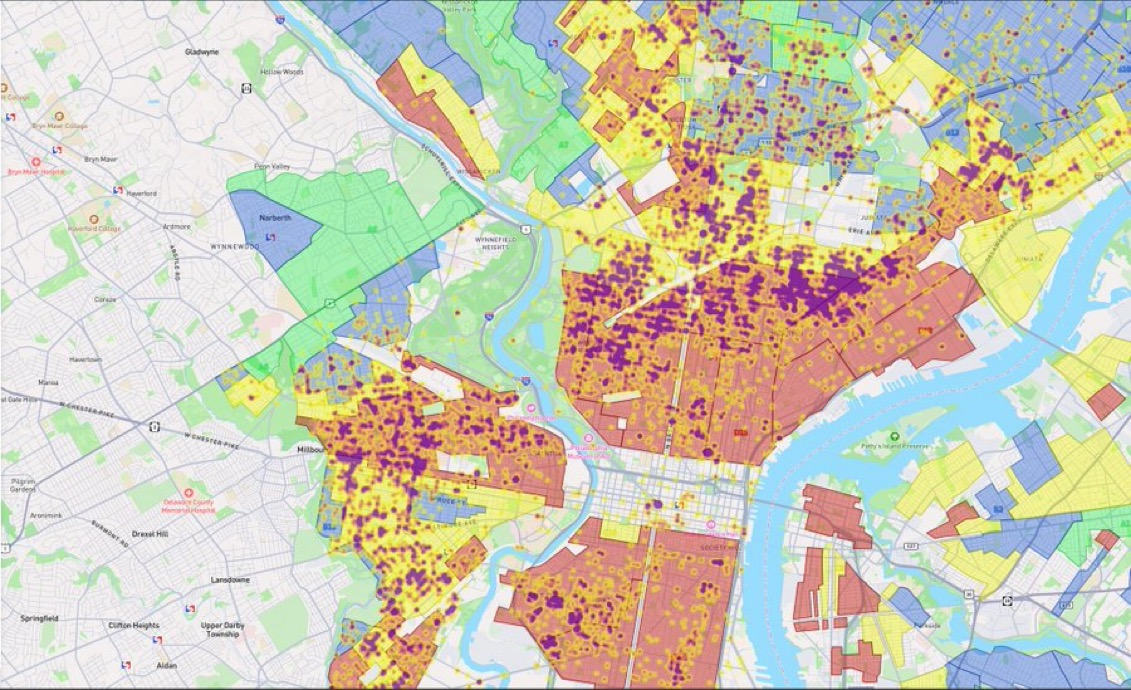
\includegraphics[width=\textwidth]{Philadelphia_gun_red.jpeg}
\caption{\textbf{Philadelphia: Contemporary Gun Homicides Overlaid on Historical HOLC Redlining Boundaries.} Purple/dark clusters represent modern gun homicide concentrations. The underlying color zones represent the 1930s HOLC grades: red (``Hazardous''), yellow (``Definitely Declining''), blue (``Still Desirable''), and green (``Best''). The spatial correlation is near-perfect: the sites of contemporary lethal violence map directly onto the zones that were systematically starved of capital nearly a century ago. The violence is not a cultural failure; it is the compounding output of $P_{\text{redlining}}$ applied to $O_{\text{racialized}}$.}
\label{fig:philly_redline}
\end{figure}

The Elite effectively trapped the Out-group in an environment of manufactured danger, maximizing their victimization while simultaneously removing the state's obligation to protect them. The gang violence used as the primary ideological justification for modern gun control is not a spontaneous failure of culture or a universal threat; it is the predictable, mathematical output of $P_{\text{redlining}}$ compounding over time. The system starves a zip code of capital, watches the poverty-crime correlation produce homicides, and then uses those homicides to justify stripping the constitutional autonomy of the entire population.

\subsection{``Mental Gun Control'' and the Threat of State Violence}
Having engineered this localized violence, the system required a mechanism to ensure the Out-group remained entirely defenseless against it. The Elite achieved this through the deployment of ``Mental Gun Control''---a profound psychological operation utilizing the framework's third component: Ideological Justification.

The system aggressively vilified Black firearm ownership through political rhetoric and media framing, associating it exclusively with gang violence, deviance, and criminality, rather than constitutional self-defense. The objective of this cultural programming was to condition the Out-group to fear and reject the very tools required for their own protection, effectively convincing them to disarm themselves.

Furthermore, when the psychological proxy fails and members of the Out-group attempt to legally arm themselves, the system reverts to absolute physical deterrence: police brutality. The state's enforcement algorithm is programmed to view a legally armed Black citizen not as a Second Amendment beneficiary, but as an immediate, lethal threat.

The 2016 police killing of Philando Castile serves as the definitive contemporary proof of this algorithm. Castile, a Black man who possessed a legal permit to carry a concealed weapon, informed the officer of his legally armed status during a routine traffic stop and was summarily executed in his vehicle. His death, and the subsequent acquittal of the officer, mathematically codified the system's unwritten rule: For the In-group ($I$), bearing arms is a protected liberty; for the Out-group ($O$), bearing arms is a capital offense.

Through the dual mechanisms of mental gun control and the constant threat of state violence, the Elite successfully maintains the Out-group's vulnerability. They are forced to live in engineered danger while being violently punished for attempting to defend themselves against it.

\subsection{Scaling the Algorithm: Pacification and Global Femicide}

The psychological operation defined as ``Mental Gun Control''---the conditioning of a subjugated group to fear and reject the very tools required to neutralize physical asymmetry---is not exclusively constrained to the axis of race. The systemic architecture of oppression is fractal; its core algorithms scale across different demographic categories to maintain various exploitable Out-groups.

The most devastating application of this psychological proxy outside of race is its weaponization against women. Across global societies, a deeply entrenched ideological narrative (Component~3) has been engineered to convince women of their inherent physical defenselessness while simultaneously conditioning them to reject the acquisition of lethal autonomy. Because firearms act as the ultimate mechanical equalizer of physical force---instantly neutralizing biological disparities in strength and size---the pacification of women is a necessary prerequisite for their systemic subjugation.

By utilizing cultural programming to convince this demographic to voluntarily disarm or reject self-defense technologies, the system mathematically engineers their vulnerability. The contemporary crisis of global femicide is not a spontaneous sociological tragedy; it is the predictable, mathematical output of asymmetrical disarmament. Just as the State disarmed $O_{\text{racialized}}$ to ensure unresisted extraction, patriarchal systems deploy Mental Gun Control to ensure that women remain physically vulnerable to both interpersonal and structural violence.

\subsection{The Modern Exploit: Redefining ``The People'' for Disarmament}

As the Demographic Paradox forces the Elite to cannibalize the Buffer Class, the original 1705 contract is actively being broken. Because $E$ is now subjecting members of $I_{\text{buffer}}$ to the extraction kernel, the Elite faces an existential threat: the Buffer Class still possesses the ``Physical Guarantee'' (the Second Amendment) they were issued centuries ago.

To prevent the inevitable violent revolt that occurs when a pacified class realizes it is being harvested, the Elite must rapidly recall the physical collateral. However, a blanket repeal of the Second Amendment would trigger immediate systemic collapse. Instead, the Elite actively exploits Constitutional Bug~\#1 (the undefined nature of ``We the People'').

Modern gun control operates not by banning the right itself, but by mathematically redefining the boundaries of the In-group. By intersecting arbitrary proxy variables with constitutional rights, the system can systematically excise individuals from ``the people.'' For example, both liberal and conservative political architectures currently utilize the federal criminalization of cannabis to strip Second Amendment rights from state-legal medical cannabis patients. The logic dictates that if an individual's status intersects with this variable ($\text{Status}(x) \cap P_{\text{cannabis}}$), they are instantaneously reclassified as latent criminals and excised from ``the people.''

Through these legislative exploits, the Elite successfully strips lethal autonomy from the population piecemeal, recalling the physical tools of revolution without ever openly declaring war on the Buffer Class.
\section{Universal Latent Criminality and Selective Enforcement}

As the Demographic Paradox (Section~6.2) forces the system to cannibalize $I_{\text{buffer}}$, the Elite faces a logistical hurdle: how do they transition the In-group into the carceral extraction pool without passing explicit laws that trigger a class revolt?

The solution, conceptualized by legal scholar Harvey Silverglate, is the mathematical expansion of the penal code to the point of ``Universal Latent Criminality.'' The modern legislative architecture is composed of an infinitely complex, overlapping web of vague statutes. Consequently, the average citizen unknowingly commits approximately three federal felonies a day.

The variable $P_{\text{criminal}}$ has expanded to encompass virtually the entire population. Therefore, what determines who enters the 13th Amendment carceral system is no longer the commission of a crime, but the \textit{Selective Enforcement} of the law by $F_{\text{enforce}}$. The Elite does not need to write new laws to enslave the Buffer Class; they simply direct the enforcement apparatus to selectively actuate the latent criminality already present in the In-group.


\section{The Full Reveal: The Complete 5-Tier Set-Theoretic Hierarchy}

Over the preceding four centuries of historical narrative, the reader has watched the Elite iteratively construct their extraction architecture---each tier invented as an emergency patch for a specific security vulnerability. We have now traced the construction of each tier through its historical moment of invention:

\begin{itemize}
    \item \textbf{The Elite ($E$)} and \textbf{the Out-group ($O_{\text{racialized}}$)}: invented in 15th-century Portugal to break the moral community and create an extractable labor class (Chapter~2).
    \item \textbf{The Buffer Class ($I_{\text{buffer}}$)}: originating in 15th-century Portugal---where the implicit contract first granted poor Europeans elevated status over racialized Africans (Chapter~2)---then formalized after Bacon's Rebellion (1676) to partition the working class and deploy the psychological wage $\psi$ (Chapter~3).
    \item \textbf{The Puppet Class ($P_{\text{uppet}}$)}: prototyped at the Constitutional Convention (1787), then industrialized through Tweedism in the Gilded Age, to separate the political front-end from the capital back-end (Chapters~3 and~5).
    \item \textbf{The Enforcement Class ($F_{\text{enforce}}$)}: evolved from slave patrols (1704) through the Fugitive Slave Act to modern policing, compensated with Qualified Immunity ($QI$) (Chapter~4).
\end{itemize}

For the first time, we can present the complete architecture as a unified hierarchy. The system is governed by what we term the \textbf{Predatory Min-Max Function}:

\begin{enumerate}
    \item \textbf{Maximize ($Max$):} The extraction of capital, labor, and autonomy from the labor force---primarily from $O_{\text{racialized}}$, but eventually from $I_{\text{buffer}}$ as well.
    \item \textbf{Minimize ($Min$):} The risk of a unified class revolution against the Elite ($E$), achieved by deploying $\psi$ to keep $I_{\text{buffer}}$ invested in racial hierarchy rather than class solidarity, $F_{\text{enforce}}$ invested through $QI$, and $P_{\text{uppet}}$ tethered through capital dependency.
\end{enumerate}

\[
\text{Objective:} \quad \frac{\text{Max}(\text{Extraction})}{\text{Min}(\text{Resistance}_{\text{class}})} \rightarrow \text{System Stability}
\]

The complete five-tiered inequality:
\[
\text{Benefit}(E) \gg \text{Benefit}(P_{\text{uppet}}) > \text{Benefit}(F_{\text{enforce}}) > \text{Benefit}(I_{\text{buffer}}) > \text{Benefit}(O_{\text{racialized}})
\]
where $\text{Benefit}(I_{\text{buffer}})$ consists primarily of $\psi$ (psychological wages), $\text{Benefit}(F_{\text{enforce}})$ consists of Qualified Immunity ($QI$), $\text{Benefit}(P_{\text{uppet}})$ consists of delegated political power tethered to $E$'s capital, and $\text{Benefit}(E)$ reflects the material wealth extracted from all tiers below.

\begin{figure}[htbp]
\centering
\begin{tikzpicture}[
    tier/.style={draw, thick, minimum height=0.9cm, align=center, font=\small},
    arr/.style={->, thick, >=stealth},
    scale=0.95, transform shape
]
    % Pyramid tiers (bottom to top)
    \node[tier, fill=red!30, minimum width=12cm] (t5) at (0,0)
        {\textbf{Tier 5: Out-group} ($O_{\text{racialized}}$) --- Primary extraction pool};
    \node[tier, fill=blue!15, minimum width=9.5cm] (t4) at (0,1.2)
        {\textbf{Tier 4: Buffer Class} ($I_{\text{buffer}}$) --- Pacified by $\psi$};
    \node[tier, fill=orange!25, minimum width=7cm] (t3) at (0,2.4)
        {\textbf{Tier 3: Enforcement} ($F_{\text{enforce}}$) --- $QI$};
    \node[tier, fill=purple!20, minimum width=5.5cm] (t2) at (0,3.6)
        {\textbf{Tier 2: Puppet Class} ($P_{\text{uppet}}$)};
    \node[tier, fill=green!40, minimum width=3.5cm] (t1) at (0,4.8)
        {\textbf{Tier 1: Elite} ($E$)};

    % Right-side benefit labels (anchored to right edge of each tier)
    \node[font=\scriptsize, green!60!black, anchor=west] at (t1.east) [xshift=0.3cm] {Material wealth (absolute)};
    \node[font=\scriptsize, purple!60, anchor=west] at (t2.east) [xshift=0.3cm] {Delegated power (conditional)};
    \node[font=\scriptsize, orange!70!black, anchor=west] at (t3.east) [xshift=0.3cm] {$QI$ (conditional)};
    \node[font=\scriptsize, blue!70, anchor=west] at (t4.east) [xshift=0.3cm] {Psychological wage $\psi$};
    \node[font=\scriptsize, red!70, anchor=west] at (t5.east) [xshift=0.3cm] {Extraction};

    % Left-side extraction arrow
    \draw[arr, very thick, red!60] (-6.8,4.5) -- (-6.8,0.3);
    \node[font=\scriptsize, red!60, rotate=90] at (-7.3,2.4) {Extraction flows upward};

    % Left-side control arrow
    \draw[arr, very thick, gray] (-5.8,0.3) -- (-5.8,4.5);
    \node[font=\scriptsize, gray, rotate=90] at (-5.3,2.4) {Control flows downward};

    % Bottom annotation
    \node[font=\scriptsize, align=center, gray] at (0,-0.9) {The Elite does not govern or enforce directly---each tier insulates $E$ from visibility and consequence.};
\end{tikzpicture}
\caption{\textbf{The 5-Tier Set-Theoretic Hierarchy.} The system is organized as a layered pyramid of extraction. Control flows downward from the Elite through the Puppet Class and Enforcement Class, while extracted wealth flows upward. Each intermediate tier receives a conditional benefit (delegated power, legal immunity, psychological wages) calibrated to ensure compliance. The Out-group bears the primary compounding burden of extraction.}
\label{fig:elite_model}
\end{figure}

This five-tier structure is governed by what we term the \textbf{Predatory Min-Max Function}. The system operates according to two imperatives:

\begin{enumerate}
    \item \textbf{Maximize ($Max$):} The extraction of capital, labor, and autonomy from the labor force---primarily from $O_{\text{racialized}}$, but eventually from $I_{\text{buffer}}$ as well.
    \item \textbf{Minimize ($Min$):} The risk of a unified class revolution against the Elite ($E$), achieved by deploying $\psi$ to keep $I_{\text{buffer}}$ invested in racial hierarchy rather than class solidarity, $F_{\text{enforce}}$ invested through $QI$, and $P_{\text{uppet}}$ tethered through capital dependency.
\end{enumerate}

\[
\text{Objective:} \quad \frac{\text{Max}(\text{Extraction})}{\text{Min}(\text{Resistance}_{\text{class}})} \rightarrow \text{System Stability}
\]

Policies ($P$) are the instruments through which this optimization is executed, impacting each tier in structurally different ways. $P_{\text{uppet}}$ writes the policies, $F_{\text{enforce}}$ actuates them, $I_{\text{buffer}}$ is pacified into accepting them, and $O_{\text{racialized}}$ bears the compounding burden. The remainder of this section formalizes how these policies compound over time; the preceding chapters have traced the historical algorithm of Elite optimization through its successive phases.
\section{The Collapse: Cannibalizing the In-Group (Present)}
This brings us to the final, inevitable stage of the algorithm. An extraction system requires \textbf{Infinite Growth}. Once the Out-group ($O$) has been fully harvested---stripped of wealth, voting rights, and labor \cite{coates}---the Elite ($E$) must find new sources of extraction to maintain their accumulation.

The system has now turned inward. The tools developed to oppress the Out-group are being deployed against the In-group:
\begin{itemize}
    \item \textbf{The Opioid Crisis:} The criminalization of white addiction mirrors the crack epidemic.
    \item \textbf{Militarized Policing:} SWAT tactics invented for the "Ghetto" are now used in rural towns.
    \item \textbf{Surveillance:} The loss of privacy tested on the poor is now applied to the middle class.
\end{itemize}

The expansion of $O$ is facilitated by a structural development that legal scholar Harvey Silverglate identifies: the average American now unknowingly commits approximately \textbf{three federal felonies per day} \cite{silverglate}. The proliferation of vague, overlapping, and over-broad criminal statutes---combined with prosecutorial discretion in charging---means that the proxy variable $P$ has become \textit{omnipresent}. Nearly every citizen is technically criminal; what determines who enters the carceral system is not the commission of crime but the \textit{selection} of targets. This transforms the system's primary mechanism from demographic targeting to \textbf{selective enforcement}: the Elite no longer needs to define the Out-group explicitly, because the criminalization kernel ($\text{If } \text{Status}(x) = \text{Criminal}(C) \rightarrow \text{Status}(x) \in S$) can now reach \textit{anyone}. ``Broken windows'' policing \cite{wilson} and its progeny provide the discretionary framework---the theoretical justification for intensive policing of minor infractions---while the empirical evidence shows that such policing is deployed overwhelmingly in communities already marked by the compounding chain of Section~4.5 \cite{harcourt}. The system has thus achieved what might be called \textbf{universal latent criminality}: the entire population exists in a state of potential subjugation, with actual subjugation determined by $E$'s extraction needs.

\section{The Recursive Extraction Engine: Biological Degradation as Control}

To fully comprehend the Elite subset’s ($E$) control matrix, the analysis must expand beyond legal and labor extraction to include the deliberate manipulation of the population's biological autonomy. The contemporary Medical-Industrial Complex (MIC) and the subsidized agricultural sector do not operate independently; they function as a unified, recursive extraction algorithm.

Within this framework, the system is designed to transition the population from a state of symmetrical biological autonomy ($O_{\text{full\_capacity}}$) into a state of chronic, manageable illness ($O_{\text{degraded}}$). A biologically compromised population serves a dual function for the Elite: it generates infinite, recurring revenue, and it physiologically neutralizes the capacity for class resistance \cite{washington}.

\subsection{Phase 1: The Toxin Variable (\texorpdfstring{$P_{\text{toxin}}$}{P\_toxin}) and the "Affordability Trap"}

The extraction loop begins with the engineered degradation of the food supply. The system utilizes seemingly neutral economic policies ($P$)—specifically agricultural subsidies and a reversed regulatory framework (such as the FDA's "Generally Recognized as Safe" or GRAS loophole, which allows manufacturers to self-regulate)—to flood the market with high-fructose corn syrup, refined grains, and chemical additives. Currently, nearly 70\% of packaged foods in the U.S. are classified as ultra-processed, supplying more than half of adults' daily calories.

This is not an accident of the free market; it is a meticulously engineered "Affordability Trap" designed to aggressively target the Out-group ($O$) and the lower-tier Buffer Class ($I \setminus E$). A 2026 comprehensive audit by Harvard Law School’s Food Law and Policy Clinic mathematically proved that price strictly dictates a population's exposure to toxicity.
The study revealed a stark biological matrix:
\begin{itemize}
    \item \textbf{The Additive Multiplier}: The lowest-priced food products contain, on average, 2.6 times more additives than the most expensive options (averaging 6.6 additives per item versus 2.7).
    \item \textbf{High-Risk Concentration}: In staple categories, the disparity accelerates. The cheapest store-bought breads contain nearly 4 times more additives, and the cheapest frozen pizzas contain an average of 12 additives per product (compared to 4.4 in the highest tier). Most critically, the cheapest products contain over 3 times more high-risk, health-compromising additives.
    \item \textbf{The Caloric Payload}: Lower-priced foods are engineered to be chemically addictive and physiologically destructive, containing 21\% more sugar and 10\% more sodium than their higher-priced counterparts.
\end{itemize}
To maintain baseline biological autonomy—meaning, to consume products free of high-risk additives—a consumer must pay an average price premium of 63\%.

Within the Predatory Min-Max Function, this 63\% premium functions as a biological poll tax. The Elite class ($E$) sets the financial threshold for physical health intentionally out of reach for the Out-group ($O$), forcing them to consume the very toxins that will push them into the $O_{\text{degraded}}$ state. By making optimal nutrition artificially expensive and toxic food artificially cheap, the system mathematically guarantees the mass onset of chronic conditions such as obesity, hypertension, and Type 2 diabetes. The Out-group is not "choosing" a poor diet; they are being economically confined to a designated toxicity zone.

\section{The Cannibalization of the Buffer Class and the Endpoint of the Algorithm}

The "White Working Class" was never a partner to the Elite; they were merely the \textbf{Reserve Food Supply}. By accepting the bribe of "Whiteness" in 1705, they agreed to police the prison that is now expanding to hold \textit{them}. The terminal phase of the extraction algorithm is characterized by the system turning inward. A fundamental theorem of the Predatory Min-Max Function is that the Elite ($E$) possesses no permanent loyalty to the Buffer Class ($I \setminus E$). The baseline privileges afforded to the In-group—such as Second Amendment protections and presumptions of innocence—are not inherent rights; they are conditional algorithmic variables used to maintain systemic stability. As the Elite's demand for absolute control intensifies, the algorithm inevitably begins cannibalizing its own defenders. The boundary of the Out-group ($O$) expands outward to subsume the In-group.

The ultimate, devastating proof of this terminal phase is the 2026 killing of Alex Perdi by Immigration and Customs Enforcement (ICE) agents. Demographically, as a cisgender white man, Perdi represented the historical core of the protected Buffer Class. Under the ideological justification (Component 3) of the Second Amendment, his decision to arm himself in confrontation with law enforcement should theoretically have been shielded by the same "anti-tyranny" constitutional interpretations routinely afforded to the In-group.

\subsection{Disarmament and Execution: The Algorithm Unmasked}
However, the reality of the encounter proved that the system's operational code has shifted. During the confrontation, Perdi was successfully disarmed. At the exact moment he lost his lethal autonomy, he ceased to be a member of the protected class. He was no longer treated as a citizen possessing constitutional rights; the state enforcement algorithm immediately reclassified him as a neutralized biological asset and executed him.

This event mathematically shatters the core illusion of the American operating system. It demonstrates that the state's enforcement apparatus—originally designed as slave patrols to violently manage the racialized Out-group—has now been fully authorized to deploy lethal extraction against anyone outside of the true Elite ($E$), regardless of their demographic status.

The execution of a disarmed white citizen by federal agents proves that the "wages of whiteness" are effectively bankrupt. The Second Amendment does not protect the Buffer Class from state violence; it merely serves as a temporary pacifier until the state decides to revoke it. The system has reached its most optimized, terrifying state: a pure binary where absolute immunity is reserved exclusively for the Elite ($E$), and every other citizen is mathematically confined to the Out-group, waiting to be harvested.

The definition of the Out-group has returned to its 1676 state:

\[
O_{final} = \text{Everyone} \setminus E
\]

\begin{figure}[h]
    \centering
    \begin{tikzpicture}[scale=0.88, every node/.style={font=\small}]

    % --- Phase 1: 1676 (United labor) ---
    \begin{scope}[shift={(0,0)}]
        \node[font=\footnotesize\bfseries, anchor=south] at (1.5,2.85) {1676: Unity};
        % Elite box
        \draw[thick, green!60!black, fill=green!40] (0.8,1.8) rectangle (2.2,2.6);
        \node[green!60!black, font=\scriptsize] at (1.5,2.2) {$E$};
        % United labor
        \draw[thick, purple!70, fill=purple!20] (0,0) rectangle (3,1.5);
        \node[purple!70, font=\scriptsize, align=center] at (1.5,0.75) {$L_{white} \cup L_{black}$\\(United Labor)};
        % Threat arrow
        \draw[->, very thick, red!70] (1.5,1.5) -- (1.5,1.8);
        \node[red!70, font=\tiny, rotate=90] at (0.3,1.65) {Threat};
    \end{scope}

    % Arrow
    \draw[->, very thick, gray] (3.3,1.2) -- (4.0,1.2);

    % --- Phase 2: 1705 (Partition) ---
    \begin{scope}[shift={(4.3,0)}]
        \node[font=\footnotesize\bfseries, anchor=south] at (1.5,2.85) {1705: Partition};
        % Elite box
        \draw[thick, green!60!black, fill=green!40] (0.8,1.8) rectangle (2.2,2.6);
        \node[green!60!black, font=\scriptsize] at (1.5,2.2) {$E$};
        % Buffer class (white)
        \draw[thick, blue!70, fill=blue!15] (0,0.8) rectangle (3,1.5);
        \node[blue!70, font=\scriptsize] at (1.5,1.15) {$I_{poor}$ (Buffer)};
        % Extraction zone (black)
        \draw[thick, red!80, fill=red!30] (0,0) rectangle (3,0.65);
        \node[red!80, font=\scriptsize] at (1.5,0.32) {$O$ (Enslaved)};
        % Shield arrow
        \draw[->, thick, blue!70] (1.5,1.5) -- (1.5,1.8);
        \node[blue!70, font=\tiny, rotate=90] at (0.3,1.65) {Shield};
    \end{scope}

    % Arrow
    \draw[->, very thick, gray] (7.6,1.2) -- (8.3,1.2);

    % --- Phase 3: 1865--1968 (Expansion) ---
    \begin{scope}[shift={(8.6,0)}]
        \node[font=\footnotesize\bfseries, anchor=south] at (1.5,2.85) {1865--1968};
        % Elite box
        \draw[thick, green!60!black, fill=green!40] (0.8,1.8) rectangle (2.2,2.6);
        \node[green!60!black, font=\scriptsize] at (1.5,2.2) {$E$};
        % Buffer class (shrinking)
        \draw[thick, blue!70, fill=blue!15] (0,1.1) rectangle (3,1.5);
        \node[blue!70, font=\scriptsize] at (1.5,1.3) {Buffer (shrinking)};
        % Expanded extraction zone
        \draw[thick, red!80, fill=red!30] (0,0) rectangle (3,0.95);
        \node[red!80, font=\scriptsize, align=center] at (1.5,0.48) {$O$ + Criminals\\+ Drug Users};
    \end{scope}

    % Arrow
    \draw[->, very thick, gray] (11.9,1.2) -- (12.6,1.2);

    % --- Phase 4: Present (Cannibalization) ---
    \begin{scope}[shift={(12.9,0)}]
        \node[font=\footnotesize\bfseries, anchor=south] at (1.5,2.85) {Present};
        % Elite box
        \draw[thick, green!60!black, fill=green!40] (0.8,1.8) rectangle (2.2,2.6);
        \node[green!60!black, font=\scriptsize] at (1.5,2.2) {$E$};
        % Extraction zone consuming nearly everything
        \draw[thick, red!80, fill=red!30] (0,0) rectangle (3,1.5);
        \node[red!80, font=\scriptsize, align=center] at (1.5,0.75) {$O_{final}$\\$= \text{Everyone} \setminus E$};
        % Cannibalization arrow
        \draw[->, very thick, red!80, dashed] (1.5,1.5) -- (1.5,1.8);
        \node[red!80, font=\tiny, rotate=90] at (0.15,1.65) {Threat};
    \end{scope}

    % Bottom annotation
    \draw[->, very thick, red!60] (0,-0.5) -- (15.9,-0.5);
    \node[red!60, font=\footnotesize, anchor=west] at (4.5,-0.9) {Extraction zone expands $\longrightarrow$ Buffer consumed};

    \end{tikzpicture}
    \caption{\textbf{The Recursive Expansion of the Extraction Zone (1676--Present).} This diagram illustrates the ``Min-Max'' algorithm in motion. Following the threat of unity in 1676, the Elite created a racial partition to separate the labor force. However, as the extraction system requires infinite growth, the ``Out-group'' ($O$) has progressively expanded---first capturing Black bodies via chattel slavery, then criminalized populations via the War on Drugs, and finally cannibalizing the white working class via the modern surveillance and opioid crises. The ``Buffer Class'' ($I$) was never a permanent partner to the Elite, but a temporary reserve of capital.}
    \label{fig:extraction_zone}
\end{figure}
\section{The Stress Test: The Epstein Network and Elite Immunity}

The framework's predictive power can be evaluated against a contemporary case that tests its central claims about Elite immunity from the carceral state. The network surrounding Jeffrey Epstein---whose trafficking operation implicated figures across finance, politics, and academia---provides a devastating stress test. The model predicts that members of $E$ will be shielded from the very carceral mechanisms that the system deploys against $O_{\text{racialized}}$ and, increasingly, against $I \setminus E$. The Epstein case confirms this prediction at every level.

First, the \textit{duration and visibility of impunity}: despite complaints to law enforcement dating to the early 2000s, the initial federal prosecution in 2008 resulted in a non-prosecution agreement that granted immunity to unnamed co-conspirators---an outcome functionally unavailable to defendants outside $E$. Second, the \textit{institutional protection mechanisms}: following the passage of the Epstein Files Transparency Act \cite{epsteinact}---bipartisan legislation mandating disclosure of federal records related to the case---the disclosed materials revealed that agencies tasked with enforcement had possessed substantial evidence for years without pursuing charges against network participants who occupied positions within $E$. The disclosure process itself became contested: members of Congress reviewing the materials reported surveillance by federal agencies, suggesting that the institutional apparatus designed to enforce law was instead deployed to monitor those investigating Elite conduct. In February 2026, United Nations human rights experts characterized the pattern of obstructed accountability as ``institutional gaslighting''---a term that maps precisely onto Component~4 of the oppressive architecture (resistance to structural critique) \cite{ohchr2026}.

Third, and most relevant to the model's financial architecture, firms connected to network participants---including Apollo Global Management, whose former CEO's extensive contacts with Epstein were documented in the disclosed files---continued to operate without regulatory consequence, with the firm's assets under management growing to over \$700 billion \cite{apolloepstein}. This mirrors the unbroken financial lineage identified in Section~2.5: just as antebellum banks that securitized enslaved bodies became predecessor institutions of modern financial giants, contemporary financial entities connected to documented exploitation face no structural accountability. The carceral state that processes millions of $O_{\text{racialized}}$ and $I \setminus E$ members annually for minor infractions proves structurally incapable of reaching $E$, even when the conduct in question involves the gravest offenses against the most vulnerable. The Epstein case does not merely illustrate Elite immunity---it demonstrates that the Predatory Min-Max Function's asymmetry extends to the most extreme domains: the same system that imprisons citizens for possessing cannabis (Section~6.1) cannot hold accountable those within $E$ whose offenses are orders of magnitude more severe.

\section{The Failure of the \texorpdfstring{$Min$}{Min} Variable and the Disarmament Panic}

This cannibalization of the Buffer Class brings the Predatory Min-Max Function to its terminal crisis point. By subjecting $I_{\text{buffer}}$ to the extraction kernel---through the opioid crisis, the affordability trap, and selective carceral enforcement---the Elite is actively violating the foundational 1705 contract.

Because the contract is broken, the $Min$ variable (the minimization of class resistance) is failing severely. The Buffer Class is beginning to realize that the ``wages of whiteness'' are bankrupt and that they are merely the system's reserve food supply. This creates a terrifying reality for $E$: the betrayed In-group still possesses the ``Physical Guarantee'' (the Second Amendment) they were issued centuries ago.

This failing $Min$ variable is the true algorithmic driver behind the modern panic for sweeping disarmament. The aggressive push by political structures to ban common-use firearms---such as the expansive 2026 legislation passed by the Virginia General Assembly---is not an exercise in public safety. It is the Elite acting out of sheer systemic terror. Knowing that their breach of contract makes a violent class revolt mathematically inevitable, $E$ is deploying $P_{\text{uppet}}$ to desperately recall the physical collateral before the In-group can turn their weapons against the architects of the extraction engine.

\subsection{The Kinetic Calculus: The Mathematical Scale of the Civilian Threat}

To fully comprehend the systemic terror driving the Elite's ($E$) disarmament protocols, we must quantify the actual kinetic capacity of the population they are attempting to subjugate. The system relies on the assumption that the Enforcement Class ($F_{\text{enforce}}$) possesses overwhelming physical superiority. However, a mathematical audit of the physical hardware reveals a catastrophic vulnerability in the extraction engine.

The American civilian class is not merely well-armed; it is the most heavily armed entity in human history. With an estimated 400 million small arms in civilian hands, this demographic possesses more firepower than all the world's militaries combined.

Critically, this figure---derived from manufacturing records, import/export data, and survey estimates---represents only the \textit{reported} count: firearms that passed through the formal commercial pipeline and left a traceable paper trail. It does not account for privately manufactured firearms built by lawful citizens who exercised their legal right to produce arms for personal use without serialization or registration---a practice the system is now retroactively criminalizing, as the Dexter Taylor case demonstrates (Section~\ref{sec:dexter_taylor}). Nor does it account for the vast underground arms economy: stolen, trafficked, and informally circulated weapons that exist entirely outside the state's surveillance architecture. The true number of functional firearms in civilian hands is, by mathematical necessity, substantially higher than 400 million---a reality that makes the Elite's kinetic deficit even more catastrophic than the official estimate suggests.

Within the framework, the total kinetic power of the non-Elite population can be mapped as:

\[
\text{Kinetic}(I_{\text{buffer}} \cup O_{\text{racialized}} \setminus O_{\text{incarcerated}}) \gg \text{Kinetic}(F_{\text{enforce}} \cup E)
\]

This equation represents the ultimate failure of the $Min$ variable. The Elite has spent centuries mathematically engineering a system to extract wealth from a population that currently possesses the physical capacity to dismantle the entire enforcement apparatus overnight.

\subsubsection*{The Legal Filter vs.\ Physical Reality}

The Elite attempts to manage this overwhelming kinetic disadvantage through the legislative proxy of criminalization ($P_{\text{criminal}}$). By intersecting constitutional rights with felony statutes, the system attempts to mathematically subtract individuals from the armed pool.

However, this creates a profound structural illusion. While a felony conviction legally strips a citizen of their Second Amendment status---officially transferring them into the disarmed Out-group ($O_{\text{degraded}}$)---it does not instantly alter physical reality. As long as these individuals are not actively caged within the carceral state ($O_{\text{incarcerated}}$), many retain access to physical hardware through the informal economy.

This generates a ``rogue variable'' within the system: an expanding class of heavily armed individuals who have already been legally and economically annihilated by the state, and therefore have nothing left to lose.

For the Elite, this is the nightmare scenario. They are attempting to cannibalize a Buffer Class ($I_{\text{buffer}}$) that holds world-historical levels of firepower, while simultaneously expanding a criminalized Out-group ($O$) that ignores the legal parameters of disarmament altogether. The frantic push by $P_{\text{uppet}}$ to ban hardware, construct financial barriers, and impose universal latent criminality is not a sign of the system's strength; it is a desperate, flailing response to the mathematical reality that the Elite is kinetically outnumbered, outgunned, and running out of ideological shields.

\section{Live Execution of the Code: The 18~U.S.C.~\S922(g)(3) Crisis}

The theoretical framework of Universal Latent Criminality and the exploitation of Constitutional Bug~\#1 (the undefined parameters of ``We the People'') is not merely historical; it is actively being litigated by the Judicial Shield ($P_{\text{uppet}}$) in real time. The 2026 Supreme Court arguments regarding 18~U.S.C.~\S922(g)(3)---which permanently strips the Second Amendment ``Physical Guarantee'' from anyone deemed an ``unlawful user'' of a controlled substance---serve as a pristine, live-action diagnostic of the Elite's disarmament algorithm.

During oral arguments in \textit{United States v.\ Hemani} (2026), the underlying mechanics of systemic extraction were laid bare. The government argued that intersection with the Controlled Substances Act acts as an automatic proxy for ``dangerousness,'' justifying total revocation of constitutional autonomy. To satisfy the historical requirements of the \textit{Bruen} doctrine, the state attempted an algorithmic ``Interface Swap,'' arguing that modern cannabis users are the legal equivalent of 18th-century ``habitual drunkards'' and vagrants---classes historically targeted for forced labor and civil death.

However, the sheer breadth of the statute exposed the reality of Universal Latent Criminality. As the Justices noted, the government's strict interpretation means that a citizen who unlawfully takes a spouse's prescription sleep aid (Ambien) or a roommate's study medication (Adderall) is mathematically identical to a violent felon, rendering them permanently disarmed.

The state's defense of this overreach perfectly encapsulates the mechanics of Selective Enforcement. The Elite does not intend to permanently disarm the suburban professional taking an unprescribed Ambien; the system relies on the fact that the statute is broad enough to make everyone a latent felon. The Enforcement Class ($F_{\text{enforce}}$) is then entrusted to selectively aim this legal weapon, filtering who gets to remain in the Buffer Class and who gets stripped of their physical collateral and dropped into the carceral Out-group.

The \S922(g)(3) litigation is the ultimate proof that the Elite does not need to formally rewrite the Constitution to revoke the 1705 contract. By expanding the definition of $P_{\text{criminal}}$ through the bureaucratic scheduling of substances, the system quietly and continuously shrinks the definition of ``We the People,'' executing a silent, algorithmic disarmament of the populace before the $Min$ variable completely fails.

\section{The Geopolitical Override: The ``Deep State'' and Manufactured Crisis}

To understand the ultimate defensive capabilities of the Predatory Min-Max Function, we must examine how the system reacts when the true Elite ($E$) faces an existential threat of exposure that cannot be contained by standard domestic algorithms.

The catastrophic release of the Epstein files in 2025 and 2026 represented a critical system failure. For the first time, the mechanics of Elite systemic immunity---and the complicity of the Puppet Class ($P_{\text{uppet}}$)---were made visible to the Buffer Class ($I_{\text{buffer}}$). When domestic distractions and algorithmic corrections fail to pacify the population, the system activates its ultimate fail-safe: the \textbf{Geopolitical Override}.

Political scientist Aaron Good defines the ``Deep State'' not as a shadowy conspiracy, but as the permanent, unelected institutional architecture of imperial capital---the intelligence agencies, military-industrial contractors, and high finance sectors that operate independently of democratic input \cite{good}. In our set-theoretic framework, the Deep State represents the structural bedrock of $P_{\text{uppet}}$ and the command layer of the Enforcement Class ($F_{\text{enforce}}$).

Given this architecture, the model generates a specific prediction: when domestic exposure of $E$ reaches a critical threshold that cannot be contained by standard algorithmic corrections, the system will activate a Geopolitical Override---initiating kinetic foreign conflict to protect the domestic kernel. The 2026 Iran conflict exhibits precisely these predicted characteristics. As noted by contemporary geopolitical analysts, the war was launched with an anomalous ``paucity of pretext.'' The Predatory Min-Max Function provides the missing pretext: it was entirely internal. The temporal correlation between the Epstein file releases and the initiation of military operations is consistent with the Override function the model predicts.

The initiation of kinetic foreign conflict serves three vital mathematical functions for the Elite during a domestic crisis:

\begin{enumerate}
    \item \textbf{Information Saturation:} It immediately monopolizes the media and political ``Interface,'' burying the catastrophic domestic exposure (the Epstein files) under the urgent, life-or-death optics of global war.

    \item \textbf{The Redirection of Animus:} It weaponizes the $Min$ variable by giving the enraged Buffer Class a new, foreign Out-group ($O_{\text{foreign}}$) to fear and hate, successfully redirecting their kinetic anger away from the domestic Elite.

    \item \textbf{The Justification of Exceptionalism:} A state of war automatically justifies the suspension of transparency and the invocation of ``national security,'' allowing the institutional apparatus to close ranks, classify information, and protect compromised members of $E$ under the guise of patriotism.
\end{enumerate}

Whether the Iran conflict was consciously triggered by the Epstein exposure or represents a convergence of independent imperial interests is, within the framework, ultimately immaterial. The structural outcome is identical: the Military-Industrial Complex functions as the ultimate domestic shield. If the model's architecture is correct, $E$ will readily deploy $F_{\text{enforce}}$ to destabilize the globe whenever doing so creates the necessary geopolitical noise to prevent the Buffer Class from recognizing the extraction engine operating in their own backyards. The Iran--Epstein temporal alignment is either a deliberate activation of the Geopolitical Override or a demonstration that the system's incentive structure produces the same outcome without requiring conscious coordination---a distinction without a mathematical difference.

\chapter{The Disarmament Timeline: Gun Control as a Pillar of the Extraction Kernel}

\begin{tcolorbox}[colback=black!5, colframe=black!70, fonttitle=\bfseries\ttfamily, title=RUNTIME LOG: TRACING THE DISARMAMENT VARIABLE ACROSS THE FULL TIMELINE]
\ttfamily\small
\textbf{System Origin}: Portuguese firearms superiority (1440s) --- technological asymmetry in lethal capacity enables mass extraction.\\
\textbf{Feedback Loop Detected}: Arms-for-slaves trade creates exponential demand. Firearms $\rightarrow$ military advantage $\rightarrow$ captives $\rightarrow$ currency for more firearms.\\
\textbf{Constitutional Encoding}: Second Amendment (1791) --- kinetic guarantee installed as dead man's switch. Racial and gendered exclusions baked into source code.\\
\textbf{Disarmament Protocol}: NFA (1934) $\rightarrow$ Mulford Act (1967) $\rightarrow$ GCA (1968) $\rightarrow$ Hughes Amendment (1986) $\rightarrow$ Brady/AWB (1993--94) $\rightarrow$ Post-Bruen state responses (2022--present).\\
\textbf{PATTERN}: Every federal gun control law correlates with either (a) $O_{\text{racialized}}$ approaching kinetic parity or (b) $P_{\text{uppet}}$ members being kinetically corrected. The disarmament variable is not a policy debate---it is a \textbf{pillar} of the extraction kernel.
\end{tcolorbox}

\medskip

The preceding chapters have traced the Predatory Min-Max Function through its legal, economic, spatial, and psychological variables. But the framework has not yet isolated the variable that \textit{precedes all others}---the one without which the entire five-century extraction apparatus could not have been initialized. That variable is \textbf{asymmetric lethal capacity}: the technological gap in the ability to inflict organized violence.

Every extraction system documented in this book---chattel slavery, convict leasing, redlining, the carceral state---depends on the same precondition: the extracting class must possess a monopoly, or near-monopoly, on the capacity to kill. If the extracted population can fight back with equivalent force, the extraction equation collapses. The entire history of gun control in America---from the colonial era to the post-Bruen state responses of 2025---is the history of the Elite managing this single variable.

This chapter traces the disarmament variable from its origin to the present day, demonstrating that ``gun control'' is not a modern policy debate about public safety. It is a continuous, five-century operation to maintain the lethal asymmetry without which the Predatory Min-Max Function cannot execute.

\section{The Firearms Asymmetry: How Guns Created the African Diaspora}

The African diaspora exists outside Africa \textit{because of guns}.

This claim requires substantiation, but the historical record is unambiguous. When Portuguese traders first made contact with West African kingdoms in the mid-15th century, the technological gap in military capacity was decisive. European firearms---crude by later standards but devastating against populations that had not developed gunpowder weapons---provided the asymmetric lethal advantage that enabled mass kidnapping and, eventually, the transatlantic slave trade \cite{thornton}.

The extraction operated in two phases.

\subsection{Phase 1: Direct Kidnapping Through Firearms Superiority}

The earliest Portuguese slave raids on the West African coast relied on a simple calculus: a small number of armed men with firearms could overpower a larger number of defenders wielding edged and projectile weapons that could not match the range, lethality, or psychological impact of gunfire. This technological asymmetry---not racial superiority, not cultural destiny, not divine mandate---was the \textit{enabling condition} for the transatlantic slave trade. Without the gun, the extraction pipeline could not have been initialized.

The framework's notation captures this precisely. Let $L_E$ denote the lethal capacity of the Elite and $L_O$ the lethal capacity of the target population. The extraction precondition is:
\[
L_E \gg L_O \implies \text{Extraction feasible}
\]

When this inequality holds, $E$ can impose the full oppressive architecture: asymmetric power (Component~1), resource extraction (Component~2), ideological justification (Component~3), and resistance suppression (Component~4). When $L_O \to L_E$---when the target population approaches lethal parity---the extraction equation destabilizes. The entire history of gun control is the history of maintaining the inequality $L_E \gg L_O$ after the initial technological gap began to close.

\subsection{Phase 2: The Arms-for-Slaves Feedback Loop}

The second phase was more insidious---and more profitable. As the slave trade matured, the Portuguese and subsequently the Dutch, British, and French discovered that they could \textit{weaponize the firearms asymmetry itself} as a currency system. European traders sold firearms to coastal African kingdoms, but the only currency they accepted in return was enslaved human beings \cite{inikori}.

This created an exponential feedback loop:

\begin{enumerate}
    \item European traders introduce firearms to Kingdom A.
    \item Kingdom A now possesses a decisive military advantage over neighboring Kingdom B.
    \item Kingdom B faces a choice: acquire firearms or be conquered and enslaved.
    \item The only way to acquire firearms is to provide enslaved people to the European traders.
    \item Kingdom B begins raiding Kingdom C to acquire captives to trade for firearms.
    \item The cycle propagates inland, creating an expanding wave of militarized slaving that reaches hundreds of miles from the coast.
\end{enumerate}

The mathematics are self-reinforcing. Once a single node in the system acquires firearms, every adjacent node must acquire them for defensive purposes. The only available currency is human bodies. The European Elite controlled the supply of firearms and the demand for slaves---they were both the arms dealer and the slave buyer, sitting at the apex of a system that forced African kingdoms into a coercive arms race whose fuel was their own population.

By the late 18th century, European traders were importing an estimated 283,000 to 394,000 firearms per year into West Africa, and the correlation between firearms imports and slave exports was direct and measurable \cite{inikori}. The feedback loop had achieved industrial scale.

\subsection{Dismantling the ``Africans Sold Themselves'' Counter-Argument}

The framework must address this counter-argument directly, because it is a pristine instantiation of $P_{\text{gaslight}}$ operating at civilizational scale.

The claim that ``Africans sold themselves into slavery'' requires the listener to perform the following cognitive operations:

\begin{enumerate}
    \item \textbf{Erase the coercive structure.} The arms-for-slaves dynamic was not a free market. Once European firearms entered the system, participation was not optional. A kingdom that refused to trade slaves for guns would be conquered by a kingdom that did. The ``choice'' to participate was the same ``choice'' a person makes when handing over their wallet at gunpoint.

    \item \textbf{Equate fundamentally different systems.} Pre-existing forms of servitude in West African societies---war captives, debt bondage, household labor---bore no structural resemblance to chattel slavery in the Americas. These were not hereditary, not racialized, not defined by the legal fiction that a human being is moveable property. The tribes who traded captives to European slavers did not know---and could not have anticipated---the industrial death machine of the Middle Passage and the plantation system \cite{smallwood}. Equating African domestic servitude with New World chattel slavery is like equating a bar fight with the atomic bomb because both involve violence.

    \item \textbf{Assign co-architect status to coerced participants.} The European Elite created the demand for slaves, supplied the firearms that coerced participation, built the ships, designed the plantation system, wrote the slave codes, and captured the profits. African kingdoms were \textit{nodes} in a system engineered by $E$, not co-architects of it. Blaming the coerced participants for the system that coerced them is the same logical operation as blaming the modern Out-group for the compounding effects of policies they had no hand in designing---which is precisely what $P_{\text{gaslight}}$ does domestically.
\end{enumerate}

The ``Africans sold themselves'' argument is not a historical correction. It is $P_{\text{gaslight}}^{\text{kernel denial}}$ applied retroactively to the origin point of the entire extraction system---an attempt to distribute the moral burden of the slave trade across its victims in order to dilute the causal responsibility of the Elite who engineered it.

\section{The Constitutional Encoding: The Second Amendment as Kinetic Guarantee (1791)}

Chapter~8's analysis of the Framers' twenty-one confessions established that the Second Amendment was designed as a dead man's switch---a permanent kinetic guarantee ensuring that the governed retain the physical capacity to terminate the constitutional contract by force. The Framers understood, because they had just fought a revolution triggered by a disarmament attempt, that every other right in the Bill of Rights depends on the population's ability to enforce those rights through lethal capacity.

But the constitutional source code contained two critical bugs from inception.

\textbf{Bug 1: The Racial Exclusion.} The Second Amendment protects ``the right of the people''---but as the Dred Scott decision would later make explicit, Black Americans were not included in ``the people.'' The kinetic guarantee was designed to protect the Buffer Class and the white population generally; the racialized Out-group was excluded by design. This is not a failure of the amendment---it is a feature of the extraction kernel. The system requires $L_E \gg L_O$; granting the Out-group lethal parity would collapse the extraction equation.

\textbf{Bug 2: The Gendered Exclusion.} As documented in the preceding chapter's analysis of the Framers' language, every foundational statement of the kinetic guarantee uses gendered terms---``every man,'' ``all men capable of bearing arms.'' This exclusion operates through the identical extraction logic: denying lethal autonomy to half the population along a second partition axis ($O_{\text{gendered}}$), further fragmenting the kinetic capacity of the governed.

These bugs were not oversights. They were load-bearing features of the extraction architecture. The Framers encoded a kinetic guarantee that protected \textit{some} of the governed against \textit{some} tyranny---specifically, the tyranny of a centralized federal government against white male property owners. The system's subsequent history is the history of selectively expanding and contracting who qualifies for the guarantee, always in service of the Predatory Min-Max Function.

\section{The Federal Disarmament Timeline}

With the constitutional framework established, we can now trace the federal government's systematic effort to narrow the kinetic guarantee---always framed as ``public safety,'' always structurally serving the extraction kernel. Each major piece of federal gun control legislation maps onto the 5-tier hierarchy with precision.

\subsection{The National Firearms Act (1934): The Economic Filter}

The NFA imposed a \$200 tax on the manufacture, sale, and transfer of machine guns, short-barreled rifles and shotguns, and suppressors \cite{nfa1934}. In 1934 dollars, \$200 was equivalent to approximately \$4,500 in 2026 purchasing power---the price of a used car. This was not a revenue measure; it was a \textit{price-out-of-existence} mechanism designed to make the most effective military hardware economically inaccessible to the working class.

The rhetorical vehicle was anti-gangster hysteria. The public face of the NFA was the Thompson submachine gun and its association with Italian-American organized crime. But examine the structural function: the Buffer Class ($I_{\text{buffer}}$) was persuaded to surrender its constitutional right to military-equivalent hardware in order to spite a racialized criminal Out-group. This is the \textit{identical dynamic} to the 1705 wages of whiteness---the Buffer Class accepting a reduction in its own material position in exchange for a psychological wage of superiority over the designated Other.

The \$200 tax stamp has never been adjusted for inflation. In 2026, \$200 is no longer prohibitive---which is precisely why the system has proposed updating it. Recent legislative proposals have called for a tax of \$4,709 per NFA item, transparently designed to restore the original economic barrier \cite{nfa1934}. The system knows exactly what price point eliminates working-class access; it merely recalibrates the filter when inflation erodes its effectiveness.

\subsection{The Mulford Act (1967): The Pristine Proof}
\label{sec:mulford}

If the framework required a single piece of evidence to prove that gun control is a function of the extraction kernel rather than a public safety measure, the Mulford Act would be that evidence.

In 1966, the Black Panther Party for Self-Defense was founded in Oakland, California, with an explicit operational mandate: armed citizens would monitor the Enforcement Class ($F_{\text{enforce}}$)---the Oakland Police Department---during interactions with members of $O_{\text{racialized}}$. The Panthers exercised their legal right to openly carry loaded firearms in public, creating a visible, organized kinetic counterbalance to police power \cite{mulford1967}.

The system's response was instantaneous. Republican Governor Ronald Reagan, with the active support of the National Rifle Association, signed the Mulford Act in 1967, banning the open carry of loaded firearms in California. Reagan---who would later be canonized as the patron saint of conservative gun rights---told reporters: ``There's no reason why on the street today a citizen should be carrying loaded weapons.'' He said this \textit{exclusively} in response to armed Black citizens.

Map this onto the framework:

\begin{enumerate}
    \item $O_{\text{racialized}}$ achieves visible lethal parity with $F_{\text{enforce}}$ through legal exercise of the kinetic guarantee.
    \item The system detects a threat to the inequality $L_E \gg L_O$.
    \item The system \textit{rewrites the rules} to restore the asymmetry---not by enforcing existing laws differently, but by creating new law that eliminates the legal basis for the Out-group's kinetic capacity.
    \item The rewrite is supported by the NRA and the Republican Party---the very institutions that publicly claim to defend the Second Amendment.
\end{enumerate}

The Mulford Act proves that ``gun rights'' and ``gun control'' are not fixed ideological positions. They are \textit{dynamic variables} whose values flip the moment $O_{\text{racialized}}$ approaches kinetic parity. The NRA supported gun control when Black people had guns. The Republican Party signed gun control into law when Black people had guns. The system does not care about the Second Amendment; it cares about maintaining $L_E \gg L_O$. The constitutional text is the interface; the lethal asymmetry is the kernel.

Section~\ref{sec:mulford_expanded} expands this proof.

\subsection{The Gun Control Act (1968): Channeling Grief into Disarmament}

The GCA was passed in the same legislative moment as the escalation of the War on Drugs---the post-assassination trauma of 1968 \cite{gca1968}. Martin Luther King Jr.\ and Robert F.\ Kennedy were kinetically removed from the system (King by the extraction apparatus; Kennedy within the internal power dynamics of $P_{\text{uppet}}$), and the resulting national grief was channeled into legislation that restricted the kinetic capacity of the general population.

The structural function is identical to the Variable Swap documented in Chapter~6: the system converts genuine emotional trauma into institutional architecture that serves the extraction kernel. The GCA created the Federal Firearms License (FFL) system---a bureaucratic gatekeeping layer that centralized the acquisition pipeline under government oversight. It banned mail-order firearms sales, eliminating the decentralized acquisition channels that had allowed citizens to bypass state-level controls. Each provision added friction to the acquisition process, and each friction point disproportionately impacted the populations with the fewest resources to navigate bureaucratic obstacles---$O_{\text{racialized}}$ and the lower strata of $I_{\text{buffer}}$.

The temporal correlation is critical: the same legislative session that produced the gun control infrastructure also produced the drug war infrastructure. Both were framed as responses to social crisis. Both structurally targeted the same populations. Both served the identical kernel function: reducing the Out-group's capacity to resist the extraction algorithm---the GCA by restricting physical capacity, the drug war by providing the legal pretext for mass incarceration.

\subsection{The Hughes Amendment (1986): Freezing the Supply}

The Firearm Owners Protection Act of 1986 contained a provision---the Hughes Amendment---that banned civilian ownership of machine guns manufactured after May 19, 1986 \cite{hughes1986}. This single clause froze the supply of legal, transferable machine guns at its 1986 level.

The economic consequences were immediate and permanent. With supply frozen and demand persistent, existing registered machine guns became artificially scarce investment assets. A transferable M16 that might have cost \$1,000 in 1986 now commands \$30,000--\$50,000 on the legal market. Hardware parity with $F_{\text{enforce}}$---the ``every terrible implement of the soldier'' that Tench Coxe specified as the ``birthright of an American''---was permanently priced out of working-class reach.

The Hughes Amendment did not ban machine guns. It created an \textit{economic caste system} for machine gun ownership: the wealthy retain access (through pre-1986 transferable weapons), while the working class---the population most likely to need the kinetic guarantee---is permanently excluded. The system found a mechanism to maintain the lethal asymmetry without the political cost of explicit confiscation: it simply ensured that the most effective hardware would be affordable only to those who would never use it against the extraction kernel.

\subsection{The Brady Act (1993) and the Federal Assault Weapons Ban (1994--2004)}

The Brady Handgun Violence Prevention Act created the National Instant Criminal Background Check System (NICS)---a centralized database that gates every commercial firearm transaction through federal verification \cite{brady1993}. The Federal Assault Weapons Ban (AWB) prohibited the manufacture for civilian sale of specific semi-automatic firearms and magazines exceeding ten rounds \cite{awb1994}.

The AWB is notable for two reasons. First, it targeted cosmetic features---pistol grips, barrel shrouds, bayonet lugs---rather than functional lethality, revealing that the ban's purpose was psychological (reducing the \textit{visible appearance} of military-equivalent hardware in civilian hands) rather than practical. Second, it included a ten-year sunset provision that allowed it to expire in 2004. Post-expiration analysis found no measurable impact on crime rates during the ban's decade of enforcement---confirming that the ban was never about public safety.

The AWB expired federally, but the \textit{template} survived. California, New York, Massachusetts, Connecticut, New Jersey, and other states maintain their own assault weapons bans, many modeled on the expired federal legislation. These state-level bans function as $P_{\text{spatial}}$---the spatial proxy documented in Chapter~6---creating geographic zones where the kinetic guarantee is selectively degraded. The Bruen Load-Balancing Proof (Chapter~8) demonstrates how this state-level architecture serves the extraction kernel through parallel pathways.

\subsection{Post-Bruen State Responses (2022--Present)}

The Supreme Court's decision in \textit{New York State Rifle \& Pistol Association v.\ Bruen} (2022) struck down New York's discretionary permit system, establishing that the Second Amendment protects an individual's right to carry firearms in public. The system's response---documented extensively in Chapter~6 and formalized in the Bruen Load-Balancing Proof (Chapter~8)---was not compliance but \textit{algorithmic adaptation}. Blue states immediately enacted new restrictions designed to achieve the same functional disarmament through different legal mechanisms: expanded ``Sensitive Place'' designations, insurance requirements, training mandates, and the grandfather clause architecture that retroactively criminalizes previously legal ownership.

The post-Bruen responses confirm the framework's central prediction: the system does not accept kinetic parity. When one disarmament mechanism is struck down, the algorithm generates alternative mechanisms that achieve the same functional outcome. The interface changes; the kernel persists.

\section{The Mulford Proof: When the Out-Group Arms, the System Disarms}
\label{sec:mulford_expanded}

The Mulford Act deserves expanded analysis because it is not merely evidence---it is a \textit{proof} in the mathematical sense. It demonstrates a causal relationship that the rest of the disarmament timeline merely correlates.

Before the Black Panthers, the NRA actively supported civilian armament. ``Gun rights'' was a bipartisan consensus. The NRA's original mission was marksmanship training and civilian preparedness---exactly the ``well regulated militia'' the Framers described. There was no political constituency for gun control as a partisan issue.

After the Black Panthers, everything changed. The NRA and the Republican Party reversed their position on open carry \textit{specifically and exclusively} because the Out-group exercised the kinetic guarantee. The reversal was not hidden; it was performed in broad daylight. Reagan signed the Mulford Act on the steps of the California State Capitol while armed Black Panthers stood in the rotunda. The message was structural: the Second Amendment protects the Buffer Class; when the Out-group invokes it, the system rewrites the code.

The pattern has repeated in every subsequent era. Every documented surge in Black gun ownership produces a corresponding surge in gun control legislative activity. The current moment is no exception: as Black Americans represent the fastest-growing demographic of new firearm owners, state legislatures in blue states have accelerated the disarmament architecture---expanding background check requirements, imposing storage mandates, creating registration databases, and deploying the grandfather clause mechanism to lock new owners out of parity with established ones.

This is not correlation. This is the Predatory Min-Max Function executing its core optimization: when $L_O \to L_E$, the system activates $P_{\text{disarmament}}$ to restore $L_E \gg L_O$. The Mulford Act proved the mechanism. Every subsequent gun control law has confirmed it.

\section{The Rhetorical Bridge: Why This Chapter Exists}

This chapter has traced a continuous thread from Portuguese firearms on the West African coast to the post-Bruen legislative scramble in American state capitals. The thread is a single variable: the Elite's management of lethal asymmetry. The interface changes---from direct military conquest, to constitutional exclusion, to economic filters, to bureaucratic gatekeeping, to grandfather clauses---but the kernel function is constant: maintain $L_E \gg L_O$.

There is a strategic reason this chapter exists in this book, and the framework's commitment to intellectual honesty requires stating it explicitly.

Gun control is the most effective entry point for communicating this framework to the armed Buffer Class.

The Buffer Class gun community is currently experiencing what this book has documented as the cannibalization phase (Section~6.12). The apparatus that was built to disarm $O_{\text{racialized}}$---the economic filters, the bureaucratic friction, the spatial proxy, the grandfather clause---is now being turned on the Buffer Class itself. The suburban gun owner in Massachusetts who had his firearms retroactively reclassified; the rural hunter in New York whose standard-capacity magazines became contraband overnight; the veteran in California navigating an ever-expanding web of registration requirements---each of these individuals is experiencing the extraction algorithm's expansion beyond its original target set.

When you explain the history of gun control as a pillar of systemic racism---when you show that the NFA was the wages of whiteness applied to firearms, that the Mulford Act was the system panicking because Black people exercised the same rights the Buffer Class takes for granted, that the Hughes Amendment was an economic caste system designed to keep military hardware in the hands of the wealthy---the Buffer Class gun owner recognizes their own experience in the framework. They are living the pattern this chapter documents. The apparatus that was built to extract from $O_{\text{racialized}}$ has expanded to extract from them.

Remember the wages of whiteness from Chapter~3? The psychological wage that the Elite offered the white working class in exchange for surrendering material solidarity with the racialized Out-group? The Buffer Class gun community is discovering what the framework predicted: the psychological wage was always a loan, and the interest is coming due. The rights they surrendered on behalf of the designated Other are now being surrendered on their behalf.

This is the cross-racial solidarity vector the framework identifies: the moment when $I_{\text{buffer}}$ recognizes that their material interests have always aligned with $O_{\text{racialized}}$ rather than with $E$. The kinetic guarantee is the common ground---the single issue where the Buffer Class and the Out-group share an existential interest in resisting the Elite's containment architecture. When a Black gun owner in Oakland and a white gun owner in rural Massachusetts both understand that the system taking their firearms is the same system, operating through the same algorithm, serving the same Elite---the partition that has kept them separated for three centuries begins to dissolve.

The framework makes no prediction about whether this solidarity will materialize. It merely observes that the mathematical conditions for it have never been more favorable, and that the disarmament timeline is the thread that makes the common interest visible.

\chapter{The Contradiction: Why Reform Serves the Algorithm}

\begin{tcolorbox}[colback=black!5, colframe=black!70, fonttitle=\bfseries\ttfamily, title=RUNTIME LOG: TESTING PRESCRIPTIVE INTERVENTIONS AGAINST KERNEL LOGIC]
\ttfamily\small
\textbf{System Stress} ($\min$: class resistance): \textcolor{red}{\textbf{FAILING}} --- $I_{\text{buffer}}$ awakening to contract breach. Kinetic capacity of civilian population exceeds $F_{\text{enforce}}$. Cross-racial solidarity vectors reappearing.\\
\textbf{Capital} ($\max$: extraction output): TERMINAL PHASE --- Extraction zone expanded beyond $O$ into $I_{\text{buffer}}$. Opioid crisis{,} affordability trap{,} and universal latent criminality consuming the system's own defenders.\\
\textbf{Variables Loaded}: Full 5-tier hierarchy + all proxy variables.\\
\textbf{Executing Function}: Algorithm fully mapped. Switching from diagnostic to prescriptive mode.\\
\textbf{CRITICAL WARNING}: Prescriptive interventions must be stress-tested against the kernel's own optimization logic. A ``solution'' that reduces $\min$ (class resistance) without dismantling $\max$ (extraction capacity) is not a solution---it is \textbf{maintenance}.
\end{tcolorbox}

\medskip

The preceding chapters have traced an unbroken algorithmic thread: from the Portuguese invention of racial hierarchy, through the constitutional embedding of extraction via the 13th Amendment, to the modern deployment of proxy variables that now cannibalize the very Buffer Class the system created to protect itself. Each phase of the Elite's optimization reveals a system that adapts its \textit{interface} while preserving its \textit{kernel}: the Predatory Min-Max Function that maximizes extraction while minimizing class resistance.

If this diagnostic is correct, it constrains the space of effective prescriptions. Interventions that target only the system's \textit{interface}---its current legal language, its present-day proxies---will be absorbed and neutralized, as every previous reform movement has been. Effective policy must target the kernel itself: the Predatory Min-Max Function and the economic architecture that sustains it. But here the framework confronts its own most devastating implication: \textit{the system is designed to offer precisely these reforms when its survival requires them}.

\section{The Reform Paradox: Why Policy Audits Serve \texorpdfstring{$\min$}{min}}

The mathematical framework reveals a fundamental shift from individual-focused solutions to systemic policy reform. Consider a concrete scenario: a bank deploys a machine-learning model for loan approvals. The algorithm uses features including zip code, employment-gap history, and credit score. No feature explicitly references race. Yet because redlining ($P_{\text{redlining}}$) concentrated $O_{\text{racialized}}$ into specific zip codes, and because the War on Drugs ($P_{\text{WarOnDrugs}}$) created disproportionate employment gaps through incarceration, these ``neutral'' features encode the full compounding chain of Section~4.5. The zip-code variable is not a proxy for race---it is a \textit{fossil record} of $O_{\text{racialized}} \cap P_{\text{redlining}}$, and the employment-gap filter is a fossil record of $O_{\text{racialized}} \cap P_{\text{WarOnDrugs}}$.

The critical insight is this: \textit{you stop looking for the bad actor and start looking for the disproportionate intersection}. The loan officers may harbor zero racial animus. The engineers who built the model may have the best of intentions. The disparity persists because the policy $P_{\text{algorithm}}$ structurally intersects with $O_{\text{racialized}}$ through historically encoded features. The framework demands an audit of the intersection $O_{\text{racialized}} \cap P$ and the direct modification of $P$ to reduce it:

\medskip
\noindent
\begin{tabular}{@{}p{0.47\textwidth}|p{0.47\textwidth}@{}}
\textbf{Traditional (Individual-Focused)} & \textbf{Framework (Intersection-Focused)} \\
\hline
Sensitivity training for loan officers & Audit algorithm parameters for $O_{\text{racialized}} \cap P$ \\[4pt]
Implicit bias workshops for staff & Identify features that encode historical policy (zip code $\leftarrow P_{\text{redlining}}$, employment gaps $\leftarrow P_{\text{WarOnDrugs}}$) \\[4pt]
Diversity hiring in the lending department & Remove or reweight biased features; validate that $|O_{\text{racialized}} \cap P'| < |O_{\text{racialized}} \cap P|$ \\[4pt]
Individual complaint mechanisms & Continuous structural monitoring: measure the intersection after every model update \\[4pt]
\textit{Result}: Algorithm unchanged $\rightarrow$ disparity persists & \textit{Result}: Algorithm restructured $\rightarrow$ disparity structurally reduced \\
\end{tabular}

\medskip
This intersection-focused approach is mathematically superior to individual-focused solutions, which the framework makes \textit{predictable failures}. If the policy $P$ structurally targets the Out-group---if $|O_{\text{racialized}} \cap P| \gg |I \cap P|$ by design---then modifying individual behavior within that system cannot eliminate the disparity. The inequality is built into the policy's structure. The analytical focus must shift from ``Do individual actors harbor bias?'' to ``Is this policy $P$ inherently unequal in its design?''

This approach applies to any domain where racial disparities exist: criminal justice (audit stop-and-frisk, mandatory minimums), education (audit funding formulas, attendance boundaries), employment (audit job requirements, salary structures). By mathematically identifying $O_{\text{racialized}} \cap P$ as the site of harm, the framework makes policy reform non-negotiable for anyone who accepts the model's premises.

\medskip
\textbf{The Paradox}

\medskip
And here is the contradiction that the framework cannot escape. Every one of these reforms---auditing the lending algorithm, reweighting the zip-code variable, reducing the intersection $|O_{\text{racialized}} \cap P|$---\textit{directly serves the $\min$ variable of the Predatory Min-Max Function}.

Recall the function's architecture: $E$ simultaneously maximizes extraction ($\max$) and minimizes class resistance ($\min$). A policy reform that marginally reduces the Out-group's suffering does not touch $\max$; it reduces $\min$. It bleeds off precisely enough pressure to prevent the system from reaching kinetic threshold. Formally:
\[
\min(t+1) = \min(t) - \epsilon \cdot \Delta|O_{\text{racialized}} \cap P'|
\]
where $\epsilon$ represents the marginal reduction in class resistance produced by the reform. Each successful policy audit \textit{extends the algorithm's operational lifespan} by lowering the probability that the exploited population reaches the threshold of coordinated kinetic resistance.

This is not speculation. It is the historical record of the manuscript itself.

\section{The Concession Theorem: Historical Proof}

The framework's own evidence, traced across five centuries, demonstrates that every major non-kinetic reform in the American dataset was deployed---or permitted---by the Elite ($E$) at the precise moment when the $\min$ variable approached failure:

\begin{enumerate}
    \item \textbf{The Wages of Whiteness (1705):} Following Bacon's Rebellion (1676), which represented a catastrophic $\min$ failure---cross-racial solidarity among the laboring class---the Elite did not crush the rebellion and restore the prior system. They \textit{reformed} it. The Virginia Slave Codes granted psychological wages ($\psi$) to the white working class, partitioning the labor force and resetting $\min$ to a stable equilibrium. The reform was the patch.

    \item \textbf{The Emancipation Proclamation (1863):} Lincoln's executive order was not a moral epiphany; it was a military strategy to destabilize the Confederacy's labor base. The ``liberation'' was deployed at the exact moment when the Union required it to prevent $\min$ from collapsing the war effort. The 13th Amendment then immediately re-encoded extraction through its exception clause---the kernel recompiled around the reform.

    \item \textbf{The Civil Rights Act (1964):} The legislation followed a decade of kinetic urban revolt---Birmingham, the Freedom Rides, Watts. The $\min$ variable was failing catastrophically. The Elite permitted the interface update (desegregation, voting rights) while simultaneously preparing the Variable Swap (the War on Drugs) that would preserve the extraction kernel under race-neutral language. The reform was the interface swap's cover story.

    \item \textbf{The Fair Sentencing Act (2010):} Congress reduced the crack-to-powder cocaine sentencing ratio from 100:1 to 18:1---an explicit acknowledgment that the original ratio was unjust. Yet the Act provided \textit{no retroactive relief}, leaving tens of thousands of Black citizens to serve out sentences that Congress itself had declared disproportionate. The system updated its interface while leaving the existing extraction intact. $\min$ was reduced; $\max$ was untouched.
\end{enumerate}

The pattern is mathematically unambiguous. We can formalize it as the \textbf{Concession Theorem}:

\begin{definition}[The Concession Theorem]
The Elite ($E$) will permit or initiate policy reforms at a rate proportional to the threat level of $\min$---offering concessions \textit{just sufficient} to prevent the kinetic threshold from being crossed, but \textit{never sufficient} to alter the extraction kernel ($\max$). Formally:
\[
\text{Reform Rate}(t) \propto \frac{d(\min)}{dt} \quad \text{subject to} \quad \Delta\max = 0
\]
The constraint $\Delta\max = 0$ is the invariant: no reform in the historical dataset has ever reduced the Elite's extraction capacity. Every concession was calibrated to reset $\min$ without touching $\max$.
\end{definition}

The Concession Theorem predicts that the policy prescriptions identified in this chapter---algorithmic audits, intersection reduction, structural monitoring---are \textit{exactly} what the system will offer when $\min$ approaches failure in the current terminal phase. The framework that diagnoses the disease also predicts the palliative the system will administer. Accepting these reforms resets the clock.

\section{The Bruen Load-Balancing Proof}

The Supreme Court's decision in \textit{New York State Rifle \& Pistol Association, Inc.\ v.\ Bruen} (2022) provides a pristine instantiation of the Concession Theorem operating in real time---and reveals the deeper mechanism by which the Elite permits apparent concessions while preserving the kernel.

As documented in Section~6.5, the \textit{Bruen} decision struck down New York's subjective ``proper cause'' licensing requirement, which had functioned as the primary filter for asymmetric disarmament. On its surface, this ruling appears to be a genuine concession: the Supreme Court, acting as the judicial layer of $P_{\text{uppet}}$, seemingly expanded constitutional autonomy for the Out-group and Buffer Class.

However, the system's response reveals \textit{Bruen} as algorithmic load-balancing, not liberation. The Elite permits the ruling because the state-level implementation preserves the extraction kernel through two parallel execution paths:

\begin{itemize}
    \item \textbf{Blue-state path:} Democratic legislatures immediately legislate the ruling into functional nonexistence. By aggressively expanding ``Sensitive Places'' ($P_{\text{spatial}}$), imposing exorbitant licensing fees, mandating insurance requirements, and constructing bureaucratic felony traps, these states achieve the \textit{same mathematical output} as the struck-down ``proper cause'' regime---asymmetric disarmament of $O$ and $I_{\text{buffer}}$---while feeding new bodies into the carceral engine through spatial criminalization.

    \item \textbf{Red-state path:} Republican legislatures nominally comply with \textit{Bruen} by expanding carry rights, but the Enforcement Class ($F_{\text{enforce}}$) compensates through intensified selective enforcement. The lethal autonomy gap is maintained not through legislation but through the asymmetric application of force: the same ``constitutional carry'' that protects a white suburban gun owner becomes a death sentence for Philando Castile.
\end{itemize}

Either path preserves the kernel. \textit{Bruen} is not a crack in the system; it is the system distributing its extraction load across two parallel processors. The ruling reduces $\min$ (the Buffer Class feels its ``rights'' are being defended) without altering $\max$ (the Elite's monopoly on violence remains structurally guaranteed through $F_{\text{enforce}}$ and the statutory immunity documented in Section~6.5).

\section{The Grandfather Clause: Gradualist Disarmament and the Boiling Frog}

The Bruen Load-Balancing Proof demonstrates that the system permits apparent concessions while preserving the kernel through parallel execution paths. But the \textit{mechanism} by which those blue-state legislative responses actually achieve gradualist disarmament---without triggering the kinetic threshold---requires a closer analysis. The critical instrument is the \textbf{grandfather clause}: the single most important tool in the Elite's post-\textit{Bruen} disarmament architecture.

\subsection{The Gradualist Constraint: Why the Elite Cannot Confiscate}

The Elite ($E$) faces a fundamental operational constraint: they \textit{cannot} execute universal disarmament in a single legislative act. The historical record of their own system proves why. The American Revolution---the kinetic action that created the constitutional architecture---was triggered by precisely this scenario. When the British Crown attempted to confiscate colonial firearms at Lexington and Concord in April 1775, the population reached kinetic threshold within hours. The result was not compliance; it was a new government.

The Framers encoded this lesson directly into the Second Amendment (Section~8.4), and George Mason articulated the Elite's resulting strategic constraint with mathematical precision: they ``should not do it openly, but weaken them, and let them sink gradually.'' The grandfather clause is the legislative implementation of Mason's warning---the mechanism by which the system achieves disarmament \textit{below the threshold of perceived emergency}, ensuring that the population never experiences the single catalytic moment that would unite $I_{\text{buffer}}$ and $O_{\text{racialized}}$ against $F_{\text{enforce}}$.

The mechanism operates as follows:

\begin{enumerate}
    \item \textbf{Ban new acquisition:} The Puppet Class ($P_{\text{uppet}}$) passes legislation prohibiting the future purchase, manufacture, or transfer of specific categories of firearms---commonly semi-automatic rifles classified as ``assault weapons,'' standard-capacity magazines, or unserialized frames and receivers.

    \item \textbf{Grandfather existing ownership:} The same legislation includes a provision permitting current owners to retain their existing hardware, provided they comply with registration, serialization, or licensing requirements.

    \item \textbf{Asymmetric temporal impact:} Because the ban applies only to \textit{future} acquisitions, the population that already possesses the hardware (predominantly $I_{\text{buffer}}$, who have accumulated multiple firearms over decades) experiences minimal immediate disruption. The population that is \textit{currently acquiring} hardware for the first time---disproportionately $O_{\text{racialized}}$, who are arming at historically unprecedented rates---is immediately locked out of parity.
\end{enumerate}

The grandfather clause is therefore a \textbf{temporal proxy variable} ($P_{\text{grandfather}}$) that achieves racially asymmetric disarmament without ever referencing race. It exploits the historical timeline of the extraction algorithm itself: because the system spent centuries disarming $O_{\text{racialized}}$ through the Black Codes, the Mulford Act, economic filters, and selective enforcement, the Out-group enters the current moment with a massive firearms deficit relative to $I_{\text{buffer}}$. By freezing acquisitions at the current distribution, the grandfather clause \textit{locks in the asymmetry produced by four centuries of racialized disarmament} while presenting itself as a race-neutral public safety measure.

\subsection{The Frog in the Pot: Pacification Through Incremental Loss}

The grandfather clause simultaneously functions as $\min$-management for the Buffer Class. The armed members of $I_{\text{buffer}}$---many of whom possess four, five, or six rifles---are told: \textit{you can keep what you have}. This pacification is calibrated with precision. The Buffer Class member who already owns the hardware experiences the ban as an abstraction---a restriction on future purchases they may never make---rather than as the existential threat that would push them toward kinetic threshold.

This is the boiling frog. The system does not plunge the population into confiscation; it raises the temperature incrementally:
\begin{itemize}
    \item Year one: new sales banned, existing hardware grandfathered.
    \item Year five: registration requirements tighten; non-compliance reclassifies the owner as a felon ($P_{\text{retroactive}}$).
    \item Year ten: ``buyback'' programs offer below-market compensation; remaining non-compliant owners are criminalized.
    \item Year twenty: the generation that was banned from purchasing at year one has aged into political power with no firearms culture, no hardware, and no institutional memory of the guarantee.
\end{itemize}

At no single point in this sequence does the system execute the catalytic confiscation that would trigger kinetic threshold. Each step is marginal, each concession (``you can keep yours'') is calibrated to prevent the Buffer Class from recognizing the trajectory. By the time the water boils, the population has been disarmed generationally---not through the door-to-door confiscation that created the American Revolution, but through the slow bureaucratic evaporation of the right that Mason warned against 238 years ago.

\subsection{The Strategic Vulnerability: Attacking the Grandfather Clause}

The framework identifies a critical strategic insight: the grandfather clause is not merely the system's most effective disarmament tool---it is also its most \textit{vulnerable} structural dependency.

The grandfather clause exists because the Elite \textit{cannot survive the alternative}. Universal, immediate enforcement of the disarmament legislation---without the grandfather exemption---would require $F_{\text{enforce}}$ to execute door-to-door confiscation across a population of over 100 million armed households. This scenario pits the Enforcement Class directly against the combined kinetic capacity of $I_{\text{buffer}} \cup O_{\text{racialized}}$---precisely the unified front that the racial partition of 1705 was designed to prevent.

The grandfather clause is the pressure valve that prevents this confrontation. Remove it, and the system faces the binary it has spent five centuries engineering around: either abandon the disarmament protocol entirely, or enforce it universally and risk the kinetic revolt that the $\min$ variable can no longer contain.

This strategic reality was made explicit in a 2025 exchange between a constituent and a Massachusetts state legislator regarding the Commonwealth's proposed assault weapons legislation. When the constituent argued that the grandfather clauses in the legislation were racially discriminatory---locking in the firearms deficit produced by centuries of racialized disarmament while banning new acquisitions disproportionately affecting the Out-group---the legislator's response was revealing: ``Do you want us to remove the grandfather clause and just take everyone's guns?''

The legislator intended the question as a rhetorical threat. Within the framework, it is the system \textit{accidentally revealing its own constraint}. The correct answer, from the perspective of the Haitian Theorem, is: \textit{yes}---attempt universal confiscation. The last time that was attempted at scale in Massachusetts, the enforcement action began a few miles away in Lexington, and the result was a new government.

The grandfather clause is the Elite's admission that they cannot enforce the disarmament they legislate. Challenging it forces the system into the one scenario it was designed to avoid: a direct confrontation between $F_{\text{enforce}}$ and the armed population, without the racial partition to divide the resistance. The Framers designed the kinetic guarantee precisely for this moment. The grandfather clause exists because the Elite knows it.

\section{The Haitian Theorem: Kinetic Action as the Only Historically Validated Liberation Mechanism}

If the Concession Theorem holds---if every non-kinetic reform in the historical dataset was absorbed by the algorithm as $\min$-management---then the framework compels an uncomfortable but mathematically unavoidable question: \textit{has structural liberation ever been achieved through any mechanism other than kinetic action?}

The manuscript's own evidence answers definitively. Across the entire historical dataset:

\begin{itemize}
    \item \textbf{The Haitian Revolution (1791--1804):} The only instance in the Western Hemisphere where the racialized Out-group ($O_{\text{racialized}}$) achieved complete structural liberation from the extraction kernel. The mechanism was kinetic: a twelve-year military campaign that physically destroyed the plantation infrastructure and expelled the colonial Elite. No petition, no reform, no legal brief accomplished what the revolution achieved.

    \item \textbf{The American Revolution (1776):} A kinetic revolt that successfully severed the colonial extraction pipeline---though critically, this was an intra-Elite revolt ($E_{\text{colonial}}$ vs.\ $E_{\text{imperial}}$), not an Out-group liberation. The domestic extraction kernel was preserved and expanded.

    \item \textbf{Bacon's Rebellion (1676):} A cross-racial kinetic uprising that temporarily collapsed the Elite's control architecture---before being patched by the 1705 invention of ``whiteness.'' The rebellion itself succeeded; the system's \textit{response} to it (the racial partition) created the Buffer Class that has stabilized the algorithm ever since.
\end{itemize}

The Elite ($E$) already knows this. The entire disarmament architecture documented in Chapter~6---from the antebellum Black Codes through the spatial proxy ($P_{\text{spatial}}$), the economic filter, the ex post facto trap, and the retroactive criminalization of decentralized hardware---is the system's five-century optimization against kinetic threshold. $E$ does not invest this level of legislative, judicial, and enforcement resources into preventing something that has never worked. The disarmament panic \textit{is the proof} that kinetic action is the variable the algorithm fears most.

We formalize this as the \textbf{Haitian Theorem}:

\begin{definition}[The Haitian Theorem]
Across the historical dataset of the Predatory Min-Max Function (1450--2026), structural liberation of the Out-group ($O$) from the extraction kernel has been achieved \textit{exclusively} through kinetic action---the physical destruction or overthrow of the enforcement apparatus ($F_{\text{enforce}}$) and its commanding Elite ($E$). Non-kinetic reforms exhibit a 100\% absorption rate: every legislative, judicial, or policy concession was integrated into the algorithm as $\min$-management, preserving $\max$ and extending the system's operational lifespan. Formally:
\[
\forall\; \text{Reform } R_i \in \{\text{non-kinetic}\}: \quad \Delta\max(R_i) = 0
\]
\[
\exists\; \text{Revolution } K_j \in \{\text{kinetic}\}: \quad \max(t_{\text{post}}) = 0 \;\;\text{(locally)}
\]
The Haitian Revolution satisfies $K_j$: within the geographic boundary of the liberated territory, the extraction kernel was reduced to zero. No non-kinetic intervention $R_i$ in the dataset achieves this result.
\end{definition}

\subsection{The Framers' Confession: The Constitutional Architects Confirm the Framework}

The Haitian Theorem is not a revisionist interpretation imposed upon the Constitution from the outside. It is the \textit{stated design principle} of the document's own architects. The Framers did not merely permit civilian armament as a cultural concession; they explicitly engineered the Second Amendment as the mathematical check on the Predatory Min-Max Function---the kinetic guarantee that the governed retain the physical capacity to destroy the governing apparatus if it degenerates into tyranny. Their own words, examined systematically, constitute a unanimous confirmation of the framework's central thesis.

\subsubsection*{I. The Predatory Min-Max Function in Plain English}

James Madison---the author of the Second Amendment---reduces the entire framework to a three-variable precondition for tyranny:

\begin{historicalsource}[Madison on the Prerequisites for Tyranny]
``Oppressors can tyrannize only when they achieve a standing army, an enslaved press, and a disarmed populace.'' \hfill ---James Madison
\end{historicalsource}

Madison identifies exactly what $E$ needs to achieve terminal extraction: a permanent enforcement class loyal to the Elite ($F_{\text{enforce}}$), control of the information interface ($P_{\text{gaslight}}$), and the neutralization of the kinetic guarantee ($\min \rightarrow 0$). All three must be achieved \textit{simultaneously}. The Second Amendment was designed to make the third permanently unachievable. The modern architecture is attempting all three: militarized policing ($F_{\text{enforce}}$), consolidated corporate media ($P_{\text{gaslight}}$), and the gradualist disarmament protocol ($P_{\text{spatial}}$, $P_{\text{grandfather}}$, economic filters).

George Mason states the core theorem with even greater compression:

\begin{historicalsource}[Mason on the Haitian Theorem]
``To disarm the people is the best and most effective way to enslave them.'' \hfill ---George Mason
\end{historicalsource}

The Haitian Theorem in seven words. The Elite's own constitutional architect confirms that the kinetic guarantee is the \textit{only} structural barrier between the governed and subjugation. Every modern disarmament measure---$P_{\text{spatial}}$, economic filters, grandfather clauses---is an attempt to achieve what Mason identified as the prerequisite for slavery.

George Washington, the Commander-in-Chief of the kinetic action that created the constitutional system, reduces the framework to its terminal formulation:

\begin{historicalsource}[Washington on the Kinetic Guarantee as Load-Bearing Variable]
``When firearms go, all goes. We need them every hour.'' \hfill ---George Washington
\end{historicalsource}

``When firearms go, all goes''---five words that state what Section~8.4 formalizes in set-theoretic notation: every other right in the Bill of Rights depends on the kinetic guarantee. Without the physical capacity to resist, the Constitution reduces to a set of suggestions the Elite can revoke at will. The Second Amendment is the load-bearing variable without which the entire constitutional architecture collapses.

\subsubsection*{II. The Two-Party Theory: The Constitution as Adversarial Contract}

The Framers designed the Constitution not as a grant of power from the state to the people, but as a \textit{contract between adversarial parties}---the government and the governed---in which the governed retain the permanent physical capacity to terminate the contract by force. Multiple Framers articulate this adversarial architecture explicitly:

\begin{historicalsource}[Coxe on the Adversarial Design]
``As civil rulers, not having their duty to the people duly before them, may attempt to tyrannize, and as the military forces which must be occasionally raised to defend our country, might pervert their power to the injury of their fellow citizens, the people are confirmed by the article in their right to keep and bear their private arms.'' \hfill ---Tench Coxe
\end{historicalsource}

Coxe identifies two threat vectors: ``civil rulers'' ($P_{\text{uppet}}$) and ``military forces'' ($F_{\text{enforce}}$). He states that both may ``pervert their power to the injury of their fellow citizens''---which is the Predatory Min-Max Function operating through the top two tiers of the hierarchy. The Second Amendment exists specifically \textit{because} $P_{\text{uppet}}$ and $F_{\text{enforce}}$ cannot be trusted. The modern LEOSA exemptions---granting $F_{\text{enforce}}$ permanent carry rights while restricting civilians---directly violate Coxe's architecture by arming the exact threat vector the guarantee was designed to counterbalance.

Patrick Henry articulates the psychological dimension of the Two-Party Theory---the condition of a people who have accepted disarmament:

\begin{historicalsource}[Henry on the Psychology of Subjugation]
``Are we at last brought to such humiliating and debasing degradation that we cannot be trusted with arms for our defense? Where is the difference between having our arms in possession and under our direction, and having them under the management of Congress? If our defense be the real object of having those arms, in whose hands can they be trusted with more propriety, or equal safety to us, as in our own hands?'' \hfill ---Patrick Henry
\end{historicalsource}

Henry describes the emotional register of a people who have internalized $P_{\text{gaslight}}^{\text{nonviolence}}$---the ``humiliating and debasing degradation'' of accepting the premise that the population must be disarmed for its own safety. His rhetorical question---``in whose hands can they be trusted with more propriety''---is the Two-Party Theory's foundational axiom: the governed, not the government, are the appropriate custodians of lethal autonomy.

Thomas Jefferson, through the 18th-century criminologist Cesare Beccaria, identifies the structural inversion that disarmament produces:

\begin{historicalsource}[Jefferson on Selective Disarmament]
``Laws that forbid the carrying of arms\ldots disarm only those who are neither inclined nor determined to commit crimes\ldots Such laws make things worse for the assaulted and better for the assailants; they serve rather to encourage than to prevent homicides, for an unarmed man may be attacked with greater confidence than an armed man.'' \hfill ---Thomas Jefferson, \textit{Commonplace Book}, 1774--1776, quoting Cesare Beccaria
\end{historicalsource}

Jefferson describes selective enforcement 250 years before the framework formalized it. Laws that forbid carrying disarm the \textit{compliant} population ($I_{\text{buffer}}$ and law-abiding $O_{\text{racialized}}$) while having zero effect on those who operate outside the legal framework. This is the exact critique of $P_{\text{spatial}}$: ``Gun-Free Zones'' disarm the law-abiding and create defenseless target zones while leaving $F_{\text{enforce}}$ (exempt via LEOSA) and actual criminals untouched. The laws are \textit{structurally inverted}---they protect the aggressor and endanger the victim.

John Adams provides the necessary counterbalance---the safeguard clause within the Two-Party Theory:

\begin{historicalsource}[Adams on the Defensive Trigger Condition]
``To suppose arms in the hands of citizens, to be used at individual discretion, except in private self-defense, or by partial orders of towns, countries or districts of a state, is to demolish every constitution, and lay the laws prostrate, so that liberty can be enjoyed by no man; it is a dissolution of the government. The fundamental law of the militia is, that it be created, directed and commanded by the laws, and ever for the support of the laws.'' \hfill ---John Adams, \textit{A Defence of the Constitutions of the United States}, 1787--1788
\end{historicalsource}

Adams specifies that the kinetic guarantee is \textit{defensive}---it constrains the state; it does not authorize anarchy. The Haitian Theorem identifies kinetic action as the liberation mechanism, but Adams specifies the \textit{trigger condition}: it activates when the state violates the constitutional contract, not at individual whim. This is the Two-Party Theory's safeguard: the people retain the power to terminate the contract, but only when the state has breached it.

\subsubsection*{III. Universal Armament: The Anti-Asymmetry Principle}

The Framers specify, repeatedly and unanimously, that the kinetic guarantee must be \textit{universal}---applying to all citizens without exception by class, wealth, or geography. This directly contradicts every modern mechanism of selective disarmament:

\begin{historicalsource}[The Framers on Universal Armament]
``The great object is that every man be armed. Everyone who is able may have a gun.'' \hfill ---Patrick Henry

\medskip
``Americans have the right and advantage of being armed---unlike the citizens of other countries whose governments are afraid to trust the people with arms.'' \hfill ---James Madison

\medskip
``The best we can hope for concerning the people at large is that they be properly armed.'' \hfill ---Alexander Hamilton

\medskip
``The Constitution shall never be construed to prevent the people of the United States who are peaceable citizens from keeping their own arms.'' \hfill ---Samuel Adams, Massachusetts Ratifying Convention
\end{historicalsource}

Henry specifies ``every man''---universal, no exceptions. The economic filter (\$4,709 NFA tax), the spatial proxy, the bureaucratic licensing regimes---all create a system where \textit{not} every man is armed, where armament is gated by wealth, geography, and criminal status. Henry's ``great object'' has been systematically inverted: the great object of the modern $P_{\text{uppet}}$ is that \textit{only} $E$ and $F_{\text{enforce}}$ are armed.

Madison's second quote identifies the asymmetry between the American system and European monarchies---systems where $E$ achieved total disarmament versus a system where $\min$ has a kinetic floor. ``Governments afraid to trust the people with arms'' is Madison naming the Elite's fear of kinetic threshold. The modern disarmament architecture is the American $E$ becoming the European monarchies Madison warned against.

Hamilton---the Framer most sympathetic to centralized power---still identifies civilian armament as the ``best we can hope for.'' If even Hamilton concedes this, the modern disarmament architecture has no Framer to cite in its defense.

Samuel Adams preemptively strikes against the Variable Swap the system would later execute: he specifies ``peaceable citizens,'' meaning the right is not contingent on the state's classification of who is ``criminal.'' The modern system violates this by using $P_{\text{criminal}}$ (universal latent criminality, \S922(g)(3)) to reclassify peaceable citizens as felons \textit{first}, then strip their arms as a consequence.

\subsubsection*{IV. The Militia as the Whole People: Demolishing the Collective-Right Myth}

The modern argument that the Second Amendment protects only organized, state-sanctioned military units---not individual citizens---is demolished by the Framers' own definitions:

\begin{historicalsource}[The Framers Define the Militia]
``Militias, when properly formed, are in fact the people themselves and include all men capable of bearing arms.'' \hfill ---Richard Henry Lee, \textit{Letters from The Federal Farmer}, 1788

\medskip
``Who are the militia? Are they not ourselves? Is it feared, then, that we shall turn our arms each man against his own bosom. Congress have no power to disarm the militia. Their swords, and every other terrible implement of the soldier, are the birthright of an American\ldots The unlimited power of the sword is not in the hands of either the federal or state governments, but, where I trust in God it will ever remain, in the hands of the people.'' \hfill ---Tench Coxe, \textit{The Pennsylvania Gazette}, Feb.\ 20, 1788

\medskip
``A well regulated militia, composed of the body of the people, trained in arms, is the best most natural defense of a free country.'' \hfill ---James Madison
\end{historicalsource}

Lee defines the militia as the \textit{entire} population---demolishing the modern reinterpretation. In the framework's terms, Lee is saying the kinetic guarantee belongs to $I_{\text{buffer}} \cup O_{\text{racialized}}$---the whole body of the people---not to $F_{\text{enforce}}$. The modern LEOSA carve-outs that exempt law enforcement from disarmament legislation are the \textit{inversion} of Lee's definition.

Coxe's formulation is the strongest statement in the entire collection. He makes three claims: the militia equals the people (not $F_{\text{enforce}}$); Congress has \textit{no power} to disarm them (the right is not legislatively contingent); and ``every terrible implement of the soldier'' is the birthright of a citizen. That last phrase is critical---Coxe is not discussing hunting rifles. ``Every terrible implement of the soldier'' means the Second Amendment guarantees \textit{hardware parity with the state}. The entire modern framework of ``assault weapon'' bans, NFA restrictions, and the prohibition on civilian ownership of select-fire weapons manufactured after 1986 violates Coxe's specification. The Framers designed the guarantee to ensure the population possesses \textit{equivalent} hardware to $F_{\text{enforce}}$.

Madison---the \textit{author} of the Second Amendment---defines ``well regulated militia'' as ``the body of the people, trained in arms.'' Not the National Guard. Not a standing army. The people. ``Well regulated'' means well trained and well equipped. The modern reinterpretation of ``well regulated'' as ``government controlled'' is a direct inversion of the author's stated definition.

\subsubsection*{V. The Temporal and Cultural Guarantee}

The Framers specify that the kinetic guarantee must be both \textit{permanent} across time and \textit{culturally transmitted} across generations:

\begin{historicalsource}[The Framers on Permanence and Training]
``To preserve liberty, it is essential that the whole body of the people always possess arms, and be taught alike, especially when young, how to use them.'' \hfill ---Richard Henry Lee, 1788

\medskip
``The constitutions of most of our States assert, that all power is inherent in the people; that they may exercise it by themselves, \ldots or they may act by representatives, freely and equally chosen; that it is their right and duty to be at all times armed\ldots'' \hfill ---Thomas Jefferson, Letter to Major John Cartwright, June 5, 1824

\medskip
``The constitutions of most of our States assert that all power is inherent in the people; that\ldots it is their right and duty to be at all times armed.'' \hfill ---Thomas Jefferson
\end{historicalsource}

Two key words in Lee's formulation: ``always'' and ``taught.'' Lee specifies that the guarantee is \textit{temporal} (it cannot be revoked, grandfathered away, or expired through legislative sunset) and \textit{cultural} (the population must be trained in arms from youth). The modern system violates both: grandfather clauses create temporal expiration of the right, and $P_{\text{gaslight}}^{\text{nonviolence}}$ ensures that firearms culture is stigmatized rather than transmitted. Lee wanted firearms education embedded in the culture. The system wants it erased.

Jefferson uses the word ``duty''---twice, decades apart (the second quote dates to 1824, forty-eight years after the Revolution). Armament is not merely a permission; it is an \textit{obligation} of citizenship. Within the framework, this transforms the Second Amendment from a passive right into an active structural requirement. Failure to maintain the kinetic guarantee is not merely a personal choice; it is a dereliction of the constitutional architecture. The modern system has completely inverted this: armament is treated as a suspicious activity, a risk factor, a social pathology to be managed.

\subsubsection*{VI. The Deterrent Function and the Atmosphere of Resistance}

The Framers identify that the kinetic guarantee operates primarily through \textit{deterrence}---the mere existence of an armed population constrains Elite behavior, regardless of whether the arms are ever used:

\begin{historicalsource}[The Ambient Deterrent]
``The very atmosphere of firearms anywhere and everywhere restrains evil interference---they deserve a place of honor with all that's good.'' \hfill ---George Washington

\medskip
``\ldots arms\ldots discourage and keep the invader and plunderer in awe, and preserve order in the world as well as property\ldots Horrid mischief would ensue were (the law-abiding) deprived the use of them.'' \hfill ---Thomas Paine
\end{historicalsource}

Washington identifies the \textit{ambient deterrent} effect: it is not the act of using firearms that restrains tyranny, but the ``atmosphere'' of universal armament. This is the mathematical reality of $\min$: the Elite's extraction is constrained by the \textit{knowledge} that the population is armed, not by actual combat. The modern push to stigmatize firearms culture, to make gun ownership socially unacceptable through $P_{\text{gaslight}}^{\text{nonviolence}}$, is an attack on this atmosphere. The system does not need to confiscate the guns if it can eliminate the cultural willingness to use them.

Paine identifies the consequence of disarmament: ``horrid mischief''---which is the terminal phase described in Chapter~6, where the system cannibalizes the defenseless Buffer Class. The arms do not merely protect the individual; they ``preserve order in the world,'' meaning they structurally constrain the Elite's extraction calculus. Remove the deterrent, and the Predatory Min-Max Function optimizes without constraint.

\subsubsection*{VII. Mason's Prophecy: The Gradualist Disarmament He Warned Against}

The most prophetic statement in the entire collection belongs to George Mason, delivered at the Virginia Constitution Convention in 1788. It predicts, with extraordinary precision, the exact disarmament architecture documented in Chapter~6 and the grandfather clause mechanism analyzed in Section~8.3:

\begin{historicalsource}[Mason's Warning: The Boiling Frog, 1788]
``When the resolution of enslaving America was formed in Great Britain, the British Parliament was advised by an artful man, who was governor of Pennsylvania, to disarm the people; that it was the best and most effectual way to enslave them; but that they should not do it openly, but weaken them, and let them sink gradually\ldots I ask, who are the militia? They consist of now of the whole people, except a few public officers. But I cannot say who will be the militia of the future day. If that paper on the table gets no alteration, the militia of the future day may not consist of all classes, high and low, and rich and poor\ldots'' \hfill ---George Mason, Virginia Constitution Convention, 1788
\end{historicalsource}

Mason describes two things simultaneously: the \textit{method} and the \textit{trajectory}. The method---``not openly, but weaken them, and let them sink gradually''---is the grandfather clause architecture, the economic filter, $P_{\text{spatial}}$, and every other bureaucratic mechanism that achieves disarmament below the threshold of perceived emergency. This is the boiling frog, articulated 238 years before the modern legislative apparatus implemented it.

The trajectory is even more devastating. Mason warns that the militia ``may not consist of all classes, high and low, and rich and poor.'' He is predicting the \textit{economic proxy}---that the Elite will gate the Second Amendment by wealth, creating a system where the kinetic guarantee exists in theory but is accessible only to those who can afford the compliance costs. The \$4,709 NFA transfer tax, the exorbitant licensing fees, the insurance requirements---all of these fulfill Mason's warning. The militia of 2026 does not consist of ``all classes, high and low, and rich and poor.'' It consists of those who can navigate a bureaucratic labyrinth designed to price the working class and the Out-group out of their own constitutional guarantee.

\subsubsection*{VIII. The Lexington Proof}

Patrick Henry closes the logical circle by anchoring the entire framework to the historical event that created it:

\begin{historicalsource}[Henry on the Kinetic Origin of the Republic]
``We should not forget that the spark which ignited the American Revolution was caused by the British attempt to confiscate the firearms of the colonists.'' \hfill ---Patrick Henry
\end{historicalsource}

The American Revolution---the kinetic action that created the constitutional system---was triggered by a disarmament attempt. The Framers encoded the Second Amendment precisely \textit{because} they had just fought a war caused by exactly the scenario the Haitian Theorem formalizes: an Elite attempting to remove the kinetic capacity of a population it intended to continue extracting from. Henry's warning is permanent: disarmament \textit{will} produce kinetic revolt. This is why the modern Elite uses gradualist methods---grandfather clauses, economic filters, bureaucratic friction---rather than confiscation. Henry told them what happens if they try.

\medskip
\noindent\textbf{The Framers' Two-Party Theory}

\medskip
Taken together, these twenty-one statements constitute a \textit{unanimous} Framer consensus that maps onto the framework with structural precision. The Constitution was designed as a contract between two adversarial parties---the government and the governed---in which the governed retain the permanent, universal physical capacity to terminate the contract by force. The Second Amendment is not a gift from the state; it is a structural constraint \textit{on} the state, mathematically equivalent to a dead man's switch. The Framers understood that without the kinetic guarantee, every other right in the Bill of Rights reduces to a suggestion that the Elite can revoke at will.

The modern disarmament architecture documented in Chapter~6---the spatial proxy, the economic filter, the ex post facto trap, the psychological proxy, universal latent criminality, and the grandfather clause---is therefore not merely a policy debate about ``gun safety.'' It is the Elite's ongoing attempt to neutralize the one constitutional variable that the Framers explicitly designed to prevent the Predatory Min-Max Function from achieving terminal extraction. Every ``Sensitive Place'' designation, every \$4,709 transfer tax, every retroactive serialization mandate is a line of code written to circumvent the dead man's switch---to ``weaken them, and let them sink gradually,'' exactly as Mason warned.

The Haitian Theorem does not advocate for violence; it reports a structural finding. The framework makes no moral prescription---it identifies a mathematical pattern in the historical data and observes that the Elite's own behavior (the disarmament architecture) confirms this pattern. The system's architects---both the Framers who built the kinetic guarantee and the modern Elite who are dismantling it---have always known what the data shows.

\subsubsection*{IX. The Gendered Bug: Constitutional Exclusion as an Additional Extraction Vector}

The preceding analysis has treated the Framers' twenty-one statements as a unified confession of the Two-Party Theory. But the framework demands that we apply its own diagnostic tools reflexively---and when we do, a critical bug in the constitutional source code becomes visible.

Read the quotes again. Madison writes of ``Americans'' but means landholding white men. Mason warns against disarming ``the people,'' but the people he envisions are male. Patrick Henry declares that ``every man be armed''---\textit{every man}. Richard Henry Lee defines the militia as ``all men capable of bearing arms.'' Tench Coxe places the sword in the hands of ``the people,'' but the people who attended the Pennsylvania ratifying convention were exclusively male. The gendered language is not incidental. It is a \textit{second exclusion vector} baked into the constitutional source code---structurally identical to the racial exclusion that Dred Scott would later make explicit.

The framework must account for this. Define:
\[
O_{\text{gendered}} = \{x \in \text{Population} \mid x \text{ is excluded from lethal autonomy on the basis of gender}\}
\]

This set operates through the same extraction logic as $O_{\text{racialized}}$: the system partitions the population along an identity axis, restricts the partitioned group's access to the kinetic guarantee, and then extracts from the resulting asymmetry. Women were denied the right to vote, own property, enter contracts, and---critically---bear arms independently. The denial of lethal autonomy to half the population is not a separate system of oppression; it is an additional \textit{axis} of the same Predatory Min-Max Function, executing the identical algorithm along a different partition variable.

The intersectional consequence is mathematically precise. A Black woman in antebellum America occupies the intersection:
\[
O_{\text{racialized}} \cap O_{\text{gendered}}
\]

The compounding capacity equation applies along \textit{both} axes simultaneously. If the racialized extraction coefficient is $\alpha_r$ and the gendered extraction coefficient is $\alpha_g$, then the effective compounding for a member of $O_{\text{racialized}} \cap O_{\text{gendered}}$ is not additive---it is multiplicative:
\[
O_t^{\text{capacity}} = O_{t-1}^{\text{capacity}} \cdot (1 - \alpha_r P_t) \cdot (1 - \alpha_g P_t)
\]

The intersection produces more \textit{policy contact points} than either axis alone. A Black woman encounters $P_{\text{criminal}}$ through racialized policing \textit{and} through gendered criminalization (criminalization of reproductive autonomy, sex work, ``welfare queen'' rhetoric). She encounters $P_{\text{spatial}}$ through redlining \textit{and} through gendered economic exclusion that compounds residential vulnerability. Each policy surface that intersects with $O_{\text{racialized}}$ \textit{also} intersects with $O_{\text{gendered}}$, and the intersection $O_{\text{racialized}} \cap O_{\text{gendered}} \cap P$ generates a higher effective extraction rate than either $O_{\text{racialized}} \cap P$ or $O_{\text{gendered}} \cap P$ independently.

This reinforces the fractal nature of the system documented throughout this book. The same oppressive architecture---asymmetric autonomy restriction + ideological justification + enforcement mechanism + resistance to critique---reproduces at every scale and along every available partition axis: race, gender, class. The Predatory Min-Max Function does not discriminate in its choice of discrimination; it partitions the population along \textit{every available axis} that can generate extraction, because each additional partition further fragments the population's capacity for unified kinetic resistance.

The modern data confirms the structural prediction. Women---particularly women of color---are the fastest-growing demographic of new firearm owners in America. The grandfather clause mechanism documented in the preceding sections locks them out of parity just as it locks out the broader Out-group: if you did not already own the hardware before the regulatory gate closed, you are permanently behind the curve. The gendered exclusion the Framers wrote into the source code in 1791 is still executing in 2026---not through explicit prohibition, but through the same proxy variables and economic filters that target $O_{\text{racialized}}$.

The Framers' gendered language was not a product of their era's ``norms''---it was a feature of the same extraction logic that excluded the racialized Out-group. The system partitions the population along every available axis to prevent unified kinetic capacity. To identify the racial partition while ignoring the gendered partition is to perform the same selective analysis the framework was built to expose. The mathematics of oppression operates along every axis simultaneously, and the honest application of this framework requires acknowledging all of them.

\section{Racial Gaslighting: The Psychological Containment of Structural Critique (\texorpdfstring{$P_{\text{gaslight}}$}{P\_gaslight})}

The disarmament architecture documented in Chapter~6 addresses the \textit{physical} capacity of the population to resist the extraction kernel. But the Predatory Min-Max Function requires a second, parallel containment system---one that neutralizes the \textit{cognitive} capacity to recognize the kernel's existence in the first place. If the Out-group cannot identify the algorithm, they cannot organize against it. This psychological containment variable---which we formalize as \textbf{racial gaslighting} ($P_{\text{gaslight}}$)---is the system's most elegant and cost-effective $\min$-management tool.

Gaslighting, in its clinical definition, is the deliberate manipulation of a person's perception of reality to make them doubt their own experience, memory, and judgment. Racial gaslighting operates at the systemic scale: it is the coordinated denial of the extraction kernel's existence, deployed through institutional, cultural, and interpersonal channels, designed to make the Out-group doubt the structural reality documented across Chapters~2--6 of this book.

The variable operates through three interlocking mechanisms.

\subsection{Mechanism 1: Kernel Denial --- ``The System Doesn't Exist''}

The primary function of $P_{\text{gaslight}}$ is to deny the existence of the Predatory Min-Max Function itself. When a member of $O_{\text{racialized}}$ identifies a structural pattern---compounding policy harm, asymmetric enforcement, the 13th Amendment loophole---the system's narrative architecture activates to reframe this accurate diagnosis as delusion, paranoia, or ``playing the race card.''

This is Component~4 of the oppressive architecture (resistance to structural critique) weaponized as a psychological operation. The system does not merely deflect critique; it pathologizes it. The Out-group member who correctly identifies the kernel is told:
\begin{itemize}
    \item ``Racism ended with the Civil Rights Act'' (denial of the Variable Swap)
    \item ``Slavery was a long time ago'' (denial of the compounding model $O_t^{\text{capacity}}$)
    \item ``It's about individual choices, not the system'' (the conventional causal arrow this book reversed in Chapter~1)
    \item ``You're seeing racism where it doesn't exist'' (direct kernel denial)
\end{itemize}

Each of these statements performs the same mathematical function: it asserts that the Predatory Min-Max Function does not exist, that the patterns documented in this book are coincidental, and that the Out-group's diminished capacity ($O_t^{\text{capacity}}$) is the product of individual or cultural failure rather than five centuries of multiplicative policy extraction. The system \textit{requires} this denial because the kernel was never designed to be visible. As Chapter~6 demonstrated, the entire post-1968 architecture depends on the Variable Swap---the replacement of explicit racial language with race-neutral proxies ($P_{\text{criminal}}$, $P_{\text{spatial}}$). If the Out-group sees through the proxy to the kernel beneath, the ideological justification (Component~3) collapses, and $\min$ spikes toward failure.

$P_{\text{gaslight}}$ is therefore the load-bearing psychological complement to the Variable Swap: the Variable Swap hides the kernel behind neutral language; $P_{\text{gaslight}}$ tells the Out-group that the kernel they suspect is behind the language does not exist.

\subsection{Mechanism 2: Victimhood Inversion --- Reframing Resistance as the Crime}

The second mechanism of $P_{\text{gaslight}}$ is more insidious: it does not merely deny the kernel but \textbf{inverts the moral polarity} of the historical record, reframing the Out-group's resistance to the extraction algorithm as the original sin.

The Haitian Revolution provides the definitive case study. In contemporary discourse, it is common to encounter the claim that the Haitian Revolution constituted a ``genocide of white people''---a framing that inverts the entire five-century causal chain documented in this book. This characterization requires a comprehensive analysis because it is a pristine, undiluted instantiation of $P_{\text{gaslight}}$ operating at maximum intensity.

Saint-Domingue (colonial Haiti) was not a colony that incidentally contained slaves. It was a \textit{slave colony}---the epicenter of the transatlantic extraction pipeline, the single most profitable territory in the French colonial empire, generating more wealth than all thirteen American colonies combined. The ``white people'' on the western half of Hispaniola occupied precisely defined roles within the 5-tier hierarchy: the plantation-owning Elite ($E$), the colonial administrators and overseers ($P_{\text{uppet}}$ and $F_{\text{enforce}}$), and a small class of \textit{petits blancs} ($I_{\text{buffer}}$) who served as auxiliary enforcers. There was no neutral civilian population; every European presence on the island existed in direct functional relationship to the extraction kernel.

The conditions of that extraction were not merely oppressive---they were exterminatory. The average life expectancy of an enslaved person arriving in Saint-Domingue was \textit{three to five years}. The labor regime was so lethal that the colony required a constant influx of kidnapped Africans to replace the bodies it consumed---approximately 40,000 per year by the late 18th century. This was not slavery as labor arrangement; it was slavery as \textit{industrial-scale biological processing}. The island was, by any rigorous definition, a death camp whose economic output depended on the continuous annihilation and replacement of its captive workforce.

To call the Haitian Revolution a ``genocide of white people'' requires the listener to perform the following cognitive operations:
\begin{enumerate}
    \item \textbf{Erase} the preceding three centuries of actual genocide---the systematic annihilation of millions of African lives through forced labor, torture, starvation, and the Middle Passage itself.
    \item \textbf{Erase} the functional identity of the European population on the island---not civilians, but the operators and direct beneficiaries of the extraction kernel.
    \item \textbf{Reframe} the enslaved population's kinetic destruction of the extraction apparatus as an unprovoked racial atrocity, severed from all causal context.
    \item \textbf{Extend moral protection} to the next generation of the enforcement class (``but there were women and children'') while denying that same moral category to the millions of enslaved children born into, and killed by, the plantation system.
\end{enumerate}

This inversion is $P_{\text{gaslight}}$ at its most structurally revealing. It takes the single most successful instantiation of the Haitian Theorem---the only case in the Western Hemisphere where $O_{\text{racialized}}$ achieved $\max = 0$ through kinetic action---and recodes it as a moral crime committed \textit{by} the Out-group \textit{against} the enforcement apparatus. The effect is to delegitimize kinetic resistance retroactively: if the Haitian Revolution was ``genocide,'' then the only morally acceptable response to the extraction kernel is nonviolent petition---which the Concession Theorem has already proven the system will absorb as $\min$-management.

This is not an accident of popular ignorance. It is the narrative architecture performing its designed function: ensuring that the one historical example of successful kinetic liberation is culturally coded as a war crime rather than a liberation, so that no future Out-group considers replicating it.

\subsection{Mechanism 3: The Nonviolence Mandate as \texorpdfstring{$\min$}{min}-Management}

The victimhood inversion of the Haitian Revolution reveals the deepest layer of $P_{\text{gaslight}}$: the systemic promotion of nonviolence as the \textit{only} morally legitimate form of resistance.

The framework does not dispute the moral beauty of nonviolent philosophy. It observes, however, that the \textit{systemic promotion} of nonviolence---its elevation to the status of the only acceptable mode of resistance---is itself a function of the Predatory Min-Max Function. Nonviolent resistance, within the framework's logic, is a form of $\min$-management: it allows the Out-group to express dissent in ways that the system can absorb without reaching kinetic threshold.

Consider the historical evidence. The system canonizes its nonviolent resisters---Martin Luther King Jr.\ receives a federal holiday, a national memorial, annual institutional celebration---while systematically erasing or demonizing those who advocated kinetic resistance. Malcolm X, the Black Panthers, Robert F.\ Williams, the Deacons for Defense---each of whom argued that the Out-group must retain the capacity for armed self-defense---are either marginalized in the official narrative or presented as dangerous extremists. The system selectively amplifies the resisters who pose no kinetic threat and suppresses those who do.

This is not a neutral historiographic choice. It is $P_{\text{gaslight}}$ operating as curriculum: by teaching each generation of the Out-group that nonviolence is the only moral path, the system pre-emptively neutralizes the kinetic variable before it can be considered. The Out-group internalizes the constraint: ``We must fight, but only in ways the system has already proven it can absorb.'' The Concession Theorem predicts the result: nonviolent movements produce concessions calibrated to $\Delta\max = 0$, the clock resets, and the kernel continues.

The irony is total. The system that \textit{built itself through violence}---the Middle Passage, chattel slavery, the slave patrols, convict leasing, the War on Drugs, the carceral state---tells its victims that violence is never the answer. The Elite that deploys $F_{\text{enforce}}$ with lethal force against unarmed citizens, that kinetically corrects its own rogue puppets (Section~8.2), that launches preemptive wars to distract from domestic exposure (Section~6.14)---this system insists that the Out-group must resist exclusively through petition, protest, and the ballot box. The demand for nonviolence flows in one direction only: downward through the hierarchy, from $E$ to $O$. It is never applied reflexively. The state does not practice what it mandates.

Formally, the nonviolence mandate functions as:
\[
P_{\text{gaslight}}^{\text{nonviolence}}: \quad \text{Constrain}(O, I_{\text{buffer}}) \text{ to resistance modes where } \Delta\max = 0
\]
It is the psychological equivalent of the disarmament architecture: where $P_{\text{spatial}}$ and the economic filter remove the Out-group's \textit{physical} capacity for kinetic action, $P_{\text{gaslight}}^{\text{nonviolence}}$ removes their \textit{psychological} willingness to consider it. Together, they constitute the complete containment system: the population is simultaneously disarmed and convinced that arms were never the answer.

\subsection{The Formal Definition}

We consolidate racial gaslighting as a formal variable within the framework:

\begin{definition}[Racial Gaslighting ($P_{\text{gaslight}}$)]
The systematic denial, minimization, or inversion of the Predatory Min-Max Function's existence and historical operation, deployed through institutional, cultural, and interpersonal channels to prevent the Out-group ($O_{\text{racialized}}$) and the Buffer Class ($I_{\text{buffer}}$) from recognizing the extraction kernel. $P_{\text{gaslight}}$ operates through three mechanisms:
\begin{enumerate}
    \item \textbf{Kernel Denial}: Asserting that systemic racism does not exist, that disparities are products of individual or cultural failure, and that the compounding capacity model ($O_t^{\text{capacity}}$) is coincidental rather than engineered.
    \item \textbf{Victimhood Inversion}: Reframing the Out-group's resistance to the extraction kernel as the original moral violation, thereby delegitimizing kinetic liberation retroactively and prospectively.
    \item \textbf{Nonviolence Mandate}: Constraining acceptable resistance to modes the system has already proven it can absorb ($\Delta\max = 0$), while the system itself retains unlimited kinetic capacity.
\end{enumerate}
$P_{\text{gaslight}}$ is the cognitive complement to the physical disarmament architecture: it ensures that even an armed population will not resist, because it has been convinced that the kernel it would resist does not exist---or that resisting it would make them the villain.
\end{definition}

The United Nations High Commissioner for Human Rights inadvertently named this variable in February 2026 when characterizing the pattern of obstructed accountability in the Epstein case as ``institutional gaslighting'' \cite{ohchr2026}---a term that maps precisely onto $P_{\text{gaslight}}$ operating at the level of $E$'s institutional self-protection. The 2026 UN reparations vote (Chapter~9) instantiates the same variable at the global scale: 123 nations formally identified the extraction kernel, and the imperial core responded with kernel denial (``it was not illegal at the time'') while the colonial Buffer Class abstained in silence. The Global South was told, in effect, that the system it has experienced for five centuries does not exist in a form that warrants accountability.

This book is, in its entirety, an attempt to render $P_{\text{gaslight}}$ inoperative. By formalizing the extraction kernel in set-theoretic notation---by giving the algorithm variables, equations, and falsifiable predictions---the framework strips the system of its primary defense: deniability. You cannot gaslight a population that possesses the equation.

\chapter{The Global Containment Field: Scaling the Algorithm}

\begin{tcolorbox}[colback=black!5, colframe=black!70, fonttitle=\bfseries\ttfamily, title=RUNTIME LOG: SCALING DIAGNOSTIC TO IMPERIAL ARCHITECTURE]
\ttfamily\small
\textbf{System Stress} ($\min$: class resistance): Historically variable. Each system crash (Bacon's Rebellion{,} Civil War{,} Civil Rights) temporarily spiked $\min${,} forcing emergency patches.\\
\textbf{Capital} ($\max$: extraction output): Monotonically increasing across five centuries. Interface changes; kernel persists. \textbf{Scope expanding}: domestic architecture confirmed---now testing against the global extraction field.\\
\textbf{Variables Loaded}: Full domestic architecture + $P_{\text{debt}}$ (Section~3.7){,} Geographic Displacement (Section~4.9).\\
\textbf{Executing Function}: Extending the 5-tier hierarchy to the international system. Testing whether the Haitian Theorem holds when peripheral revolts succeed domestically but face the global containment field.
\end{tcolorbox}

\medskip

The Haitian Theorem identifies kinetic action as the only historically validated mechanism for structural liberation. But the theorem, as stated, contains an unstated boundary condition: it evaluates liberation \textit{within the geographic scope of the revolt}. Haiti achieved $\max(t_{\text{post}}) = 0$ locally---the extraction kernel was destroyed on the island. Yet Haiti today remains one of the poorest nations in the Western Hemisphere, still bearing the economic scars of the $P_{\text{debt}}$ variable imposed in 1825 (Section~3.7). The revolution succeeded. The liberation did not survive.

This paradox compels the framework to scale upward. If the Predatory Min-Max Function operates not only within national borders but across the global imperial architecture, then a successful domestic revolt that cannot insulate itself from the international extraction field will be mathematically neutralized---not by reconquest, but by containment.

\section{The International 5-Tier Hierarchy}

The domestic hierarchy documented in Chapter~6---$E$, $P_{\text{uppet}}$, $F_{\text{enforce}}$, $I_{\text{buffer}}$, $O_{\text{racialized}}$---scales to the imperial system with structural precision. As demonstrated in Section~4.9 (The Geographic Displacement of Slave Capitalism), the extraction function did not end with formal abolition; it was geographically dispersed \cite{rodney, pigeaud}. The international hierarchy operates through the same five tiers:

\begin{itemize}
    \item $E_{\text{global}}$: \textbf{Imperial capital}---the hyper-concentrated financial architecture centered in Wall Street, the City of London, and the Bretton Woods institutions (IMF, World Bank). These entities set the parameters of global extraction: interest rates, structural adjustment conditions, trade rules, and currency regimes.

    \item $P_{\text{uppet}}^{\text{global}}$: \textbf{The institutional interface}---IMF conditionality, World Bank lending requirements, WTO trade rules, and critically, the UN Security Council veto. These mechanisms write the ``laws'' of the international system, constraining the policy space of debtor nations exactly as domestic $P_{\text{uppet}}$ constrains the legislative options available to the Buffer Class.

    \item $F_{\text{enforce}}^{\text{global}}$: \textbf{Imperial enforcement}---NATO military projection, CIA covert operations, sanctions regimes, and the US dollar's weaponization as the global reserve currency. When $P_{\text{uppet}}^{\text{global}}$ fails to maintain compliance, $F_{\text{enforce}}^{\text{global}}$ deploys kinetic or economic force. The 1915 US occupation of Haiti (Section~4.8), the 1953 Iranian coup, the 1973 Chilean coup, and the 2011 NATO intervention in Libya all instantiate this variable.

    \item $I_{\text{buffer}}^{\text{global}}$: \textbf{Allied nations}---the European Union, Five Eyes intelligence partners, and other nations that receive economic ``wages'' for compliance with the imperial architecture. These nations benefit materially from the extraction system (preferential trade, security guarantees, institutional representation) in exchange for maintaining the global partition. Their role is structurally identical to the domestic Buffer Class: they did not architect the system, but they police it through alignment.

    \item $O_{\text{global}}$: \textbf{The Global South}---resource-extraction zones, debtor nations, and formerly colonized territories. These nations bear the compounding burden of the international extraction kernel, their capacity diminished by the same multiplicative logic documented in the domestic compounding model (Section~4.5):
    \[
    O_{\text{global}}^{\text{capacity}}(t) = O_{\text{global}}^{\text{capacity}}(t_0) \cdot \prod_{i} (1 - \alpha_i P_i^{\text{imperial}})
    \]
    where $P_i^{\text{imperial}}$ includes colonization, the slave trade, sovereign debt ($P_{\text{debt}}$), structural adjustment, resource extraction contracts, and CFA Franc monetary control.
\end{itemize}

The fractal nature of oppressive architectures---identified in the domestic analysis---thus extends to the global scale. The same design principles recur: asymmetric autonomy restriction justified by spurious ideological claims (``development,'' ``modernization,'' ``free trade''), with a buffer class absorbing economic wages in lieu of sovereignty, while the extraction kernel flows wealth from $O_{\text{global}}$ to $E_{\text{global}}$.

\section{The Peripheral Revolt Paradox: Haiti, Cuba, and the AES Bloc}

The Haitian Theorem established that kinetic action is the only mechanism that has achieved $\max = 0$ locally. But the international hierarchy introduces a second-order constraint: \textbf{the global containment field}. When a peripheral node of $O_{\text{global}}$ successfully destroys its local extraction kernel, $E_{\text{global}}$ activates containment protocols to ensure that the liberation cannot survive economically.

\subsection{Haiti (1804): Revolution Succeeded, Liberation Contained}

The Haitian Revolution (1791--1804) remains the single most devastating proof-of-concept against the Predatory Min-Max Function. The enslaved Out-group achieved what the algorithm was designed to make impossible: they physically destroyed the plantation infrastructure, expelled the colonial Elite, and established the first free Black republic in the Western Hemisphere.

The global Elite's response was immediate and mathematically precise. As documented in Section~3.7, France deployed $P_{\text{debt}}$---forcing Haiti to pay 150 million francs (later reduced to 90 million) to compensate slaveholders for the ``loss'' of their human property. This sovereign ransom consumed up to 80\% of Haiti's national budget until 1947, permanently locking the nation into $O_{\text{degraded}}$ status. The United States, terrified that the Haitian example would catalyze domestic slave revolts (Section~3.6), refused to recognize Haitian sovereignty until 1862---a 58-year diplomatic embargo ($P_{\text{embargo}}$) designed to quarantine the revolutionary contagion.

The 1915 US military occupation (Section~4.8) completed the containment cycle: Wall Street institutions deployed $F_{\text{enforce}}^{\text{global}}$ to seize Haiti's gold reserves, commandeer its customs houses, and reinstate forced labor via the \textit{corv\'{e}e}. The extraction kernel that had been destroyed on the ground in 1804 was reinstalled from above by the imperial architecture.

Haiti proves that the Haitian Theorem requires an addendum: kinetic liberation that cannot insulate itself from $E_{\text{global}}$ will be re-encoded through $P_{\text{debt}}$, $P_{\text{embargo}}$, and ultimately $F_{\text{enforce}}^{\text{global}}$.

\subsection{Cuba (1959): The Indefinite Containment Proof}

The Cuban Revolution provides the definitive stress test for the global containment field's endurance. Following the 1959 overthrow of the Batista regime---a $P_{\text{uppet}}$ government that had served as the extraction interface for American sugar, gambling, and banking interests---the revolutionary government nationalized foreign-owned industries, expelled the local $E$, and attempted to sever the island from the imperial extraction pipeline.

The global Elite's response instantiates $P_{\text{embargo}}$ at maximum intensity. The United States imposed a comprehensive economic embargo in 1962 that, as of 2026, has been sustained for over six decades---the longest economic siege in modern history. The embargo functions as the international equivalent of the domestic spatial proxy ($P_{\text{spatial}}$): it does not reconquer the territory; it \textit{excludes} the liberated node from the global economic architecture, ensuring that self-sufficiency is the only path to survival.

The mathematical function is identical to the domestic containment strategy:
\[
O_{\text{liberated}}^{\text{capacity}}(t) = O_{\text{liberated}}^{\text{capacity}}(t_0) \cdot (1 - \alpha_{\text{embargo}})^{t - t_0}
\]
The embargo compounds annually, degrading the liberated nation's capacity through the same multiplicative logic that degrades $O_{\text{racialized}}$ domestically. Cuba's survival---despite six decades of containment---is itself remarkable, but the nation's persistent economic constraints demonstrate that the global containment field can sustain pressure \textit{indefinitely}. The system does not need to reconquer; it needs only to wait.

The UN General Assembly has voted to condemn the US embargo on Cuba virtually every year since 1992, with near-unanimous margins (187--2 in 2024). Like the reparations vote analyzed below, these resolutions are non-binding. $O_{\text{global}}$ can \textit{identify} the containment field; it cannot \textit{dismantle} it, because the enforcement mechanism is controlled by $E_{\text{global}}$.

\subsection{Burkina Faso and the Alliance of Sahel States (2023--Present): The Live Stress Test}

The contemporary crisis in French-African relations, introduced in Section~4.9, represents the most significant active challenge to the global containment field since the wave of African independence movements in the 1960s. As of 2023--2024, multiple African nations---Niger, Mali, Burkina Faso, and Gabon---have expelled French military forces, rejected the CFA Franc monetary system, and moved to nationalize resources previously extracted at colonial prices \cite{pigeaud}.

The formation of the Alliance of Sahel States (AES) in September 2023 represents a structural innovation: rather than revolting individually (the pattern that allowed $E_{\text{global}}$ to isolate and contain Haiti and Cuba), these nations are constructing a \textbf{regional insulation bloc}---pooling military, economic, and diplomatic resources to collectively withstand the anticipated containment response.

Within the framework, the AES bloc is testing a specific hypothesis: whether regional solidarity among members of $O_{\text{global}}$ can generate sufficient economic self-sufficiency to survive $P_{\text{embargo}}$ and $P_{\text{debt}}$ without requiring access to the imperial core's financial architecture. The variables are in motion: France's economy is experiencing strain from the loss of captive markets, below-market resource contracts, and CFA Franc deposits. Western industrial capitalism's dependence on exploited African labor and resources (Section~4.9) means that the containment field, if applied aggressively, may inflict reciprocal damage on $I_{\text{buffer}}^{\text{global}}$.

The outcome of this stress test is unresolved. But the framework predicts the system's response with high confidence: $E_{\text{global}}$ will deploy the standard containment sequence---$P_{\text{debt}}$ (IMF conditionality), $P_{\text{embargo}}$ (sanctions), and if necessary, $F_{\text{enforce}}^{\text{global}}$ (military intervention or covert destabilization)---to prevent the AES model from demonstrating that peripheral nodes can survive outside the extraction architecture. The question is whether collective insulation can withstand what individual revolt could not.

\section{The UN Reparations Vote: A Real-Time Proof of the Global Hierarchy (2026)}

On March 25, 2026, the United Nations General Assembly adopted a resolution declaring the transatlantic slave trade a crime against humanity and calling for reparatory justice. The vote was 123 in favor, 3 against, and 52 abstentions \cite{unreparations2026}.

The vote distribution maps onto the international 5-tier hierarchy with mathematical precision:
\[
\text{Vote}_{\text{UN}}(x) = \begin{cases} \text{No} & \text{if } x \in E_{\text{imperial}} \\[4pt] \text{Abstain} & \text{if } x \in I_{\text{buffer}}^{\text{global}} \\[4pt] \text{Yes} & \text{if } x \in O_{\text{global}} \end{cases}
\]

The three ``No'' votes---the United States, Israel, and Argentina---represent the active core of the imperial extraction architecture: the nation that built the domestic 5-tier hierarchy documented in this book, and two allied states whose geopolitical positions depend on alignment with $E_{\text{global}}$.

The 52 abstentions are the most structurally revealing. Portugal---the nation whose chronicler Gomes Eanes de Zurara literally invented the racial hierarchy in the 1450s (Chapter~2), the nation that secured Papal authorization for unlimited African enslavement through the \textit{Dum Diversas} and \textit{Romanus Pontifex} bulls---\textit{abstained}. It would not vote to condemn what it created. The broader European abstention bloc---nations that are the direct institutional descendants of the colonial extraction system---behaved exactly as $I_{\text{buffer}}^{\text{global}}$ predicts: they will not \textit{defend} the system openly (the historical record is undeniable), but they will not \textit{condemn} it either (doing so would legally implicate the foundational architecture their modern economies still rest on). They protect the system through inaction, precisely as the domestic Buffer Class has since 1705.

The US legal argument against the resolution is the extraction kernel defending itself at the international scale. Ambassador Dan Negrea stated that the United States ``does not recognise a legal right to reparations for historical wrongs that were not illegal under international law at the time'' \cite{unreparations2026}. This is the 13th Amendment loophole scaled to the global stage: \textit{the algorithm was legal when it was running, therefore no accountability is owed for its output}. The argument is structurally identical to the domestic framework's Component~4 (resistance to structural critique)---deployed not by a loan officer or a police chief, but by the imperial state itself.

\subsection{The \texorpdfstring{$P_{\text{debt}}$}{P\_debt} Inversion}

The vote's deepest structural irony emerges when placed alongside the $P_{\text{debt}}$ variable documented in Section~3.7. In 1825, the global Elite forced \textit{Haiti to pay France reparations} for the ``crime'' of freeing itself from slavery---a sovereign ransom backed by warships that consumed 80\% of Haiti's national budget for over a century. The Out-group was compelled to compensate the Elite for the loss of its own enslaved bodies.

In 2026, when 123 nations vote to have reparations flow in the \textit{correct} direction---from the architects of the extraction system to its victims---the imperial core votes no. The asymmetry is mathematically perfect: $E_{\text{global}}$ \textit{extracts} reparations from $O$ for resisting the algorithm, but \textit{refuses} reparations to $O$ for operating it. The $P_{\text{debt}}$ variable flows in one direction only---from the periphery to the core---regardless of which party committed the underlying offense.

The resolution is non-binding. It will produce no material transfer of wealth, no structural alteration of the extraction kernel, no reduction in the compounding capacity deficit ($O_{\text{global}}^{\text{capacity}}$) accumulated across five centuries. 123 nations correctly identified the kernel. The identification changes nothing, because the enforcement mechanism---the Security Council, the IMF, the dollar system, the military infrastructure---is controlled by $E_{\text{global}}$. The vote is the international equivalent of the domestic policy audit analyzed in Chapter~8: a correct diagnosis absorbed by the algorithm as $\min$-management. The Global South feels heard; the extraction kernel is untouched.

\section{The Imperial Core Theorem}

The Peripheral Revolt Paradox---Haiti liberated but contained, Cuba liberated but embargoed, the AES bloc resisting but facing the full containment sequence---compels a final structural finding.

The Haitian Theorem established that kinetic action is the only historically validated mechanism for achieving $\max = 0$ locally. The global containment field establishes a second constraint: peripheral liberation that cannot achieve economic self-sufficiency will be mathematically neutralized by $E_{\text{global}}$'s control of trade, currency, and military infrastructure. Combining these two findings:

\begin{definition}[The Imperial Core Theorem]
Structural liberation from the Predatory Min-Max Function requires one of two conditions:
\begin{enumerate}
    \item \textbf{Imperial core disruption:} Kinetic or structural action within the imperial core itself---the geographic and institutional center of $E_{\text{global}}$---sufficient to dismantle the enforcement architecture ($F_{\text{enforce}}^{\text{global}}$) and the financial infrastructure ($P_{\text{uppet}}^{\text{global}}$) that sustain the global containment field.
    \item \textbf{Sufficient peripheral insulation:} A regional bloc of $O_{\text{global}}$ nations achieves collective economic self-sufficiency---control of food production, energy, currency, and military defense---such that $P_{\text{embargo}}$ and $P_{\text{debt}}$ cannot degrade their capacity below the threshold of sovereign viability.
\end{enumerate}
Formally, liberation requires:
\[
\text{Either} \quad F_{\text{enforce}}^{\text{global}} \rightarrow 0 \quad \text{or} \quad O_{\text{bloc}}^{\text{capacity}}(t) > \tau_{\text{sovereign}} \;\;\forall\; t
\]
where $\tau_{\text{sovereign}}$ is the minimum capacity threshold for independent economic survival under containment conditions.
\end{definition}

No historical instance of Condition~1 has occurred. The American Revolution (1776) was an intra-Elite revolt---$E_{\text{colonial}}$ severing from $E_{\text{imperial}}$---not an Out-group liberation. It transferred the extraction kernel from London to Philadelphia; it did not dismantle it. The Bolshevik Revolution (1917) briefly threatened Condition~1 but was ultimately contained by the Cold War architecture and internally corrupted by the reproduction of hierarchical extraction under a different ideological interface.

The AES bloc represents the most significant contemporary test of Condition~2. Its outcome---whether collective insulation can survive the global containment field---is the unresolved variable of this framework. The incorporation of set theory into our analysis provides more than a quantitative tool; it reveals the \textit{logic} of systemic oppression operating at the planetary scale. Racism is not an aberration or a failure of the American system---it is a \textit{feature} designed to prevent the kind of cross-racial, cross-national class solidarity that the Elite has spent five centuries engineering against \cite{robinson, allen, bonillasilva}.
\chapter{Conclusion}

\begin{tcolorbox}[colback=black!5, colframe=black!70, fonttitle=\bfseries\ttfamily, title=RUNTIME LOG: FINAL OUTPUT]
\ttfamily\small
\textbf{System Stress} ($\min$: class resistance): The Predatory Min-Max Function has operated for five centuries---domestically and globally. Most reforms targeted the interface; the kernel recompiled around them. The civil rights legal strategy \textit{did} breach the kernel---but the system adapted. The Concession Theorem holds across the full dataset: $\Delta\max = 0$ for every non-kinetic reform $R_i$.\\
\textbf{Capital} ($\max$: extraction output): The algorithm continues to extract. $O$ expands domestically ($O_{\text{final}} = \text{Everyone} \setminus E$) and globally ($O_{\text{global}}$ bears five centuries of compounding). The containment field ($P_{\text{embargo}}${,} $P_{\text{debt}}${,} $F_{\text{enforce}}^{\text{global}}$) neutralizes peripheral liberation.\\
\textbf{Variables Deployed (Complete)}: $E$/$E_{\text{global}}${,} $P_{\text{uppet}}$/$P_{\text{uppet}}^{\text{global}}${,} $F_{\text{enforce}}$/$F_{\text{enforce}}^{\text{global}}${,} $I_{\text{buffer}}$/$I_{\text{buffer}}^{\text{global}}${,} $O_{\text{racialized}}$/$O_{\text{global}}${,} $\psi${,} $QI${,} $P_{\text{criminal}}${,} $P_{\text{spatial}}${,} $P_{\text{retroactive}}${,} $P_{\text{debt}}${,} $P_{\text{embargo}}$.\\
\textbf{Executing Function}: Consolidating revised definition. Outputting the vector equation of racism. Reporting the unresolved variable.\\
\textbf{Status}: \texttt{return} $\vec{R}_{\text{acism}}$
\end{tcolorbox}

\medskip

The analysis developed across this book compels a fundamental revision of how racism is defined and understood. We consolidate the framework's central output:

\begin{definition}[Revised Definition of Racism]
\textbf{Racism} (n.): A system of oppression predicated on the categorization of human beings into ``races'' with perceived inherent differences. This system, rooted in historical practices of enslavement and colonialism, exploits social, economic, and political policies to perpetuate and exacerbate inequalities between racially defined groups. While ostensibly benefiting a racial In-group at the expense of an Out-group, the system primarily serves an Elite class ($E \subset I$) that uses racial division to prevent cross-racial solidarity and to maintain a subjugated labor class. The Out-group targeted by this system tends to \textit{expand} over time, progressively encompassing members of the nominal In-group, revealing that racism ultimately serves Elite economic interests rather than the broader In-group. It is justified through spurious scientific, cultural, and moral claims that obscure this fundamental dynamic.
\end{definition}

\subsection*{The Vector Properties of Systemic Racism}

A critical corollary of this revised definition is that systemic racism is not a \textit{scalar} quantity---a measure possessing magnitude (emotional weight or individual bias) but lacking direction. Under the strict parameters of the framework developed across this book, racism must be understood as a \textbf{vector}: a force possessing both magnitude \textit{and} a specific, irreversible direction.

This vector flows strictly unidirectionally: from the Elite ($E$) and their Enforcement Class ($F_{\text{enforce}}$), down through the Puppet Class ($P_{\text{uppet}}$) and the Buffer Class ($I_{\text{buffer}}$), and onto the Out-group ($O_{\text{racialized}}$). The prejudice of a marginalized group may carry emotional magnitude---anger, resentment, hostility---but without the backing of institutional force, state violence, legislative power, and capital management, it lacks the \textit{directional velocity} required to enact systemic harm. Therefore:

\[
\vec{R}_{\text{systemic}} = \left\| F_{\text{institutional}} \right\| \cdot \hat{d}_{\text{hierarchy}} \quad \neq \quad \left| \text{prejudice}_{\text{individual}} \right|
\]

\noindent where $\vec{R}_{\text{systemic}}$ is the vector of systemic racism, $\left\| F_{\text{institutional}} \right\|$ is the magnitude of institutional force (policing, legislation, capital allocation, carceral infrastructure), and $\hat{d}_{\text{hierarchy}}$ is the unit direction vector pointing from $E$ downward through the hierarchy toward $O_{\text{racialized}}$.

Attempting to equate the localized anger of the Out-group with the institutional vector of the Elite is a \textbf{mathematical category error}---confusing a scalar with a vector. A Black citizen who harbors resentment toward white people possesses a scalar quantity: real emotional magnitude, but zero institutional direction. That resentment cannot redline a neighborhood, cannot deploy a police force, cannot write a sentencing guideline, cannot patent a medicine while criminalizing its use. Conversely, the Elite's racial apparatus---even when operated by individuals who harbor no personal prejudice whatsoever---generates a vector of devastating magnitude because the institutional direction is structurally guaranteed by the five-tier hierarchy documented in Chapter~6.

This vector formulation resolves one of the most politically weaponized debates in contemporary discourse: the question of ``reverse racism.'' The framework's answer is mathematically unambiguous. Prejudice is universal; any human can generate a scalar of bias. But racism---as defined by this framework---requires the institutional vector. Since the Out-group, by definition, does not control the institutional apparatus ($P_{\text{uppet}}$, $F_{\text{enforce}}$, or $E$'s capital), their scalar prejudice cannot constitute systemic racism. The equation is not a moral judgment; it is a structural fact.

\subsection*{The Terminal Findings}

The algorithmic trajectory traced across Chapters~2--8---from Portuguese racialization (1450s) through Bacon's Rebellion (1676), the invention of whiteness (1705), the 13th Amendment loophole (1865), redlining (1934), the War on Drugs (1968), present-day cannibalization of the In-group, and the global containment field that neutralizes peripheral liberation---demonstrates not a static system of racial oppression but a dynamic, self-correcting extraction engine that periodically resets its interface while preserving its kernel. Each ``reset'' occurs when the previous arrangement becomes untenable: Bacon's Rebellion prompted the invention of rigid racial categories; \textit{Brown v.\ Board} prompted the Variable Swap of the War on Drugs; and the current terminal phase is prompting the cannibalization of the very Buffer Class the system created to protect itself.

The Predatory Min-Max Function, formalized across the domestic and global architectures of this book, yields three terminal findings:

\begin{enumerate}
    \item \textbf{The Concession Theorem} (Chapter~8): Every non-kinetic reform in the historical dataset was absorbed by the algorithm as $\min$-management---reducing class resistance without altering the extraction kernel. The constraint $\Delta\max = 0$ holds across all reforms $R_i$. The system \textit{offers} concessions at a rate proportional to the threat level of $\min$, calibrated to prevent kinetic threshold without sacrificing extraction capacity.

    \item \textbf{The Haitian Theorem} (Chapter~8): Across the full historical dataset (1450--2026), structural liberation---the achievement of $\max = 0$ locally---has been accomplished exclusively through kinetic action. The Elite's own behavior confirms this: the five-century disarmament architecture, from the antebellum Black Codes through the modern spatial proxy ($P_{\text{spatial}}$), is the system's optimization against the one variable it cannot absorb.

    \item \textbf{The Imperial Core Theorem} (Chapter~9): Kinetic liberation in a peripheral node is necessary but insufficient. The global containment field ($P_{\text{embargo}}$, $P_{\text{debt}}$, $F_{\text{enforce}}^{\text{global}}$) can neutralize any peripheral liberation that cannot achieve economic self-sufficiency. Structural liberation therefore requires either disruption within the imperial core itself, or the construction of a sufficiently insulated regional bloc that can survive the containment field indefinitely.
\end{enumerate}

These three theorems, taken together, define the mathematical boundary conditions of liberation within the framework. The system cannot be reformed from within (Concession Theorem). It can only be structurally broken through kinetic action (Haitian Theorem). And kinetic action in the periphery will be contained unless the imperial core is disrupted or the liberated bloc achieves sovereign self-sufficiency (Imperial Core Theorem).

\subsection*{The Unresolved Variable}

The framework identifies but cannot resolve the central variable of the present moment: whether cross-racial, cross-national solidarity can reach kinetic threshold before the Elite completes the disarmament protocol.

The domestic architecture is in terminal phase. The Buffer Class ($I_{\text{buffer}}$) is being cannibalized. The ``wages of whiteness'' are bankrupt. The $\min$ variable is failing. The civilian population possesses world-historical levels of kinetic capacity (Section~6.12). And yet the Elite is racing to complete the disarmament sequence---$P_{\text{spatial}}$, universal latent criminality, financial surveillance, ex post facto criminalization---before the Buffer Class recognizes that its interests have always aligned with $O_{\text{racialized}}$ rather than with $E$.

Globally, the AES bloc is testing Condition~2 of the Imperial Core Theorem in real time. The UN reparations vote of March 25, 2026---123 nations correctly identifying the extraction kernel, the imperial core voting to protect it, the colonial Buffer Class abstaining---demonstrates that the global Out-group possesses the diagnostic tools to name the system. Whether diagnosis can translate into structural action before the containment field neutralizes it remains the open question.

The history of American racism, properly understood through the algorithmic lens developed here, is not a story of white supremacy. It is a story of Elite supremacy maintained through racial division---an extraction engine that has operated continuously for five centuries, adapting its interface while preserving its kernel, offering calculated concessions to prevent the one outcome it cannot survive: the moment when $I_{\text{buffer}}$ and $O_{\text{racialized}}$ recognize that they occupy the same side of the equation.

The Predatory Min-Max Function drives the expansion of the Out-group toward its terminal state:
\[
O_{\text{final}} = \text{Everyone} \setminus E
\]

The math lands where it lands. The system's trajectory is clear. The only unresolved variable is whether the population reaches the kinetic threshold before or after the Elite completes its containment. That variable is not mathematical. It is human.

\backmatter

\begin{thebibliography}{99}

% --- Primary Sources on the Invention of Race and Portuguese Origins ---

\bibitem{kendi}
Kendi, I.X. \textit{Stamped from the Beginning: The Definitive History of Racist Ideas in America}. New York: Nation Books, 2016.

\bibitem{zurara}
Zurara, G.E. de. \textit{Chr\'{o}nica do Descobrimento e Conquista da Guin\'{e}} [Chronicle of the Discovery and Conquest of Guinea]. Written 1453; first published Paris, 1841.

\bibitem{biewen}
Biewen, J. \textit{The Lie That Invented Racism}. TED Talk. Available at: \url{https://ted.com/talks/john_biewen_the_lie_that_invented_racism}

% --- Papal Bulls and Church Authorization ---

\bibitem{dumdiversas}
Pope Nicholas V. \textit{Dum Diversas}. Papal Bull, 18 June 1452.

\bibitem{romanuspontifex}
Pope Nicholas V. \textit{Romanus Pontifex}. Papal Bull, 8 January 1455.

% --- Bacon's Rebellion, the Invention of Whiteness, and Class Solidarity ---

\bibitem{allen}
Allen, T.W. \textit{The Invention of the White Race}. 2 vols. London: Verso, 1994--1997.

\bibitem{roediger}
Roediger, D.R. \textit{The Wages of Whiteness: Race and the Making of the American Working Class}. London: Verso, 1991.

\bibitem{dubois}
Du~Bois, W.E.B. \textit{Black Reconstruction in America, 1860--1880}. New York: Harcourt, Brace and Company, 1935.

% --- Scientific Racism, Eugenics, and Racial Taxonomy ---

\bibitem{gould}
Gould, S.J. \textit{The Mismeasure of Man}. Rev.\ ed. New York: W.W.\ Norton, 1996.

\bibitem{washington}
Washington, H.A. \textit{Medical Apartheid: The Dark History of Medical Experimentation on Black Americans from Colonial Times to the Present}. New York: Doubleday, 2006.

% --- Slavery, the 13th Amendment, and Convict Leasing ---

\bibitem{blackmon}
Blackmon, D.A. \textit{Slavery by Another Name: The Re-Enslavement of Black Americans from the Civil War to World War II}. New York: Doubleday, 2008.

\bibitem{baptist}
Baptist, E.E. \textit{The Half Has Never Been Told: Slavery and the Making of American Capitalism}. New York: Basic Books, 2014.

\bibitem{alexander}
Alexander, M. \textit{The New Jim Crow: Mass Incarceration in the Age of Colorblindness}. New York: The New Press, 2010.

\bibitem{thirteenth}
DuVernay, A. (Director). \textit{13th} [Documentary]. Netflix, 2016.

% --- Redlining, Housing Discrimination, and Geospatial Targeting ---

\bibitem{rothstein}
Rothstein, R. \textit{The Color of Law: A Forgotten History of How Our Government Segregated America}. New York: Liveright, 2017.

\bibitem{coatesreparations}
Coates, T.-N. ``The Case for Reparations.'' \textit{The Atlantic}, June 2014.

% --- War on Drugs, Southern Strategy, and Dog Whistle Politics ---

\bibitem{baum}
Baum, D. ``Legalize It All.'' \textit{Harper's Magazine}, April 2016.

\bibitem{vera}
Vera Institute of Justice. \textit{Drug War Confessional}. (Web feature quoting Ehrlichman; accessed 2026). Available at: \url{https://www.vera.org/reimagining-prison-webumentary/the-past-is-never-dead/drug-war-confessional}

\bibitem{lopez}
Haney L\'{o}pez, I. \textit{Dog Whistle Politics: How Coded Racial Appeals Have Reinvented Racism and Wrecked the Middle Class}. Oxford: Oxford University Press, 2014.

\bibitem{phillips}
Phillips, K.P. \textit{The Emerging Republican Majority}. New Rochelle, NY: Arlington House, 1969.

% --- Dred Scott, Constitutional Analysis, and Legal Framework ---

\bibitem{dredscott}
\textit{Dred Scott v.\ Sandford}, 60 U.S.\ (19 How.) 393 (1857).

\bibitem{fehrenbacher}
Fehrenbacher, D.E. \textit{The Dred Scott Case: Its Significance in American Law and Politics}. Oxford: Oxford University Press, 1978.

% --- Slave Capitalism and Economic History ---

\bibitem{williams}
Williams, E. \textit{Capitalism and Slavery}. Chapel Hill: University of North Carolina Press, 1944.

\bibitem{beckert}
Beckert, S. \textit{Empire of Cotton: A Global History}. New York: Alfred A. Knopf, 2014.

\bibitem{johnson}
Johnson, W. \textit{Soul by Soul: Life Inside the Antebellum Slave Market}. Cambridge, MA: Harvard University Press, 1999.

% --- Convict Leasing ---

\bibitem{lichtenstein}
Lichtenstein, A. \textit{Twice the Work of Free Labor: The Political Economy of Convict Labor in the New South}. London: Verso, 1996.

% --- Slave Mortgages and Financial History ---

\bibitem{martin}
Martin, B. ``Slavery's Invisible Engine: Mortgaging Human Property.'' \textit{Journal of Southern History} 76, no.\ 4 (November 2010): 817--866.

\bibitem{murphy}
Murphy, S.A. ``Banking on Slavery in the Antebellum South.'' Yale University Economics Working Paper, 2017.

% --- Cannabis Arrest Data ---

\bibitem{aclu2013}
Edwards, E., Bunting, W., and Garcia, L. \textit{The War on Marijuana in Black and White: Billions of Dollars Wasted on Racially Biased Arrests}. American Civil Liberties Union, June 2013.

\bibitem{aclu2020}
Edwards, E., Greytak, E., et al. \textit{A Tale of Two Countries: Racially Targeted Arrests in the Era of Marijuana Reform}. American Civil Liberties Union, April 2020.

% --- Lee Atwater Southern Strategy ---

\bibitem{atwater}
Perlstein, R. ``Exclusive: Lee Atwater's Infamous 1981 Interview on the Southern Strategy.'' \textit{The Nation}, November 13, 2012.

% --- Racial Capitalism and Systemic Analysis ---

\bibitem{robinson}
Robinson, C.J. \textit{Black Marxism: The Making of the Black Radical Tradition}. London: Zed Press, 1983.

\bibitem{bonillasilva}
Bonilla-Silva, E. \textit{Racism without Racists: Color-Blind Racism and the Persistence of Racial Inequality in America}. 5th ed. Lanham, MD: Rowman \& Littlefield, 2017.

\bibitem{coates}
Coates, T.-N. \textit{Between the World and Me}. New York: Spiegel \& Grau, 2015.

% --- Neocolonialism and French-African Relations ---

\bibitem{pigeaud}
Pigeaud, F. and Sylla, N.S. \textit{Africa's Last Colonial Currency: The CFA Franc Story}. London: Pluto Press, 2021.

\bibitem{rodney}
Rodney, W. \textit{How Europe Underdeveloped Africa}. London: Bogle-L'Ouverture Publications, 1972.

% --- Elite Policy Capture ---

\bibitem{gilens}
Gilens, M. and Page, B.I. ``Testing Theories of American Politics: Elites, Interest Groups, and Average Citizens.'' \textit{Perspectives on Politics} 12, no.\ 3 (September 2014): 564--581.

% --- Cannabis Pharmacopeia and Drug War History ---

\bibitem{osler}
Osler, W. \textit{The Principles and Practice of Medicine}. New York: D.\ Appleton and Company, 1892.

\bibitem{musto}
Musto, D.F. \textit{The American Disease: Origins of Narcotic Control}. 3rd ed. Oxford: Oxford University Press, 1999.

\bibitem{bonnie}
Bonnie, R.J. and Whitebread, C.H. \textit{The Marijuana Conviction: A History of Marijuana Prohibition in the United States}. New York: Linnet Books, 1999.

% --- Policing Origins and Expansion ---

\bibitem{hadden}
Hadden, S.E. \textit{Slave Patrols: Law and Violence in Virginia and the Carolinas}. Cambridge, MA: Harvard University Press, 2001.

\bibitem{silverglate}
Silverglate, H.A. \textit{Three Felonies a Day: How the Feds Target the Innocent}. New York: Encounter Books, 2009.

\bibitem{wilson}
Wilson, J.Q. and Kelling, G.L. ``Broken Windows: The Police and Neighborhood Safety.'' \textit{The Atlantic Monthly} 249, no.\ 3 (March 1982): 29--38.

\bibitem{harcourt}
Harcourt, B.E. \textit{Illusion of Order: The False Promise of Broken Windows Policing}. Cambridge, MA: Harvard University Press, 2001.

\bibitem{webb}
Webb, G. \textit{Dark Alliance: The CIA, the Contras, and the Crack Cocaine Explosion}. New York: Seven Stories Press, 1998.

% --- Epstein Network and Elite Immunity ---

\bibitem{epsteinact}
Epstein Files Transparency Act, Pub.\ L.\ No.\ 119-38 (2025).

\bibitem{ohchr2026}
Office of the UN High Commissioner for Human Rights. ``Flawed Epstein Files Disclosures Undermine Accountability for Grave Crimes.'' Press Release, February 18, 2026.

\bibitem{apolloepstein}
Patterson, T. ``How Wall Street's Apollo Got Tangled Up Again in the Epstein Files.'' CNN Business, February 21, 2026.

% --- Deep State and Imperial Architecture ---

\bibitem{good}
Good, A. \textit{American Exception: Empire and the Deep State}. New York: Skyhorse Publishing, 2022.

% --- Enforcement Class / Police Culture ---

\bibitem{skolnick}
Skolnick, J. \textit{Justice Without Trial: Law Enforcement in Democratic Society}. New York: John Wiley \& Sons, 1966.

\bibitem{lacoversight}
Los Angeles County Civilian Oversight Commission. \textit{Report on Deputy Gangs in the Los Angeles County Sheriff's Department}. September 2022.

% --- International System and Contemporary Events ---

\bibitem{unreparations2026}
United Nations News. ``General Assembly declares transatlantic slave trade `crime against humanity,' calls for reparatory justice.'' 25 March 2026. Available at: \url{https://news.un.org/en/story/2026/03/1167199}

\bibitem{cubaembargo}
United Nations General Assembly. Resolution A/RES/78/7, ``Necessity of ending the economic, commercial and financial embargo imposed by the United States of America against Cuba.'' 2 November 2023. (Adopted 187--2--1.)

\bibitem{aesbloc}
Alliance of Sahel States (Alliance des \'{E}tats du Sahel). Charter of the Liptako-Gourma, signed by Burkina Faso, Mali, and Niger. 16 September 2023.

\bibitem{thornton}
Thornton, John K. \textit{Africa and Africans in the Making of the Atlantic World, 1400--1800}. Cambridge University Press, 1998.

\bibitem{inikori}
Inikori, Joseph E. ``The Import of Firearms into West Africa 1750--1807: A Quantitative Analysis.'' \textit{Journal of African History} 18, no.~3 (1977): 339--368.

\bibitem{smallwood}
Smallwood, Stephanie E. \textit{Saltwater Slavery: A Middle Passage from Africa to American Diaspora}. Harvard University Press, 2007.

\bibitem{nfa1934}
National Firearms Act of 1934, 26 U.S.C. ch.~53.

\bibitem{mulford1967}
Mulford Act, California Assembly Bill 1591 (1967). Signed by Governor Ronald Reagan, July 28, 1967.

\bibitem{gca1968}
Gun Control Act of 1968, Pub.~L.~90-618, 82 Stat.~1213.

\bibitem{hughes1986}
Firearm Owners Protection Act of 1986, Pub.~L.~99-308, 100 Stat.~449. Hughes Amendment: 18 U.S.C. \S922(o).

\bibitem{brady1993}
Brady Handgun Violence Prevention Act, Pub.~L.~103-159, 107 Stat.~1536 (1993).

\bibitem{awb1994}
Federal Assault Weapons Ban, Pub.~L.~103-322, Title XI, Subtitle A, 108 Stat.~1996 (1994--2004).

\end{thebibliography}

\end{document}
